% Options for packages loaded elsewhere
\PassOptionsToPackage{unicode}{hyperref}
\PassOptionsToPackage{hyphens}{url}
\PassOptionsToPackage{dvipsnames,svgnames*,x11names*}{xcolor}
%
\documentclass[
  pt-BR,
  ignorenonframetext,
]{beamer}
\usepackage{pgfpages}
\setbeamertemplate{caption}[numbered]
\setbeamertemplate{caption label separator}{: }
\setbeamercolor{caption name}{fg=normal text.fg}
\beamertemplatenavigationsymbolsempty
% Prevent slide breaks in the middle of a paragraph
\widowpenalties 1 10000
\raggedbottom
\setbeamertemplate{part page}{
  \centering
  \begin{beamercolorbox}[sep=16pt,center]{part title}
    \usebeamerfont{part title}\insertpart\par
  \end{beamercolorbox}
}
\setbeamertemplate{section page}{
  \centering
  \begin{beamercolorbox}[sep=12pt,center]{part title}
    \usebeamerfont{section title}\insertsection\par
  \end{beamercolorbox}
}
\setbeamertemplate{subsection page}{
  \centering
  \begin{beamercolorbox}[sep=8pt,center]{part title}
    \usebeamerfont{subsection title}\insertsubsection\par
  \end{beamercolorbox}
}
\AtBeginPart{
  \frame{\partpage}
}
\AtBeginSection{
  \ifbibliography
  \else
    \frame{\sectionpage}
  \fi
}
\AtBeginSubsection{
  \frame{\subsectionpage}
}
\usepackage{amsmath,amssymb}
\usepackage{lmodern}
\usepackage{iftex}
\ifPDFTeX
  \usepackage[T1]{fontenc}
  \usepackage[utf8]{inputenc}
  \usepackage{textcomp} % provide euro and other symbols
\else % if luatex or xetex
  \usepackage{unicode-math}
  \defaultfontfeatures{Scale=MatchLowercase}
  \defaultfontfeatures[\rmfamily]{Ligatures=TeX,Scale=1}
\fi
\usetheme[numbering=none,progressbar=foot]{metropolis}

% if it is a handout show the notes text; otherwise don't
\setbeameroption{hide notes}
\setbeamertemplate{note page}[plain]

% Use upquote if available, for straight quotes in verbatim environments
\IfFileExists{upquote.sty}{\usepackage{upquote}}{}
\IfFileExists{microtype.sty}{% use microtype if available
  \usepackage[]{microtype}
  \UseMicrotypeSet[protrusion]{basicmath} % disable protrusion for tt fonts
}{}
\makeatletter
\@ifundefined{KOMAClassName}{% if non-KOMA class
  \IfFileExists{parskip.sty}{%
    \usepackage{parskip}
  }{% else
    \setlength{\parindent}{0pt}
    \setlength{\parskip}{6pt plus 2pt minus 1pt}}
}{% if KOMA class
  \KOMAoptions{parskip=half}}
\makeatother
\usepackage{xcolor}
\IfFileExists{xurl.sty}{\usepackage{xurl}}{} % add URL line breaks if available
\IfFileExists{bookmark.sty}{\usepackage{bookmark}}{\usepackage{hyperref}}
\hypersetup{
  pdftitle={Introdução às Tecnologias Blockchain},
  pdflang={pt-br},
  colorlinks=true,
  linkcolor={Maroon},
  filecolor={Maroon},
  citecolor={Blue},
  urlcolor={Blue},
  pdfcreator={LaTeX via pandoc}}
\urlstyle{same} % disable monospaced font for URLs
\newif\ifbibliography
\usepackage{color}
\usepackage{fancyvrb}
\newcommand{\VerbBar}{|}
\newcommand{\VERB}{\Verb[commandchars=\\\{\}]}
\DefineVerbatimEnvironment{Highlighting}{Verbatim}{commandchars=\\\{\}}
% Add ',fontsize=\small' for more characters per line
\newenvironment{Shaded}{}{}
\newcommand{\AlertTok}[1]{\textcolor[rgb]{1.00,0.00,0.00}{\textbf{#1}}}
\newcommand{\AnnotationTok}[1]{\textcolor[rgb]{0.38,0.63,0.69}{\textbf{\textit{#1}}}}
\newcommand{\AttributeTok}[1]{\textcolor[rgb]{0.49,0.56,0.16}{#1}}
\newcommand{\BaseNTok}[1]{\textcolor[rgb]{0.25,0.63,0.44}{#1}}
\newcommand{\BuiltInTok}[1]{\textcolor[rgb]{0.00,0.50,0.00}{#1}}
\newcommand{\CharTok}[1]{\textcolor[rgb]{0.25,0.44,0.63}{#1}}
\newcommand{\CommentTok}[1]{\textcolor[rgb]{0.38,0.63,0.69}{\textit{#1}}}
\newcommand{\CommentVarTok}[1]{\textcolor[rgb]{0.38,0.63,0.69}{\textbf{\textit{#1}}}}
\newcommand{\ConstantTok}[1]{\textcolor[rgb]{0.53,0.00,0.00}{#1}}
\newcommand{\ControlFlowTok}[1]{\textcolor[rgb]{0.00,0.44,0.13}{\textbf{#1}}}
\newcommand{\DataTypeTok}[1]{\textcolor[rgb]{0.56,0.13,0.00}{#1}}
\newcommand{\DecValTok}[1]{\textcolor[rgb]{0.25,0.63,0.44}{#1}}
\newcommand{\DocumentationTok}[1]{\textcolor[rgb]{0.73,0.13,0.13}{\textit{#1}}}
\newcommand{\ErrorTok}[1]{\textcolor[rgb]{1.00,0.00,0.00}{\textbf{#1}}}
\newcommand{\ExtensionTok}[1]{#1}
\newcommand{\FloatTok}[1]{\textcolor[rgb]{0.25,0.63,0.44}{#1}}
\newcommand{\FunctionTok}[1]{\textcolor[rgb]{0.02,0.16,0.49}{#1}}
\newcommand{\ImportTok}[1]{\textcolor[rgb]{0.00,0.50,0.00}{\textbf{#1}}}
\newcommand{\InformationTok}[1]{\textcolor[rgb]{0.38,0.63,0.69}{\textbf{\textit{#1}}}}
\newcommand{\KeywordTok}[1]{\textcolor[rgb]{0.00,0.44,0.13}{\textbf{#1}}}
\newcommand{\NormalTok}[1]{#1}
\newcommand{\OperatorTok}[1]{\textcolor[rgb]{0.40,0.40,0.40}{#1}}
\newcommand{\OtherTok}[1]{\textcolor[rgb]{0.00,0.44,0.13}{#1}}
\newcommand{\PreprocessorTok}[1]{\textcolor[rgb]{0.74,0.48,0.00}{#1}}
\newcommand{\RegionMarkerTok}[1]{#1}
\newcommand{\SpecialCharTok}[1]{\textcolor[rgb]{0.25,0.44,0.63}{#1}}
\newcommand{\SpecialStringTok}[1]{\textcolor[rgb]{0.73,0.40,0.53}{#1}}
\newcommand{\StringTok}[1]{\textcolor[rgb]{0.25,0.44,0.63}{#1}}
\newcommand{\VariableTok}[1]{\textcolor[rgb]{0.10,0.09,0.49}{#1}}
\newcommand{\VerbatimStringTok}[1]{\textcolor[rgb]{0.25,0.44,0.63}{#1}}
\newcommand{\WarningTok}[1]{\textcolor[rgb]{0.38,0.63,0.69}{\textbf{\textit{#1}}}}
\usepackage{longtable,booktabs,array}
\usepackage{calc} % for calculating minipage widths
\usepackage{caption}
% Make caption package work with longtable
\makeatletter
\def\fnum@table{\tablename~\thetable}
\makeatother
\usepackage{graphicx}
\makeatletter
\def\maxwidth{\ifdim\Gin@nat@width>\linewidth\linewidth\else\Gin@nat@width\fi}
\def\maxheight{\ifdim\Gin@nat@height>\textheight\textheight\else\Gin@nat@height\fi}
\makeatother
% Scale images if necessary, so that they will not overflow the page
% margins by default, and it is still possible to overwrite the defaults
% using explicit options in \includegraphics[width, height, ...]{}
\setkeys{Gin}{width=\maxwidth,height=\maxheight,keepaspectratio}
% Set default figure placement to htbp
\makeatletter
\def\fps@figure{htbp}
\makeatother
\setlength{\emergencystretch}{3em} % prevent overfull lines
\providecommand{\tightlist}{%
  \setlength{\itemsep}{0pt}\setlength{\parskip}{0pt}}
\setcounter{secnumdepth}{-\maxdimen} % remove section numbering

% Vai estar no diretório do .md, o caminho tem que ser completo para templates.
\input{../templates/configurations}

\setsansfont[
      Extension      = .otf,
      UprightFont    = *-Light,
      ItalicFont     = *-LightItalic,
      BoldFont       = *-Regular,
      BoldItalicFont = *-BoldItalic
    ]{FiraSans}
    \setmonofont[
      Extension   = .otf,
      UprightFont = *-Regular,
      BoldFont    = *-Medium
    ]{FiraMono}

%------------------------------------- Fonts and Colors ---------------------
\ifXeTeX
  % Load polyglossia as late as possible: uses bidi with RTL langages (e.g. Hebrew, Arabic)
  \usepackage{polyglossia}
  \setmainlanguage[variant=brazilian]{portuguese}
  \setotherlanguage[variant=brazilian]{portuguese}
\else
  \usepackage[main=pt-BR]{babel}
% get rid of language-specific shorthands (see #6817):
\let\LanguageShortHands\languageshorthands
\def\languageshorthands#1{}
\fi
\ifLuaTeX
  \usepackage{selnolig}  % disable illegal ligatures
\fi
\newlength{\cslhangindent}
\setlength{\cslhangindent}{1.5em}
\newlength{\csllabelwidth}
\setlength{\csllabelwidth}{3em}
\newenvironment{CSLReferences}[2] % #1 hanging-ident, #2 entry spacing
 {% don't indent paragraphs
  \setlength{\parindent}{0pt}
  % turn on hanging indent if param 1 is 1
  \ifodd #1 \everypar{\setlength{\hangindent}{\cslhangindent}}\ignorespaces\fi
  % set entry spacing
  \ifnum #2 > 0
  \setlength{\parskip}{#2\baselineskip}
  \fi
 }%
 {}
\usepackage{calc}
\newcommand{\CSLBlock}[1]{#1\hfill\break}
\newcommand{\CSLLeftMargin}[1]{\parbox[t]{\csllabelwidth}{#1}}
\newcommand{\CSLRightInline}[1]{\parbox[t]{\linewidth - \csllabelwidth}{#1}\break}
\newcommand{\CSLIndent}[1]{\hspace{\cslhangindent}#1}

\title{Introdução às Tecnologias Blockchain}
\subtitle{Visão Geral}

 % if metropolis.
\usetheme{metropolis}
\expandafter\ifstrequal\expandafter{metropolis}{metropolis}{

\usepackage{tikz}
\usepackage{pgfopts}
\usepackage{calc}
\usepackage{ifxetex}
\usepackage{ifluatex}

\metroset{block=fill,numbering=fraction,progressbar=frametitle}
\setbeamerfont{section title}{size=\LARGE, series=\bfseries}
\setbeamerfont{frametitle}{size=\Large, series=\bfseries}
\setbeamertemplate{section in toc}[sections numbered]
\setbeamertemplate{subsection in toc}[subsections numbered]
\setbeamerfont{normal text}{size=\large}

\setbeamercolor{footline}{fg=gray, bg=black}

\definecolor{mycolor}{RGB}{35, 55, 59}

%\setbeamerfont{frametitle}{size=\Large,series=\normalfont}
\setbeamercolor{footline}{bg=mycolor,fg=white}
\setbeamertemplate{frame footer}{A footline}

%\makeatletter
%\setlength{\metropolis@frametitle@padding}{1.6ex}% <- default 2.2 ex

\setbeamertemplate{footline}{%
  \begin{beamercolorbox}[wd=\textwidth, sep=1.0ex]{footline}% <- default 3ex
    \usebeamerfont{page number in head/foot}%
    \usebeamertemplate*{frame footer}
    \hfill%
    \usebeamertemplate*{frame numbering}
  \end{beamercolorbox}%
}

\setbeamertemplate{frame footer}{\insertshortauthor~(\insertshortinstitute)\hfill\insertshorttitle\hfill}
\setbeamerfont{page number in head/foot}{size=\tiny}

\setmainfont{Fira Sans}
% Adjust the left margin of itemize
% https://tex.stackexchange.com/questions/5941/changing-left-margin-in-itemize-environment-of-beamer-class
% https://github.com/matze/mtheme/issues/29
\settowidth{\leftmargini}{\usebeamertemplate{itemize item}}
\addtolength{\leftmargini}{2.5\labelsep}
\settowidth{\leftmarginii}{\usebeamertemplate{itemize subitem}}
\addtolength{\leftmarginii}{2.5\labelsep}
\settowidth{\leftmarginiii}{\usebeamertemplate{itemize subsubitem}}
\addtolength{\leftmarginiii}{2.5\labelsep}
}
{ % Madrid.
  \usecolortheme[rgb={0.21, 0.27, 0.31}]{structure}
}


% \title[DLT-BLOCKCHAIN -- v.2023.01]
% {\texttt{Introdução às Tecnologias Blockchain}}

\title[DLT-BLOCKCHAIN -  - v.2023.01] %optional
{\LARGE Introdução às Tecnologias Blockchain}
    

\subtitle{\Large Visão Geral}

\author[
\tiny R. A. GONÇALVES
] % (optional)
{
\normalsize {Prof.~Rogério Aparecido
Gonçalves}\footnotesize\inst{1}\vspace{0.05in} 
\vspace{-0.2cm}
\newline
% \normalsize\url{rogerioag@utfpr.edu.br}\vspace{0.05in} 
\normalsize\href{mailto:rogerioag@utfpr.edu.br}{\nolinkurl{rogerioag@utfpr.edu.br}}
}

\institute[UTFPR]{
\normalsize
\tiny \inst{1}%
\footnotesize{\vspace{-0.15cm}Universidade Tecnológica Federal do Paraná
(UTFPR) \\ \vspace{-0.15cm} Departamento de Computação
(DACOM) \\ \vspace{-0.15cm} Campo Mourão - Paraná - Brasil} \and
Semana de Informática (SEINFO 2023)
\vspace{-0.1cm}

\textbf{SEINFO2023}
\vspace{-0.1cm}
\\ Introdução às Tecnologia Blockchain
\vspace{0.5cm}
}

\date[\today]{}

% \titlegraphic{\hfill\includegraphics[height=0.95cm]{../templates/logos/logo-utfpr.png}}
\titlegraphic{%
\begin{picture}(0,0)
  \put(310,25){\makebox(0,0)[rt]{\hfill\includegraphics[height=0.95cm]{../templates/logos/logo-utfpr.png}}}
\end{picture}}


\usepackage{ccicons}

\begin{document}
%\frame{\vspace{1.0cm} \titlepage}
% Hide progress bar and footline on titlepage
\begin{frame}[plain]
  \titlepage
    \vspace{-2.0cm}
    \begin{tikzpicture}[overlay, remember picture]
      \linespread{0.75}
      \node[above =0.1cm of current page.south, align=center] {
        \href{https://creativecommons.org/licenses/by-nc-nd/4.0/}{\ccbyncnd}\\
        \vspace{-0.5cm}
        \tiny Este trabalho está licenciado com uma Licença Creative Commons Teste -
        Atribuição-NãoComercial-SemDerivações 4.0 Internacional.\\
        % \tiny \href{mailto:rogerioag@utfpr.edu.br}{\nolinkurl{rogerioag@utfpr.edu.br}}
      };
    \end{tikzpicture}
  \end{frame}
\begin{abstract}
Blockchain é uma tecnologia nova e considerada revolucionária e
disruptiva, sendo até mesmo comparada, quanto ao impacto, ao surgimento
da Internet. Neste minicurso serão apresentados conceitos e alguns
fundamentos básicos relacionadas à Tecnologia Blockchain. Apresenta uma
introdução sobre Sistemas Distribuídos. As definições de blockchain como
um tipo de \emph{distributed ledger} replicado digitalmente que é
imutável e atulizável somente vai consenso. Introduz os precursores da
tecnologia \emph{blockchain} tais como funções hash, mecanismos de
consenso, Hashcash e esquemas de e-cash. São explorados vários elementos
de \emph{blockchain}, tais como endereço, redes \emph{peer-to-peer},
blocos e transações. E apresentados os benefícios e limitações da
tecnologia.Nesta aula é apresentada uma Visão Geral sobre rede
\textbf{Ethereum}, componentes do Ecossistema \emph{Ethereum}, a
\_\_Ethereum Virtual Machine (EVM)\_ e Contratos Nativos. Além disso,
uma perspectiva do usuário é apresentada, mostrando a estrutura dos
blocos do \emph{blockchain} da \emph{Ethereum}, \emph{Wallets} e
\emph{softwares} clientes, nós e mineradores, ferramentas e
\texttt{APIs}, protocolos e Linguagens de Programação Suportados.
\end{abstract}


\renewcommand*\contentsname{Agenda}
\begin{frame}[allowframebreaks]
  \frametitle{Agenda}
  \tableofcontents[hideallsubsections]
\end{frame}
\hypertarget{introduuxe7uxe3o}{%
\section{Introdução}\label{introduuxe7uxe3o}}

\begin{frame}[fragile]{Objetivos}
\protect\hypertarget{objetivos}{}
\begin{itemize}
\tightlist
\item
  Apresentação de uma Visão Geral sobre o Ecossistema de Tecnologias
  relacionadas a \textbf{Blockchain}. Surgimento e contexto histórico
  vinculado ao \emph{Bitcoin}. Mas o foco principal está na rede
  \textbf{Ethereum} e componentes do seu Ecossistema. Falaremos um pouco
  sobre a \_\_Ethereum Virtual Machine (EVM)\_ e Contratos Nativos. Além
  disso, uma perspectiva do usuário é apresentada, mostrando a estrutura
  dos blocos do \emph{blockchain} da \emph{Ethereum}, \emph{Wallets} e
  \emph{softwares} clientes, nós e mineradores, ferramentas e
  \texttt{APIs}, protocolos e Linguagens de Programação Suportados.
\end{itemize}
\end{frame}

\hypertarget{origem-e-contexto}{%
\section{Origem e Contexto}\label{origem-e-contexto}}

\begin{frame}[allowframebreaks,fragile]{Blockchain}
\protect\hypertarget{blockchain}{}
\begin{itemize}
\tightlist
\item
  Descrever os fundamentos de Sistemas Distribuídos
\item
  Definição da Tecnologia Blockchain
\item
  Entender como a Tecnologia Blockchain foi desenvolvida
\item
  Detalhar os elementos de uma Blockchain
\item
  Identificar os benefícios e limitações da Tecnologia Blockchain.
\end{itemize}
\end{frame}

\hypertarget{computauxe7uxe3o-distribuuxedda}{%
\section{Computação Distribuída}\label{computauxe7uxe3o-distribuuxedda}}

\begin{frame}[allowframebreaks,fragile]{Computação Distribuída}
\protect\hypertarget{computauxe7uxe3o-distribuuxedda-1}{}
\begin{itemize}
\tightlist
\item
  Um Sistema Distribuído é um paradigma da Computação onde dois ou mais
  nós trabalham em conjunto e maneira coordenada para alcançar um
  objetivo comum.
\item
  Um Sistema Distribuído é modelado de maneira que os usuários finais
  veem ele como uma única plataforma lógica.
\item
  Exemplos: \emph{Clusters} e \emph{clouds}.
\end{itemize}
\end{frame}

\begin{frame}[allowframebreaks,fragile]{Problema dos Generais
Bizantinos}
\protect\hypertarget{problema-dos-generais-bizantinos}{}
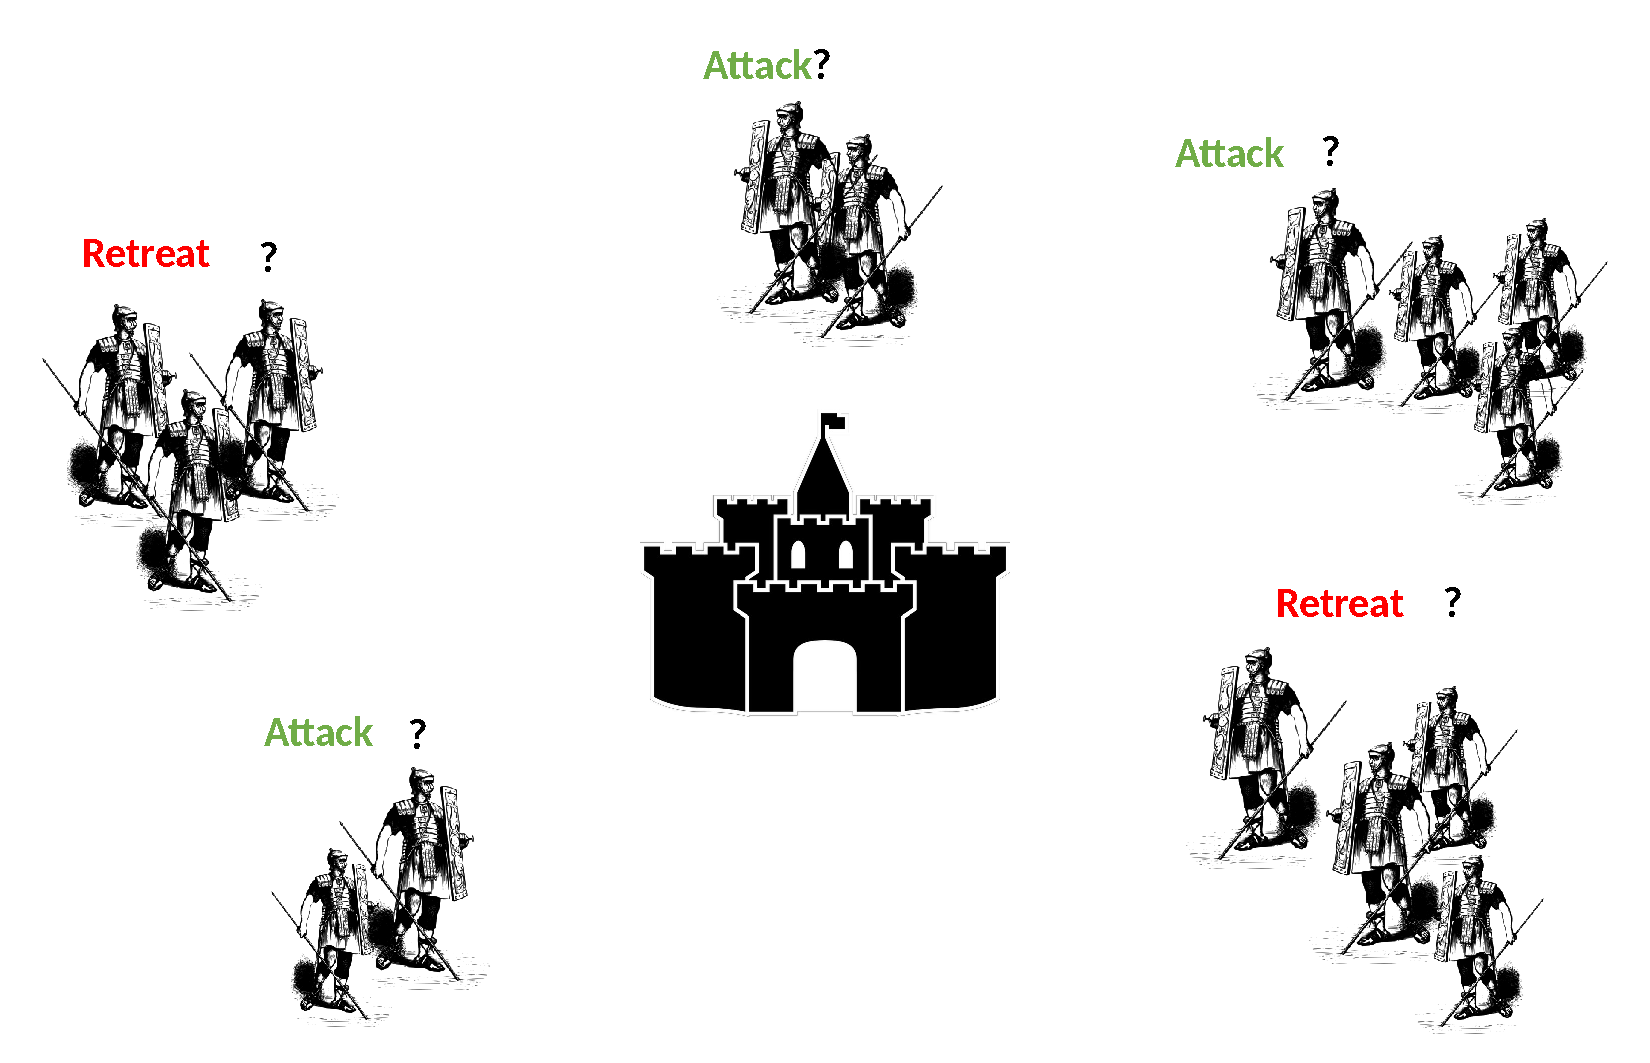
\includegraphics[width=0.85\textwidth,height=\textheight]{figuras/problema-generais-bizantinos.pdf}

\begin{itemize}
\tightlist
\item
  Atacar ou recuar? O \textbf{Consenso} é necessário para vencer.
\end{itemize}

\framebreak

\begin{itemize}
\tightlist
\item
  Em \(1982\), um experimento foi proposto por Lamport e outros em um
  artigo (\protect\hyperlink{ref-lamport1982the}{Lamport, Shostak, and
  Pease 1982}), \textbf{The Byzantine Generals Problem}.
\end{itemize}

\begin{itemize}
\item
  Como analogia a sistemas distribuídos, os generais podem ser
  considerado os \textbf{nós}, os traidores como \textbf{nós bizantinos}
  (maliciosos), e o mensageiro pode ser pensado como um canal de
  comunicação entre os generais.
\item
  O problema foi resolvido em \(1999\) por Castro e Liskov, apresentaram
  o algoritmo \emph{Practical Byzantine Fault Tolerance (PBFT)}
  (\protect\hyperlink{ref-10.5555ux2f296806.296824}{Castro and Liskov
  1999}), onde o consenso é alcançado depois de um certo número de
  mensagens serem recebidas contendo o mesmo conteúdo assinado.
\end{itemize}
\end{frame}

\begin{frame}[allowframebreaks,fragile]{Design de Sistemas Distribuídos}
\protect\hypertarget{design-de-sistemas-distribuuxeddos}{}
\begin{figure}
\centering
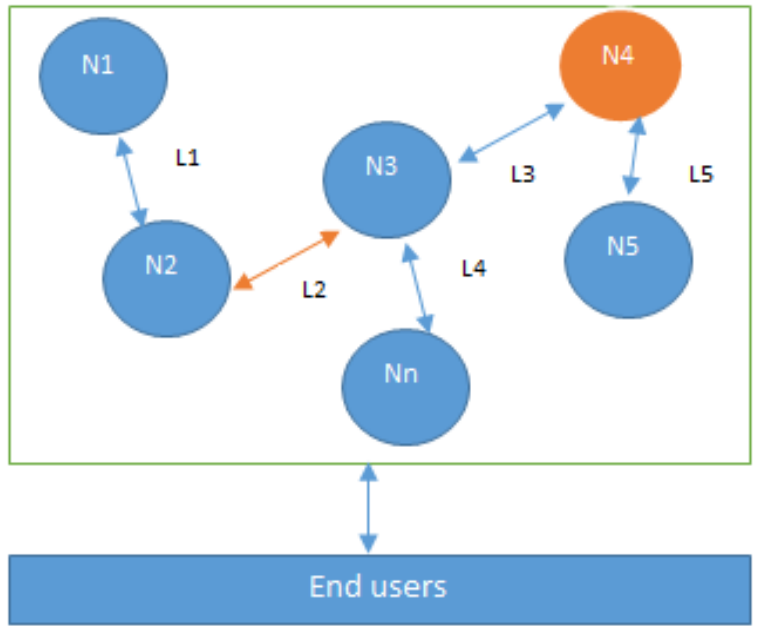
\includegraphics[width=0.7\textwidth,height=\textheight]{figuras/design-sistema-distribuido.png}
\caption{N4 é um nó Bizantino, L2 está quebrado ou é um link de rede
lento}
\end{figure}
\end{frame}

\begin{frame}[allowframebreaks,fragile]{Teorema CAP}
\protect\hypertarget{teorema-cap}{}
\begin{itemize}
\item
  Ele afirma que um Sistema Distribuído pode não ter todas as três
  propriedades desejadas simultaneamente. Sendo elas:

  \begin{itemize}
  \tightlist
  \item
    Consistency
  \item
    Availability
  \item
    Partition tolerance
  \end{itemize}
\end{itemize}

\framebreak

\begin{columns}[T]
\begin{column}{0.5\textwidth}
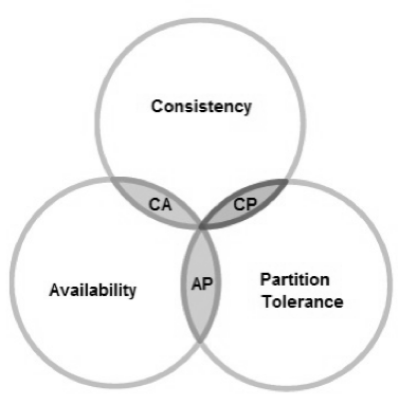
\includegraphics[width=0.75\textwidth,height=\textheight]{figuras/CAP.png}
\end{column}

\begin{column}{0.5\textwidth}
\footnotesize

\textbf{CA} - os dados estão consistentes em todos os nós, e todos os
nós estão \emph{online}.

\textbf{CP} - os dados estão consistentes em todos os nós, e mantém
\emph{partition tolerance} (prevenindo dessincronizações), torna-se
indisponível quando um nó fica inativo.

\textbf{AP} - os nós permanecem \emph{online} mesmo que não possam se
comunicar entre si. Ressincronizarão os dados assim que a partição for
resolvida, mas não há garantia de que todos os nós terão os mesmos dados
(durante ou após a partição). \normalsize
\end{column}
\end{columns}
\end{frame}

\begin{frame}{Tipos de falhas em Sistemas Distribuídos}
\protect\hypertarget{tipos-de-falhas-em-sistemas-distribuuxeddos}{}
\begin{itemize}
\tightlist
\item
  \emph{Fail-stop faults (crash faults)}

  \begin{itemize}
  \tightlist
  \item
    Onde os componentes falham ou param de operar
  \item
    Mais simples de lidar
  \end{itemize}
\item
  \emph{Byzantine faults}

  \begin{itemize}
  \tightlist
  \item
    As quais os componentes são potencialmente não confiáveis ou
    maliciosos
  \item
    Difícil de lidar
  \end{itemize}
\end{itemize}
\end{frame}

\hypertarget{conceitos-e-fundamentos-de-blockchain}{%
\section{Conceitos e Fundamentos de
Blockchain}\label{conceitos-e-fundamentos-de-blockchain}}

\begin{frame}[allowframebreaks]{Definição de Blockchain}
\protect\hypertarget{definiuxe7uxe3o-de-blockchain}{}
\begin{alertblock}{Definição de Layman}

\emph{Blockchain is an ever-growing, secure, shared recordkeeping system
in which each user of the data holds a copy of the records, which can
only be updated if all parties involved in a transaction agree to
update.}

\end{alertblock}

\begin{alertblock}{Definição Técnica}

\emph{Blockchain is a peer-to-peer distributed ledger that is
cryptographically-secure, append-only, immutable (extremely hard to
change), and updateable only via consensus or agreement among peers.}

\end{alertblock}

\framebreak

\begin{itemize}
\tightlist
\item
  \emph{Peer-to-peer}
\item
  \emph{Distributed Ledger}
\item
  \emph{Criptograficamente Seguro}
\item
  \emph{Append only (Permitido anexar novos blocos)}
\item
  \emph{Atualizável via consenso dos pares.}
\end{itemize}
\end{frame}

\begin{frame}[allowframebreaks]{Como a Tecnologia Blockchain foi
desenvolvida}
\protect\hypertarget{como-a-tecnologia-blockchain-foi-desenvolvida}{}
\begin{columns}[T]

\column{0.5\textwidth}

\textbf{1950s} -- Hash functions

\textbf{1970s} -- Merkle trees - hashes in a tree structure

\textbf{1970s} continued -- Research in distributed systems, consensus,
state machine replication

\textbf{1980s} -- Hash chains for secure logins

\textbf{1990s} -- \emph{e-Cash for e-payments}

\column{0.5\textwidth}

\textbf{1991} -- Secure timestamping of digital documents.

\textbf{1992} -- Hashcash idea to combat junk emails

\textbf{1994} -- S/KEY application for Unix login.

\textbf{1997/2002} -- \emph{Hashcash}

\textbf{2008/2009} -- Bitcoin (the first blockchain)

\end{columns}

\framebreak

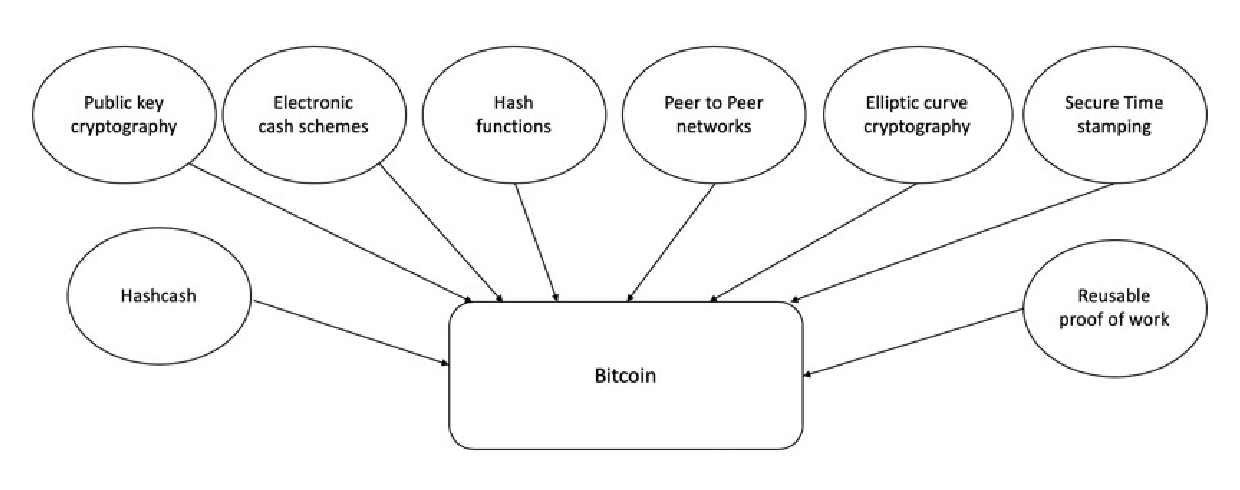
\includegraphics{figuras/ecossitema-bitcoin.pdf}
\end{frame}

\begin{frame}{Interesse no termo ``blockchain''}
\protect\hypertarget{interesse-no-termo-blockchain}{}
\begin{itemize}
\tightlist
\item
  Interesse ao longo do tempo
  (\href{https://trends.google.com/trends/explore?date=2008-01-01\%202023-04-18\&q=blockchain}{Fonte:
  Google Trends}):
\end{itemize}

\begin{figure}
\centering
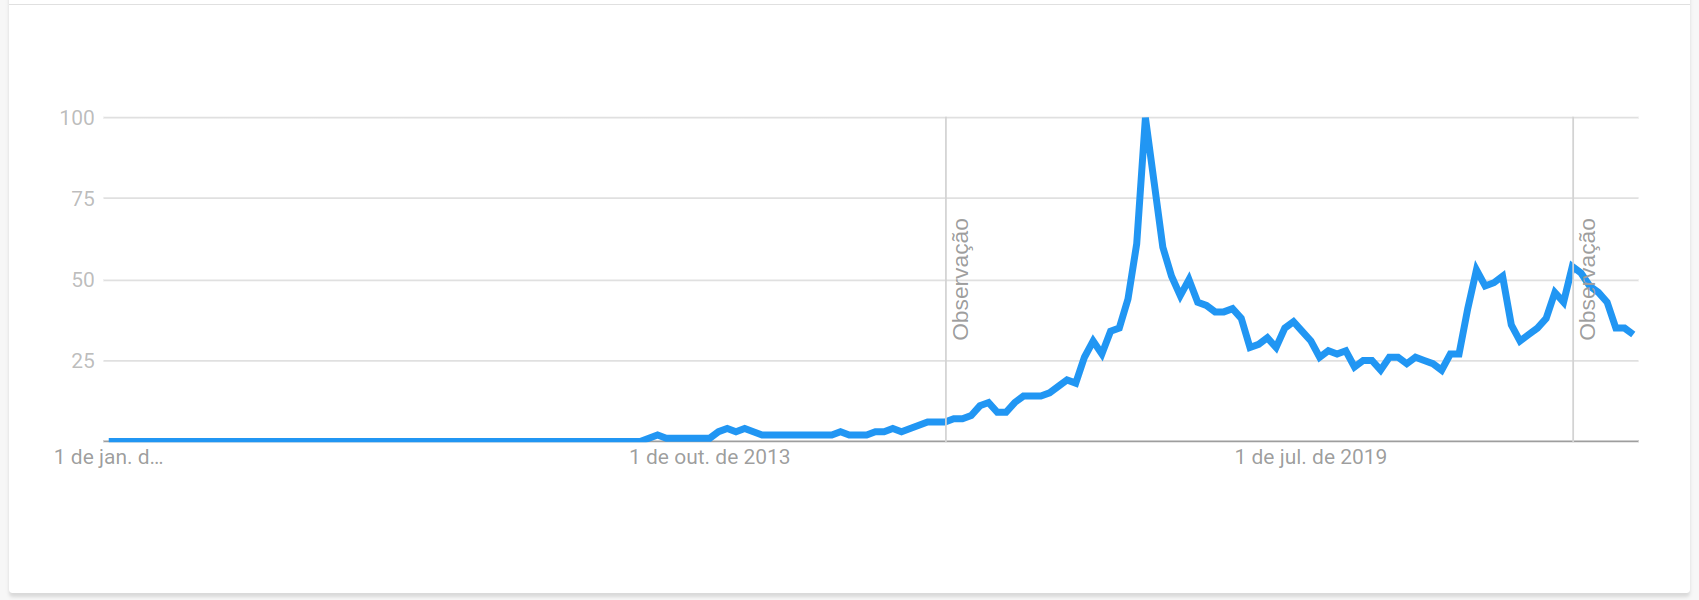
\includegraphics{figuras/interesse-termo-blockchain-2008-08-2022.png}
\caption{Pesquisas sobre o termo ``blockchain''}
\end{figure}
\end{frame}

\begin{frame}{Visão Arquitetural do Blockchain}
\protect\hypertarget{visuxe3o-arquitetural-do-blockchain}{}
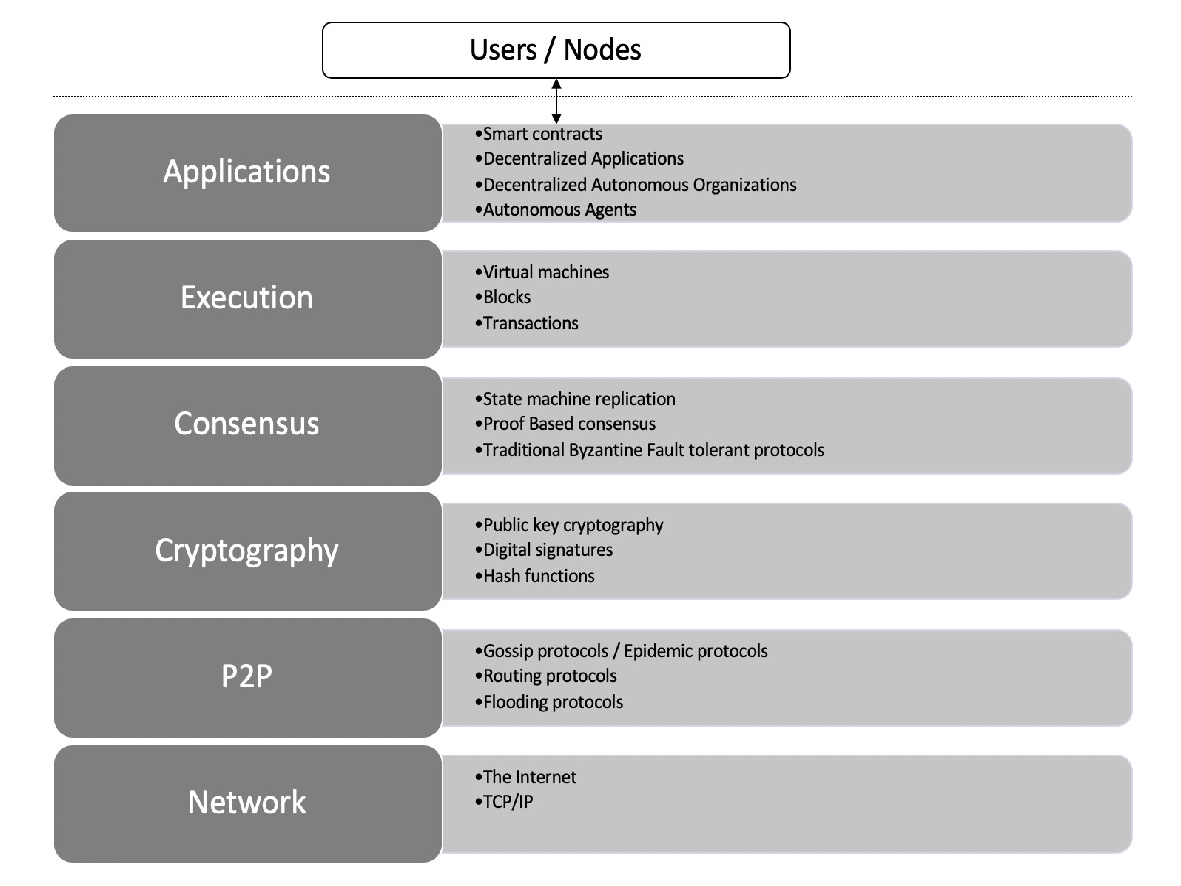
\includegraphics{figuras/visao-arquitetural-blockchain.pdf}
\end{frame}

\begin{frame}[allowframebreaks]{Estrutura Genérica de um Blockchain}
\protect\hypertarget{estrutura-genuxe9rica-de-um-blockchain}{}
\begin{figure}
\centering
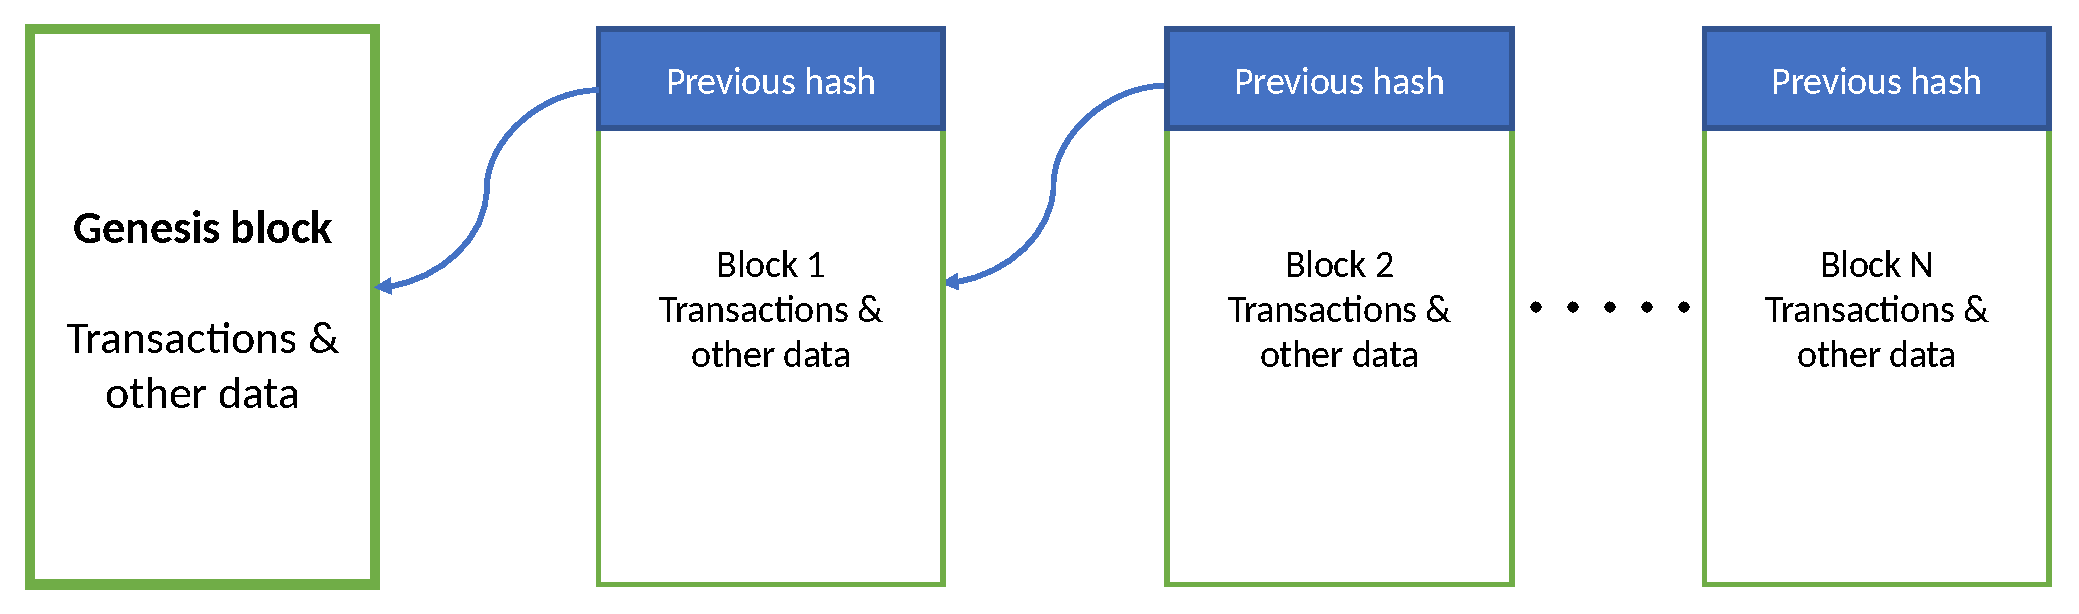
\includegraphics[width=1\textwidth,height=\textheight]{figuras/estrutura-generica-blockchain.pdf}
\caption{Estrutura Genérica de um Blockchain}
\end{figure}
\end{frame}

\begin{frame}[allowframebreaks]{Elementos Genéricos de um Blockchain}
\protect\hypertarget{elementos-genuxe9ricos-de-um-blockchain}{}
\begin{itemize}
\tightlist
\item
  Endereços
\item
  Contas
\item
  Transações
\item
  Blocos
\item
  Redes \emph{Peer-to-peer}
\item
  Scripting ou Linguagens de Programação
\item
  Virtual machines
\item
  Máquinas de Estado
\item
  Nós (nodes)
\item
  Contratos Inteligentes \emph{(Smart contracts)}
\end{itemize}
\end{frame}

\begin{frame}[allowframebreaks]{Como um Blockchain funciona}
\protect\hypertarget{como-um-blockchain-funciona}{}
\begin{figure}
\centering
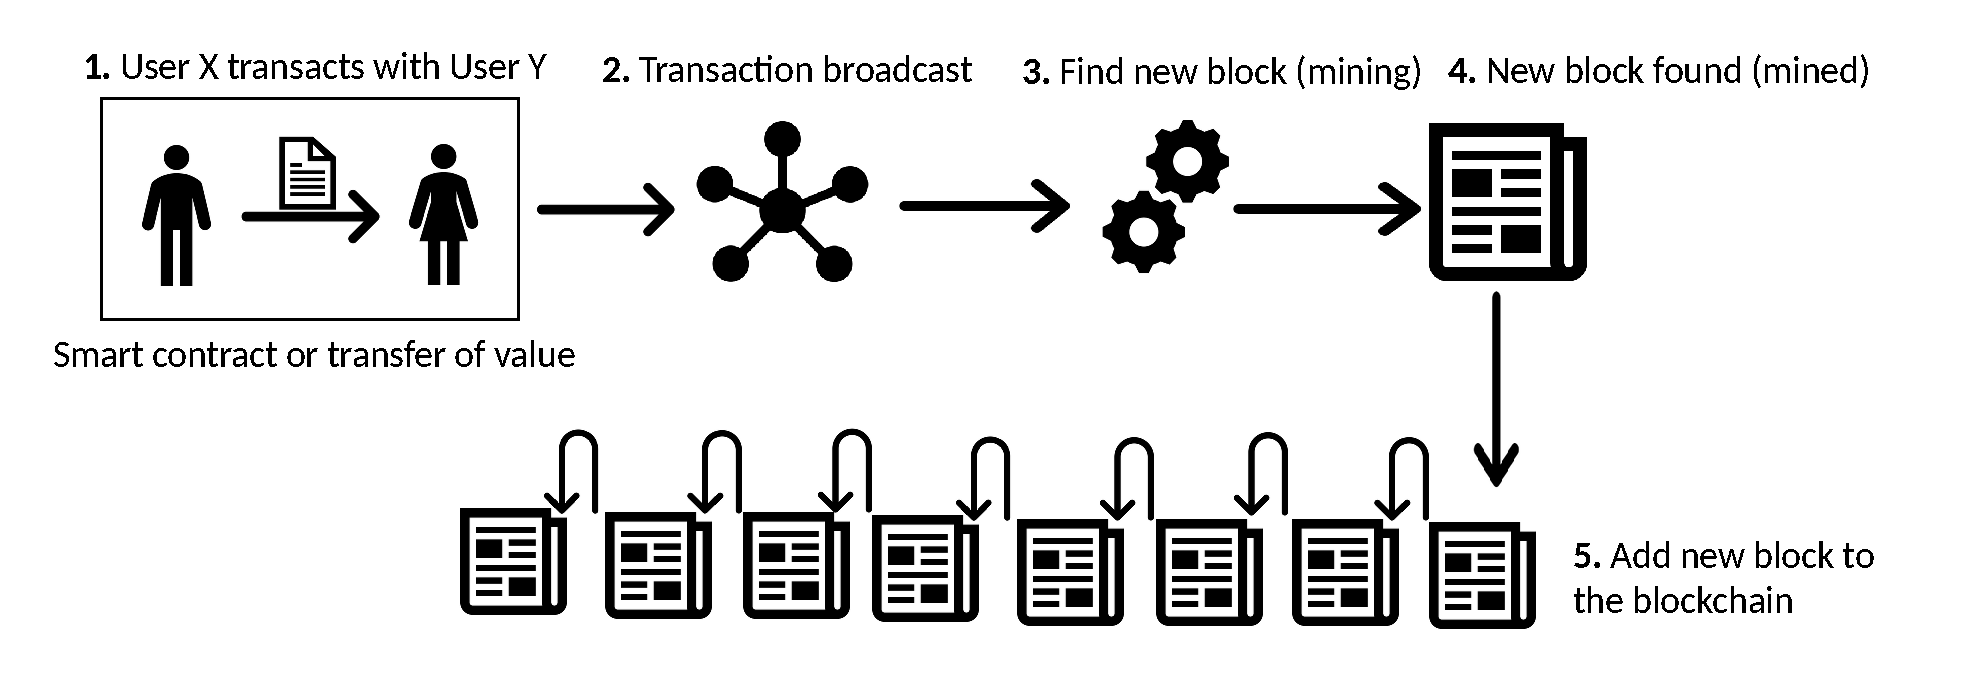
\includegraphics{figuras/funcionamento-blockchain.pdf}
\caption{Funcionamento de um Blockchain}
\end{figure}
\end{frame}

\begin{frame}[allowframebreaks]{Estrutura Genérica de um bloco}
\protect\hypertarget{estrutura-genuxe9rica-de-um-bloco}{}
\begin{figure}
\centering
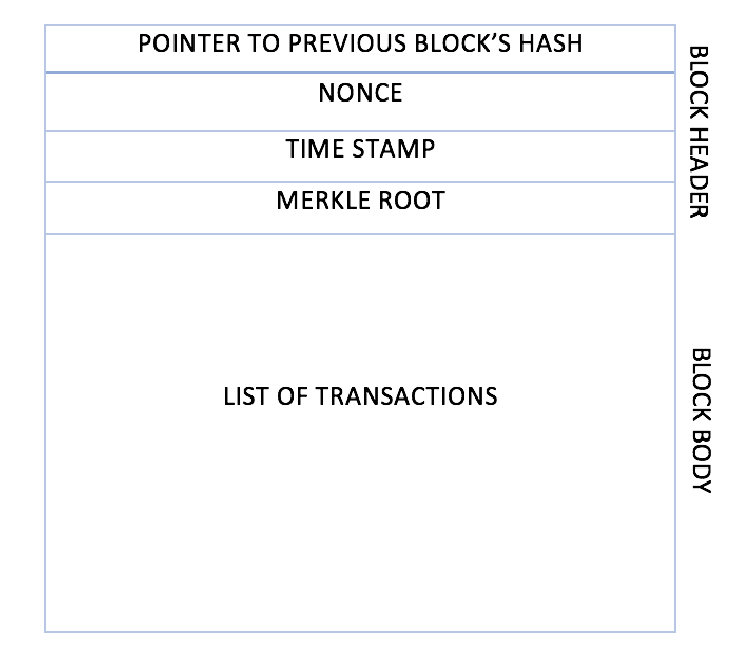
\includegraphics[width=0.6\textwidth,height=\textheight]{figuras/estrutura-generica-de-bloco.pdf}
\caption{Estrutura de um Bloco}
\end{figure}
\end{frame}

\begin{frame}{Benefícios e Limitações de um Blockchain}
\protect\hypertarget{benefuxedcios-e-limitauxe7uxf5es-de-um-blockchain}{}
\begin{columns}[T]

\column{0.5\textwidth}

\textbf{Benefícios}

Descentralização

Transparência

Confiança

Imutabilidade

Alta disponibilidade

Altamente Seguro

Simplificação de paradigmas atuais

Transações rápidas

Cost saving

\column{0.5\textwidth}

\textbf{Limitações}

Escalabilidade

Adaptabilidade

Regulação

Tecnologia Relativamente Imatura

Privacidade

\end{columns}
\end{frame}

\begin{frame}[allowframebreaks]{Características Principais}
\protect\hypertarget{caracteruxedsticas-principais}{}
\begin{itemize}
\item
  Consenso Distribuído
\item
  Verificação de Transações
\item
  Plataforma para \emph{smart contracts}
\item
  Transferência de valores entre pares
\item
  Generação de criptomoedas
\item
  Provedor de Segurança
\item
  Imutabilidade
\item
  Unicidade ou singularidade (Uniqueness)
\end{itemize}
\end{frame}

\begin{frame}{Atividade}
\protect\hypertarget{atividade}{}
\begin{alertblock}{Leitura}

\emph{Bitcoin paper}: \url{https://bitcoin.org/bitcoin.pdf}

\end{alertblock}
\end{frame}

\begin{frame}{Leitura Recomendada}
\protect\hypertarget{leitura-recomendada}{}
\normalsize

\begin{alertblock}{Leitura Recomendada}

\textbf{Capítulo 1: Blockchain 101}

\textbf{Livro}:
\href{https://search.ebscohost.com/login.aspx?direct=true\&db=e000xww\&AN=1789486\&lang=pt-br\&site=eds-live\&scope=site\&ebv=EB\&ppid=pp_8}{IMRAN
BASHIR. Mastering Blockchain\,: Distributed Ledger Technology,
Decentralization, and Smart Contracts Explained, 2nd Edition.}

\end{alertblock}
\end{frame}

\hypertarget{bitcoin}{%
\section{Bitcoin}\label{bitcoin}}

\begin{frame}[allowframebreaks]{Bitcoin na perspectiva de usuário~}
\protect\hypertarget{bitcoin-na-perspectiva-de-usuuxe1rio}{}
\begin{itemize}
\tightlist
\item
  Passos de como enviar e receber pagamentos:

  \begin{itemize}
  \tightlist
  \item
    A transação começa com um remetente assinando a transação com sua
    chave privada.~
  \item
    A transação é serializada para que possa ser transmitida pela rede.
  \item
    A transação é transmitida para a rede.
  \item
    Mineradores que escutam transações pegam a transação.
  \item
    A transação é verificada quanto à sua legitimidade pelos
    mineradores.
  \item
    A transação é adicionada ao bloco candidato/proposto para mineração.
  \item
    Uma vez minerado, o resultado é transmitido para todos os nós da
    rede \emph{Bitcoin}.
  \item
    Normalmente, neste momento, os usuários aguardam até seis
    confirmações para serem recebidas antes que uma transação seja
    considerada final; no entanto, uma transação pode ser considerada
    final na etapa anterior.
  \item
    As confirmações servem como um mecanismo adicional para garantir que
    haja probabilidade muito baixa de uma transação ser revertida, mas,
    caso contrário, uma vez que um bloco minerado seja finalizado e
    anunciado, as transações dentro desse bloco serão finais nesse
    ponto.
  \end{itemize}
\end{itemize}
\end{frame}

\begin{frame}[allowframebreaks]{Chaves Criptográficas~}
\protect\hypertarget{chaves-criptogruxe1ficas}{}
\begin{columns}[T]

\column{0.5\textwidth}

\begin{itemize}
\tightlist
\item
  Private keys in Bitcoin~

  \begin{itemize}
  \tightlist
  \item
    Private keys are used to digitally sign the transactions, proving
    ownership of the bitcoins.
  \end{itemize}
\item
  Public keys in Bitcoin~

  \begin{itemize}
  \tightlist
  \item
    Public keys are used by nodes to verify that the transaction has
    indeed been signed with the corresponding private key.
  \end{itemize}
\item
  Addresses in Bitcoin~

  \begin{itemize}
  \tightlist
  \item
    A Bitcoin address is created by taking the corresponding public key
    of a private key and hashing it twice, first with the SHA256
    algorithm and then with RIPEMD160.
  \end{itemize}
\item
  Bitcoin addresses are encoded using \textbf{Base58Check} encoding
\end{itemize}

\column{0.5\textwidth}


\includegraphics{figuras/qrcode-bitcoin-address.pdf}

\end{columns}
\end{frame}

\begin{frame}[allowframebreaks]{Geração de Endereços no Bitcoin}
\protect\hypertarget{gerauxe7uxe3o-de-endereuxe7os-no-bitcoin}{}
\begin{itemize}
\tightlist
\item
  Para gerar um endereço no \textbf{Bitcoin}, é usado um processo de
  \(11\) etapas:
\end{itemize}

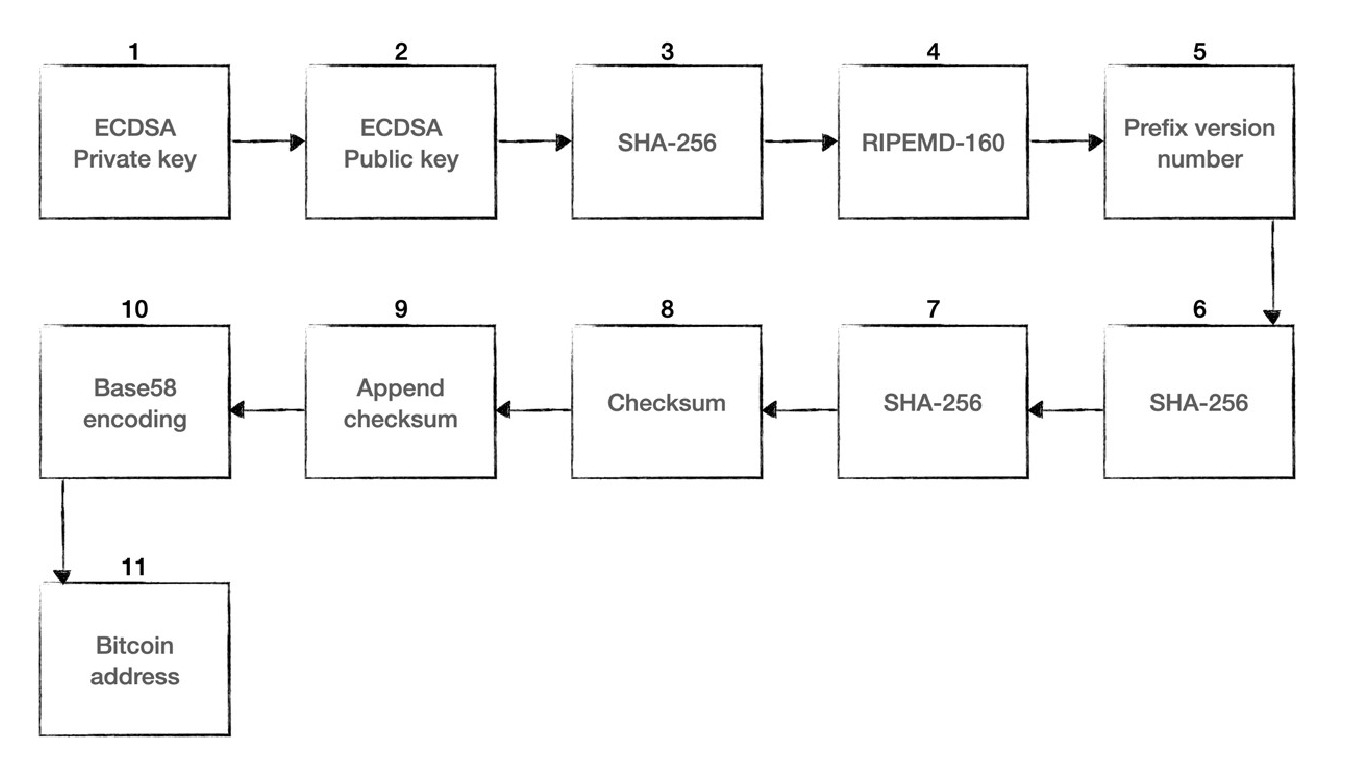
\includegraphics[width=0.9\textwidth,height=\textheight]{figuras/bitcoin-address-generation.pdf}
\end{frame}

\begin{frame}[allowframebreaks]{Transações}
\protect\hypertarget{transauxe7uxf5es}{}
\begin{itemize}
\tightlist
\item
  A user/sender sends a transaction using wallet software or some other
  interface.~
\item
  The transaction is signed using the sender's private key.~
\item
  The transaction is broadcasted to the Bitcoin network using a flooding
  algorithm.~
\item
  Mining nodes (miners) who are listening for the transactions verify
  and include this transaction in the next lock to be mined.
\item
  Next, the mining starts.~
\item
  Finally, the confirmations start to appear in the receiver's wallet.~
\end{itemize}
\end{frame}

\begin{frame}[allowframebreaks]{Estrutura de dados de uma Transação~}
\protect\hypertarget{estrutura-de-dados-de-uma-transauxe7uxe3o}{}
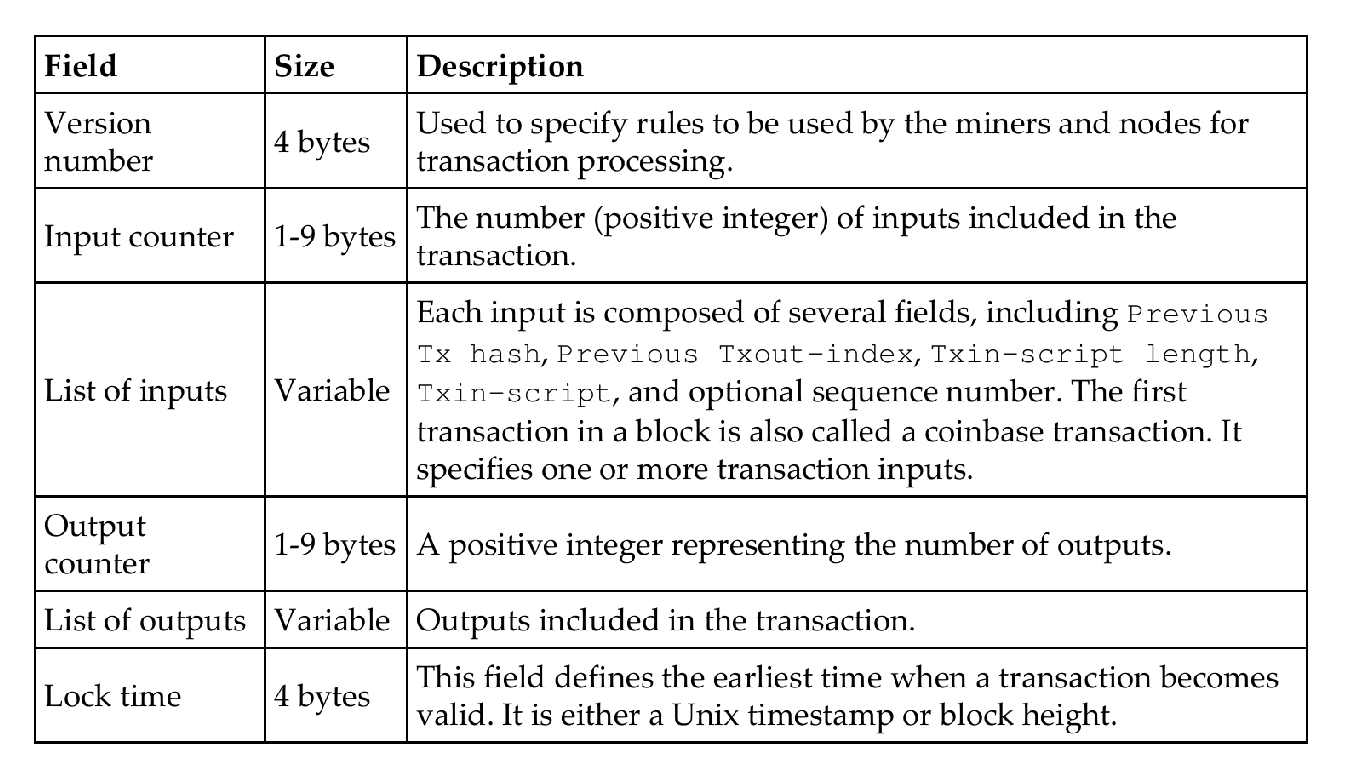
\includegraphics[width=1\textwidth,height=\textheight]{figuras/transaction-data-sctruture.pdf}
\end{frame}

\begin{frame}[allowframebreaks]{Estrutura de dados de uma Transação~--
entradas e saídas}
\protect\hypertarget{estrutura-de-dados-de-uma-transauxe7uxe3o-entradas-e-sauxeddas}{}
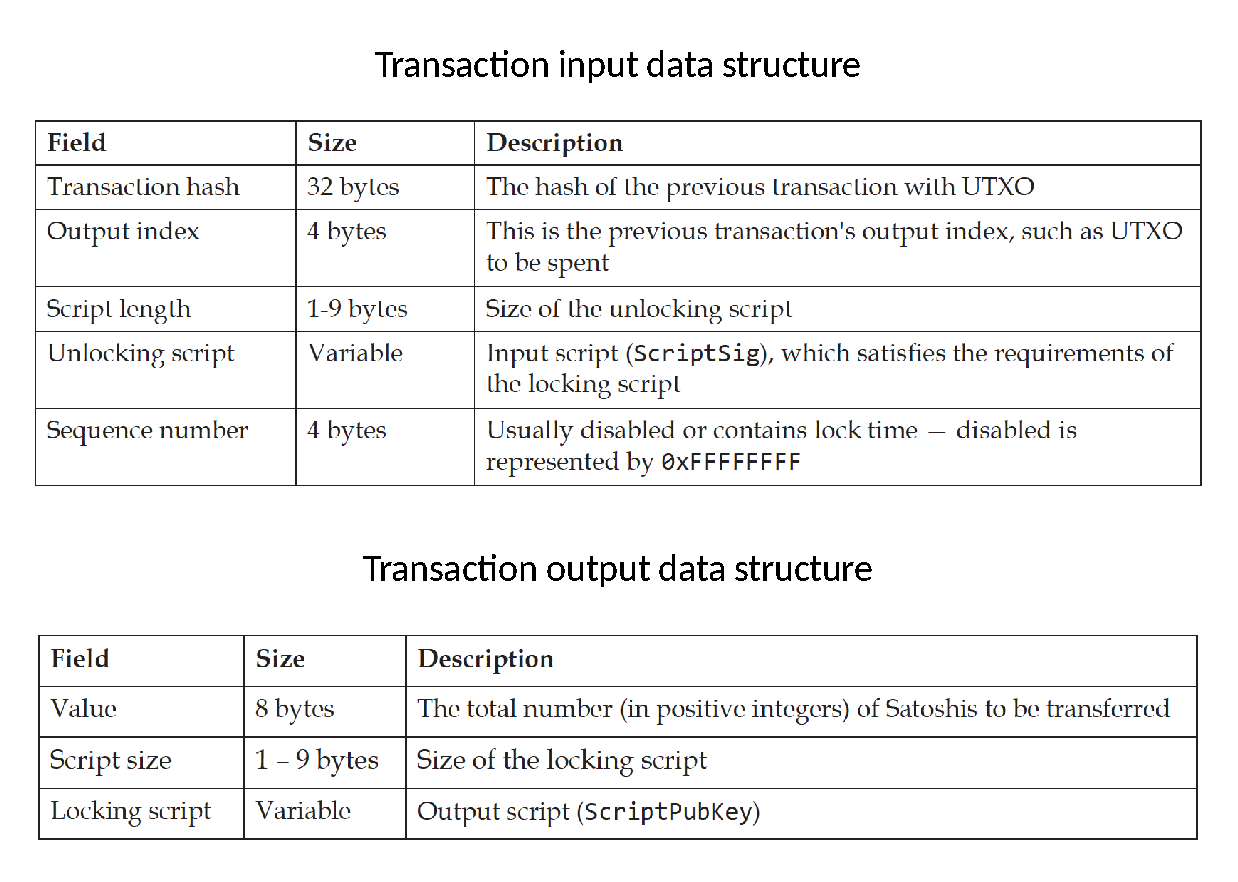
\includegraphics[width=0.9\textwidth,height=\textheight]{figuras/transaction-data-sctruture-inouts.pdf}
\end{frame}

\begin{frame}[allowframebreaks]{Script}
\protect\hypertarget{script}{}
\begin{itemize}
\tightlist
\item
  Simple stack-based language used to describe how bitcoins can be spent
  and transferred
\item
  Evaluated from left to right using a Last in, First Out (LIFO) stack
\item
  Composed of two components: elements and operations.
\item
  Scripts use various operations (opcodes) to define their operations.
\end{itemize}
\end{frame}

\begin{frame}[allowframebreaks]{Opcodes}
\protect\hypertarget{opcodes}{}
\begin{itemize}
\tightlist
\item
  Here are some examples of a few useful opcodes used in the Script
  language on the Bitcoin blockchain.
\end{itemize}

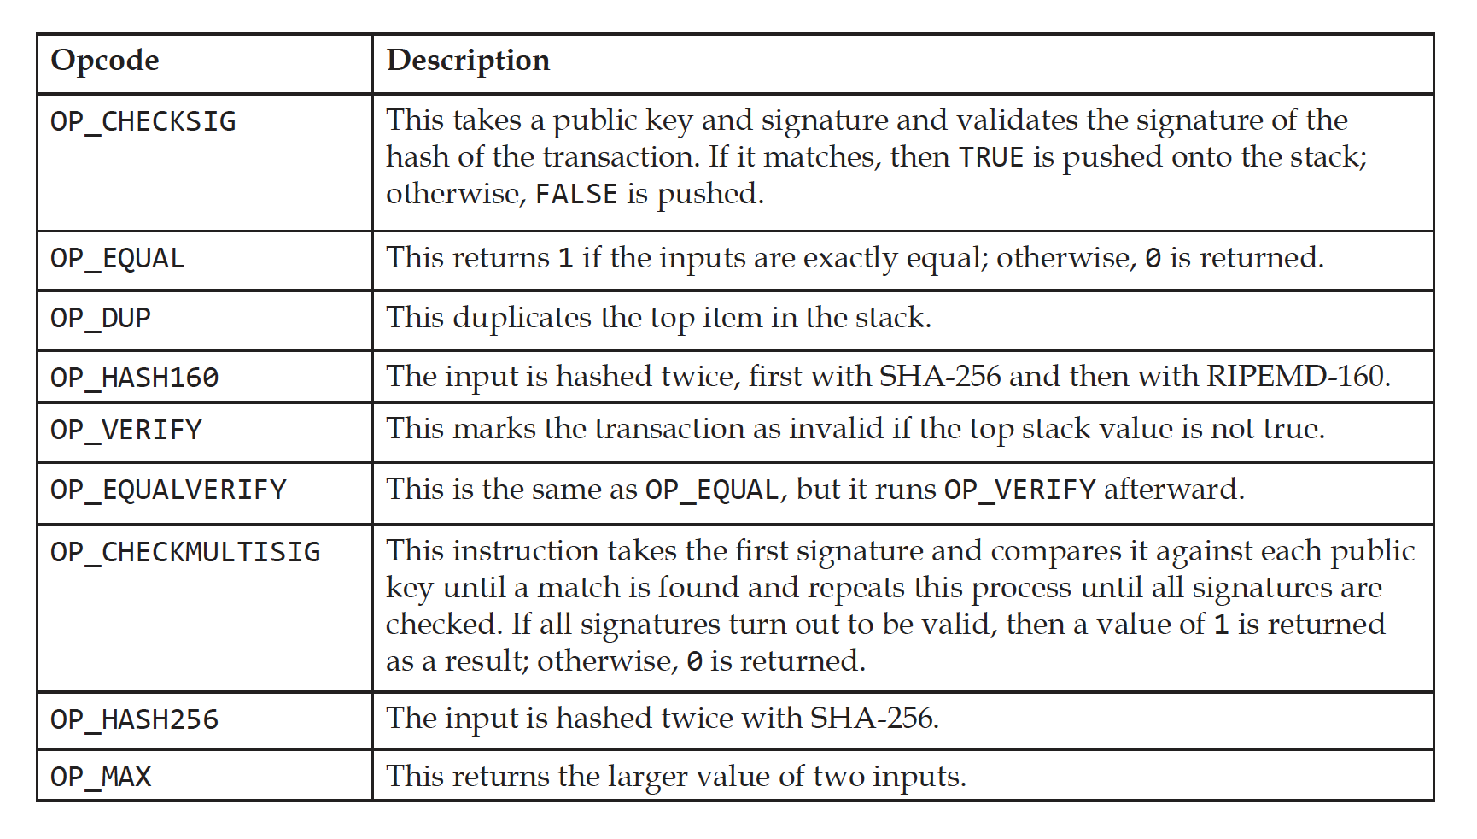
\includegraphics{figuras/opcodes.pdf}
\end{frame}

\begin{frame}[allowframebreaks]{P2PKH script execution~}
\protect\hypertarget{p2pkh-script-execution}{}
\begin{itemize}
\tightlist
\item
  P2PKH is the most commonly used transaction type and is used to send
  transactions to Bitcoin addresses.
\end{itemize}

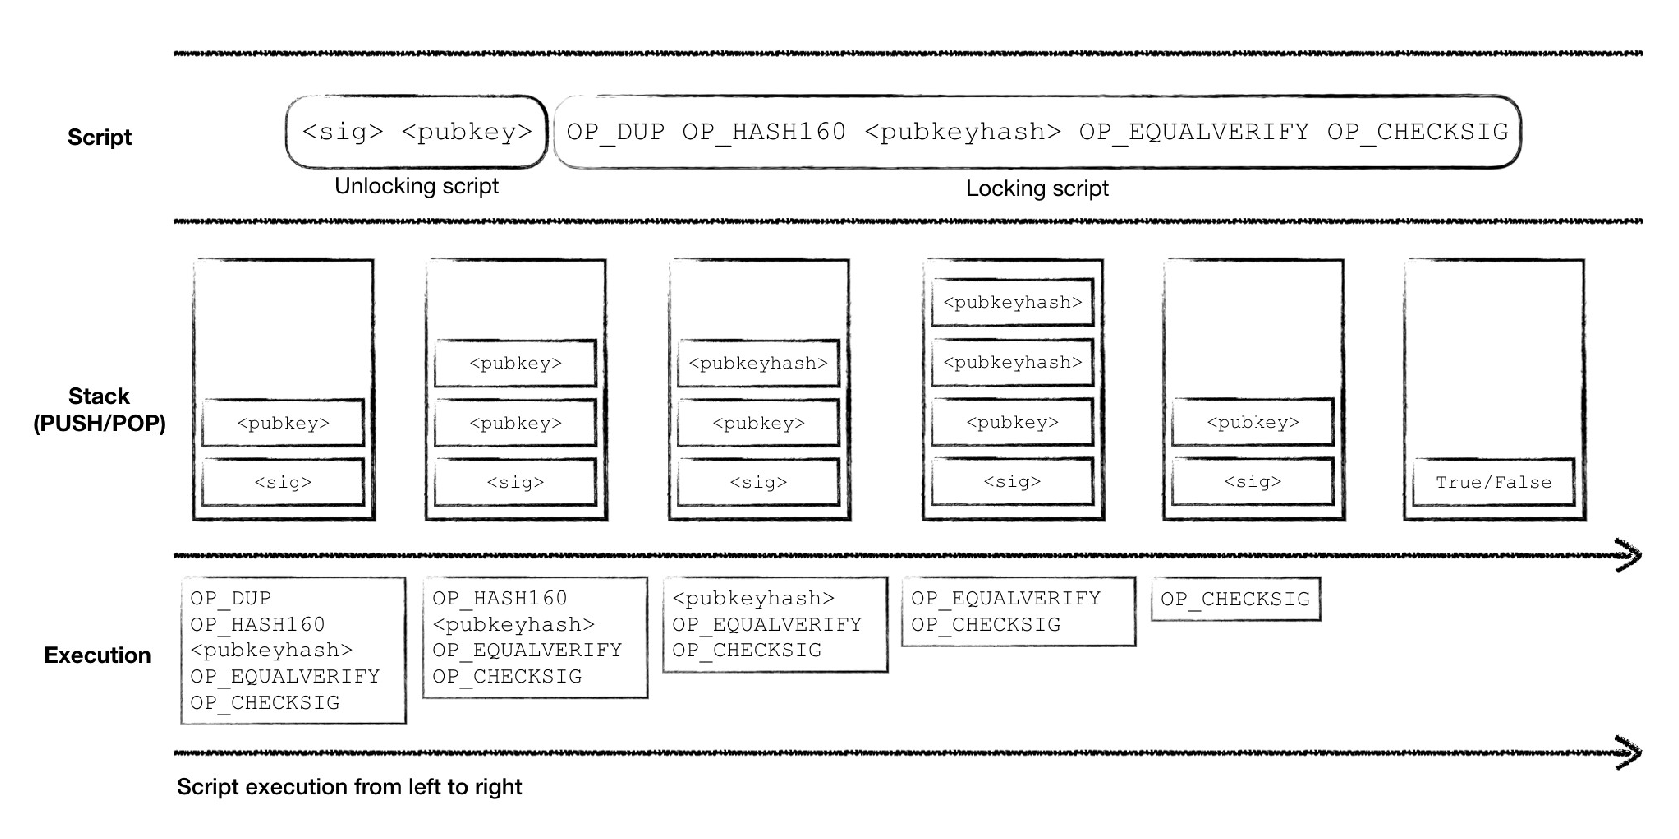
\includegraphics{figuras/p2pkh-execution.pdf}
\end{frame}

\begin{frame}[allowframebreaks]{Validação de Transações~}
\protect\hypertarget{validauxe7uxe3o-de-transauxe7uxf5es}{}
During validation, the following are checked:

\begin{itemize}
\item
  That transaction inputs are previously unspent. This validation step
  prevents double-spending by verifying that the transaction inputs have
  not already been spent by someone else.
\item
  That the sum of the transaction outputs is not more than the total sum
  of the transaction inputs. However, both input and output sums can be
  the same, or the sum of the input (total value) could be more than the
  total value of the outputs. This check ensures that no new bitcoins
  are created out of thin air.~
\item
  That that the digital signatures are valid, which ensures that the
  script is valid.
\end{itemize}
\end{frame}

\begin{frame}[allowframebreaks]{Blocos}
\protect\hypertarget{blocos}{}
\begin{itemize}
\tightlist
\item
  A estrutura de um Bloco Bitcoin é mostrado na tabela:
\end{itemize}

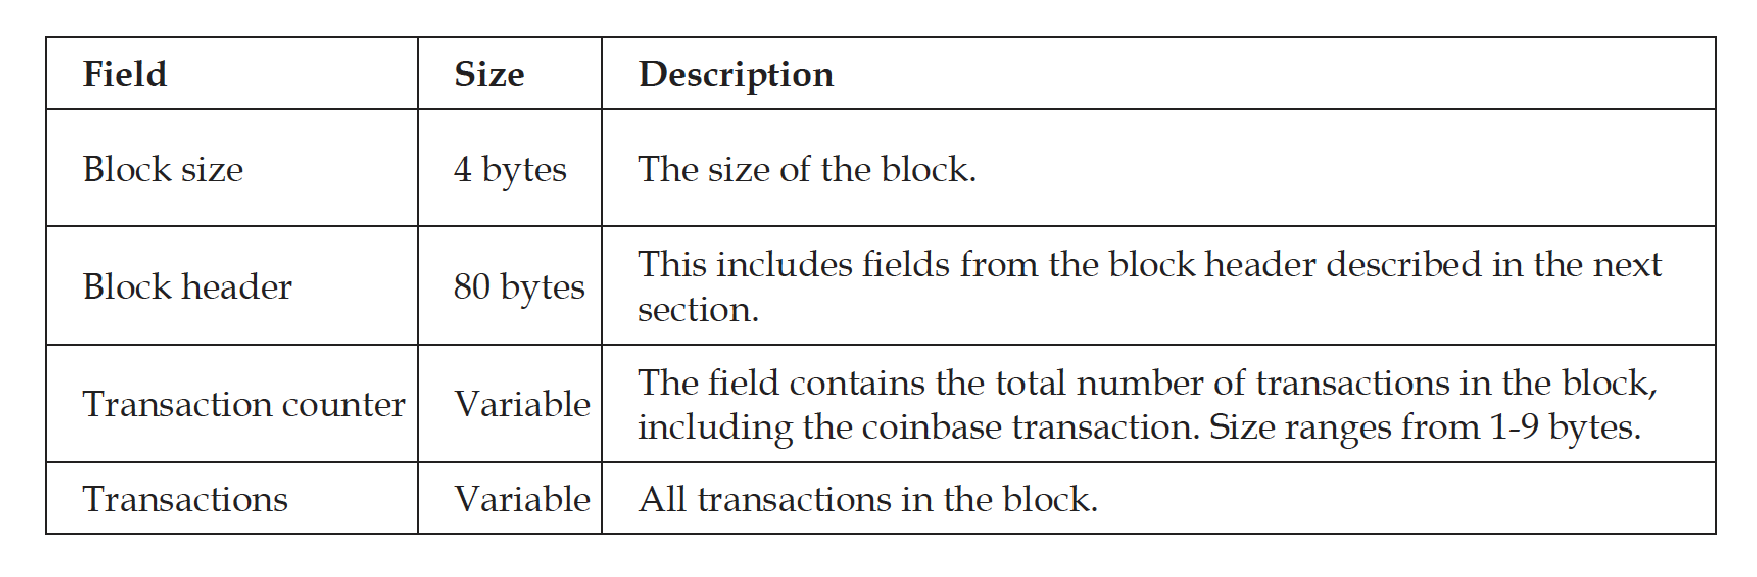
\includegraphics[width=1\textwidth,height=\textheight]{figuras/bitcoin-bloco.pdf}

\framebreak

\begin{itemize}
\tightlist
\item
  A estrutura do cabeçalho de um bloco:
\end{itemize}

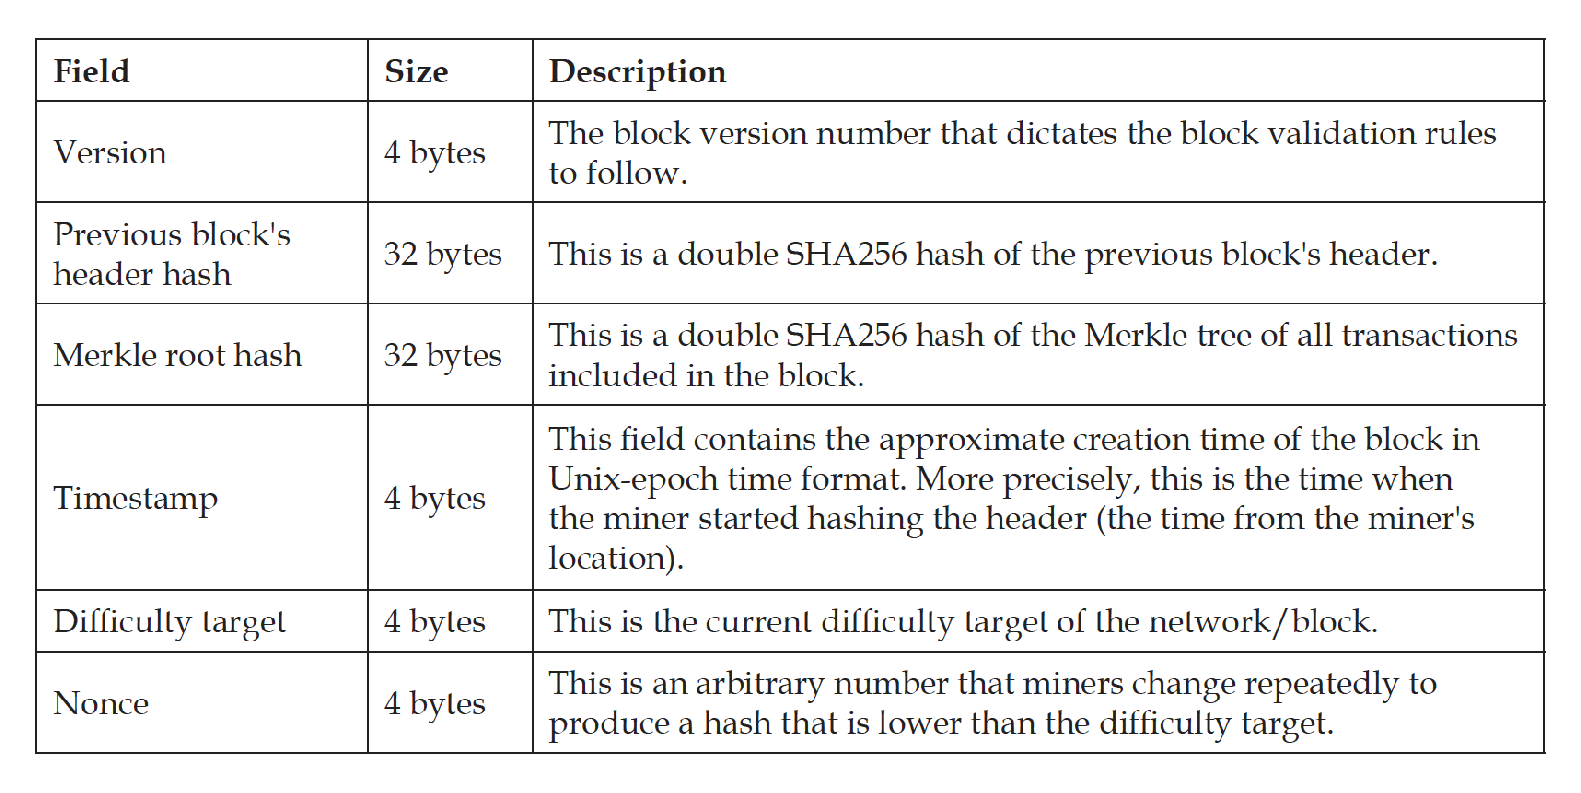
\includegraphics[width=1\textwidth,height=\textheight]{figuras/bitcoin-bloco-header.pdf}
\end{frame}

\begin{frame}[allowframebreaks]{Uma Visualização da Blockchain do
Bitcoin}
\protect\hypertarget{uma-visualizauxe7uxe3o-da-blockchain-do-bitcoin}{}
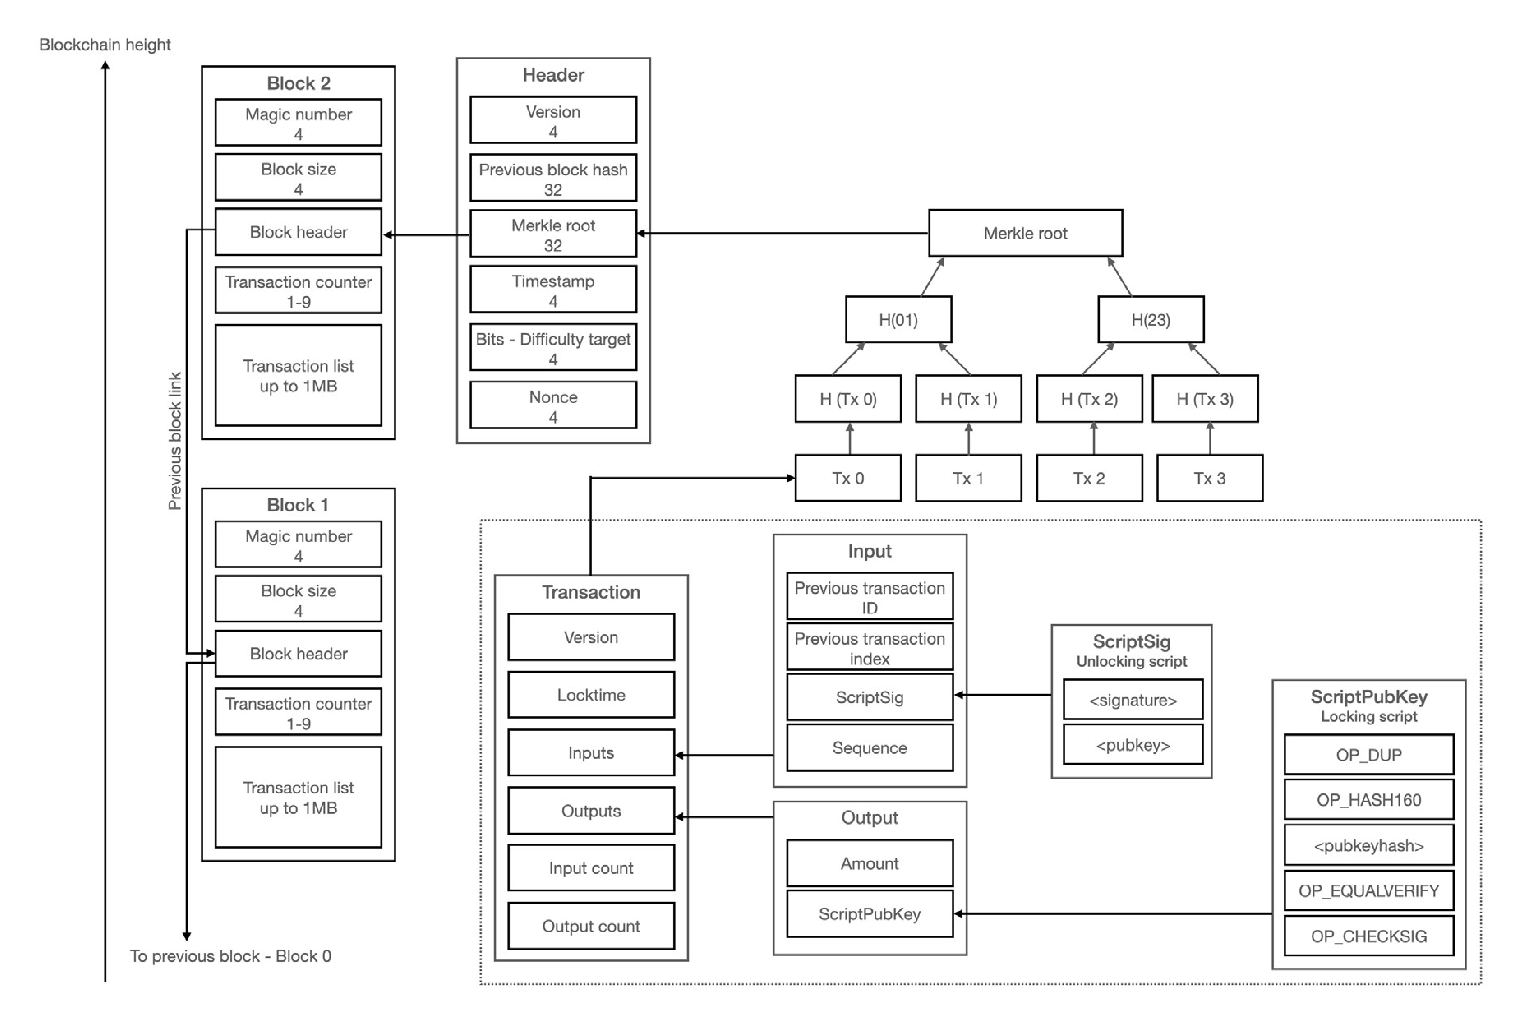
\includegraphics[width=1\textwidth,height=\textheight]{figuras/bitcoin-blockchain.pdf}
\end{frame}

\begin{frame}[allowframebreaks,fragile]{Bloco Genesis}
\protect\hypertarget{bloco-genesis}{}
\begin{alertblock}{Bloco Genesis}

O Bloco Genesis ou bloco \(\#0\) foi \emph{hardcoded} (codificado) por
suas características especiais: ele é o único que não aponta para nenhum
bloco anterior. No seu \emph{hash} foi encriptado o bloco junto com a
mensagem \emph{``The Times 03/Jan/2009 Chancellor on brink of second
bailout for banks''}, manchete do jornal naquele dia. Além de servir
como prova datada, a manchete escolhida representa justamente uma
crítica ao sistema bancário.

\end{alertblock}

\framebreak

\begin{columns}[T]

\column{0.5\textwidth}


\includegraphics{figuras/thetimes03-01-2009-1.jpg}

\column{0.5\textwidth}

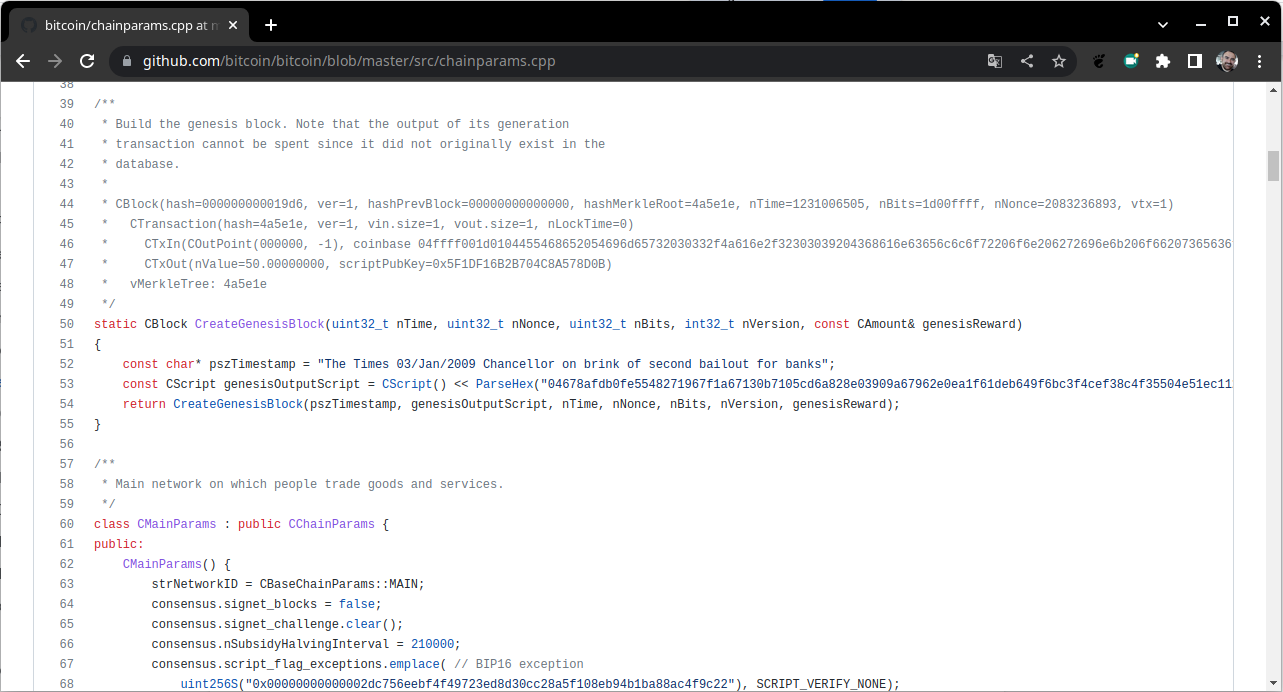
\includegraphics{figuras/genesis-block-github.png}

\scriptsize

\textbf{Fonte:}
\url{https://github.com/bitcoin/bitcoin/blob/master/src/chainparams.cpp}

\end{columns}

\framebreak

\tiny

\begin{Shaded}
\begin{Highlighting}[]
\CommentTok{/**}
\CommentTok{ * Build the genesis block. Note that the output of its generation}
\CommentTok{ * transaction cannot be spent since it did not originally exist in the}
\CommentTok{ * database.}
\CommentTok{ *}
\CommentTok{ * CBlock(hash=000000000019d6, ver=1, hashPrevBlock=00000000000000, hashMerkleRoot=4a5e1e, nTime=1231006505, nBits=1d00ffff, nNonce=2083236893, vtx=1)}
\CommentTok{ *   CTransaction(hash=4a5e1e, ver=1, vin.size=1, vout.size=1, nLockTime=0)}
\CommentTok{ *     CTxIn(COutPoint(000000, {-}1), coinbase 04ffff001d0104455468652054696d65732030332f4a616e2f32303039204368616e63656c6c6f72206f6e206272696e6b206f66207365636f6e64206261696c6f757420666f722062616e6b73)}
\CommentTok{ *     CTxOut(nValue=50.00000000, scriptPubKey=0x5F1DF16B2B704C8A578D0B)}
\CommentTok{ *   vMerkleTree: 4a5e1e}
\CommentTok{ */}
\AttributeTok{static}\NormalTok{ CBlock CreateGenesisBlock}\OperatorTok{(}\DataTypeTok{uint32\_t}\NormalTok{ nTime}\OperatorTok{,} \DataTypeTok{uint32\_t}\NormalTok{ nNonce}\OperatorTok{,} \DataTypeTok{uint32\_t}\NormalTok{ nBits}\OperatorTok{,} \DataTypeTok{int32\_t}\NormalTok{ nVersion}\OperatorTok{,} 
\AttributeTok{const}\NormalTok{ CAmount}\OperatorTok{\&}\NormalTok{ genesisReward}\OperatorTok{)}
\OperatorTok{\{}
  \AttributeTok{const} \DataTypeTok{char}\OperatorTok{*}\NormalTok{ pszTimestamp }\OperatorTok{=} \StringTok{"The Times 03/Jan/2009 Chancellor on brink of second bailout for banks"}\OperatorTok{;}
  \AttributeTok{const}\NormalTok{ CScript genesisOutputScript }\OperatorTok{=}\NormalTok{ CScript}\OperatorTok{()} \OperatorTok{\textless{}\textless{}}\NormalTok{ ParseHex}\OperatorTok{(}\StringTok{"04678afdb0fe5548271967f1a67130b7105cd6a828e03909a67962e0ea1f61deb649f6bc3f4cef38c4f35504e51ec112de5c384df7ba0b8d578a4c702b6bf11d5f"}\OperatorTok{)} \OperatorTok{\textless{}\textless{}}\NormalTok{ OP\_CHECKSIG}\OperatorTok{;}
  \ControlFlowTok{return}\NormalTok{ CreateGenesisBlock}\OperatorTok{(}\NormalTok{pszTimestamp}\OperatorTok{,}\NormalTok{ genesisOutputScript}\OperatorTok{,}\NormalTok{ nTime}\OperatorTok{,}\NormalTok{ nNonce}\OperatorTok{,}\NormalTok{ nBits}\OperatorTok{,}\NormalTok{ nVersion}\OperatorTok{,}\NormalTok{ genesisReward}\OperatorTok{);}
\OperatorTok{\}}
\end{Highlighting}
\end{Shaded}

\normalsize

\framebreak
\end{frame}

\begin{frame}[fragile,allowframebreaks]{A carteira de Satoshi}
\protect\hypertarget{a-carteira-de-satoshi}{}
\begin{itemize}
\tightlist
\item
  Carteira:
  \href{https://blockchair.com/bitcoin/address/1A1zP1eP5QGefi2DMPTfTL5SLmv7DivfNa}{\texttt{1A1zP1eP5QGefi2DMPTfTL5SLmv7DivfNa}}
\end{itemize}

\begin{figure}
\centering
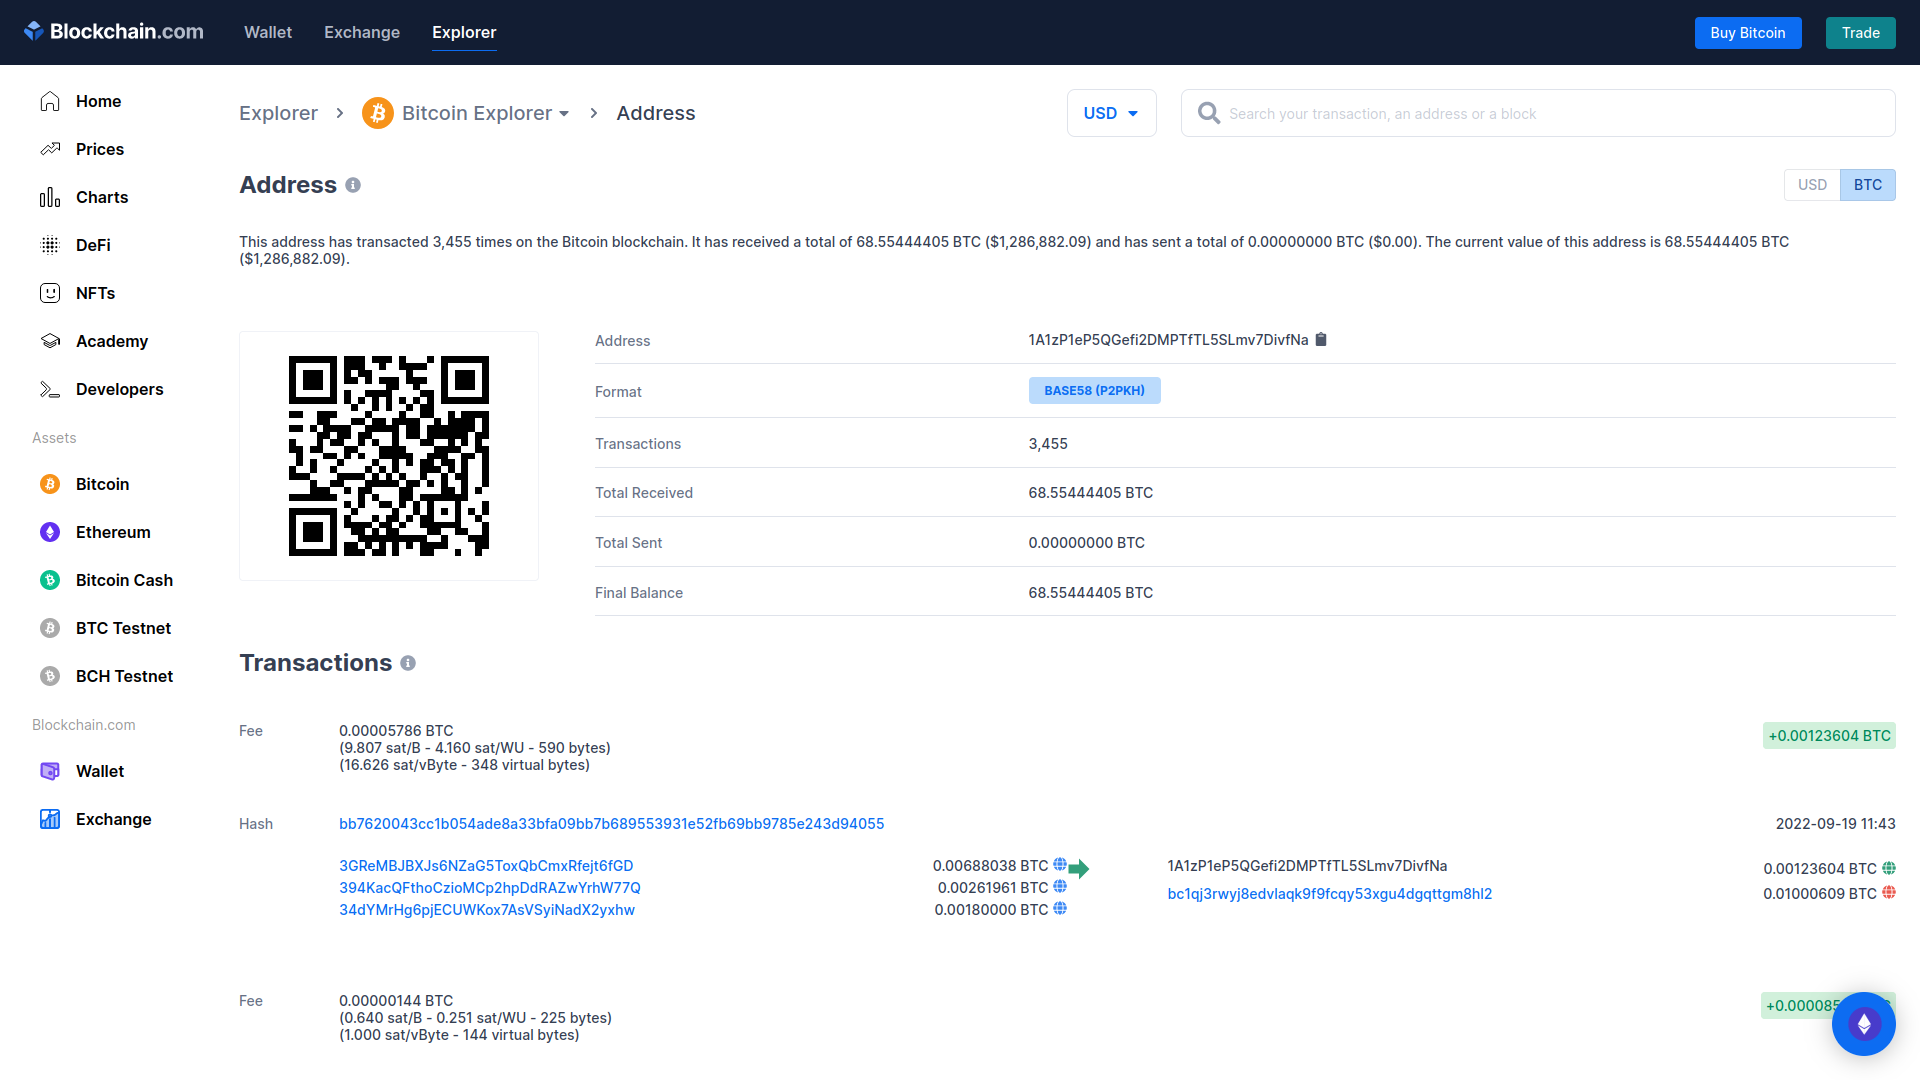
\includegraphics[width=0.9\textwidth,height=\textheight]{figuras/carteira-satoshi.png}
\caption{\href{https://www.blockchain.com/btc/address/1A1zP1eP5QGefi2DMPTfTL5SLmv7DivfNa}{1A1zP1eP5QGefi2DMPTfTL5SLmv7DivfNa}}
\end{figure}

\begin{itemize}
\tightlist
\item
  Essa primeira transação foi incluída no \textbf{bloco \#0}, sob o
  \emph{hash}
  \href{https://whatsonchain.com/tx/4a5e1e4baab89f3a32518a88c31bc87f618f76673e2cc77ab2127b7afdeda33b}{4a5e1e4baab89f3a32518a88c31bc87f618f76673e2cc77ab2127b7afdeda33b}.
\end{itemize}

\begin{figure}
\centering
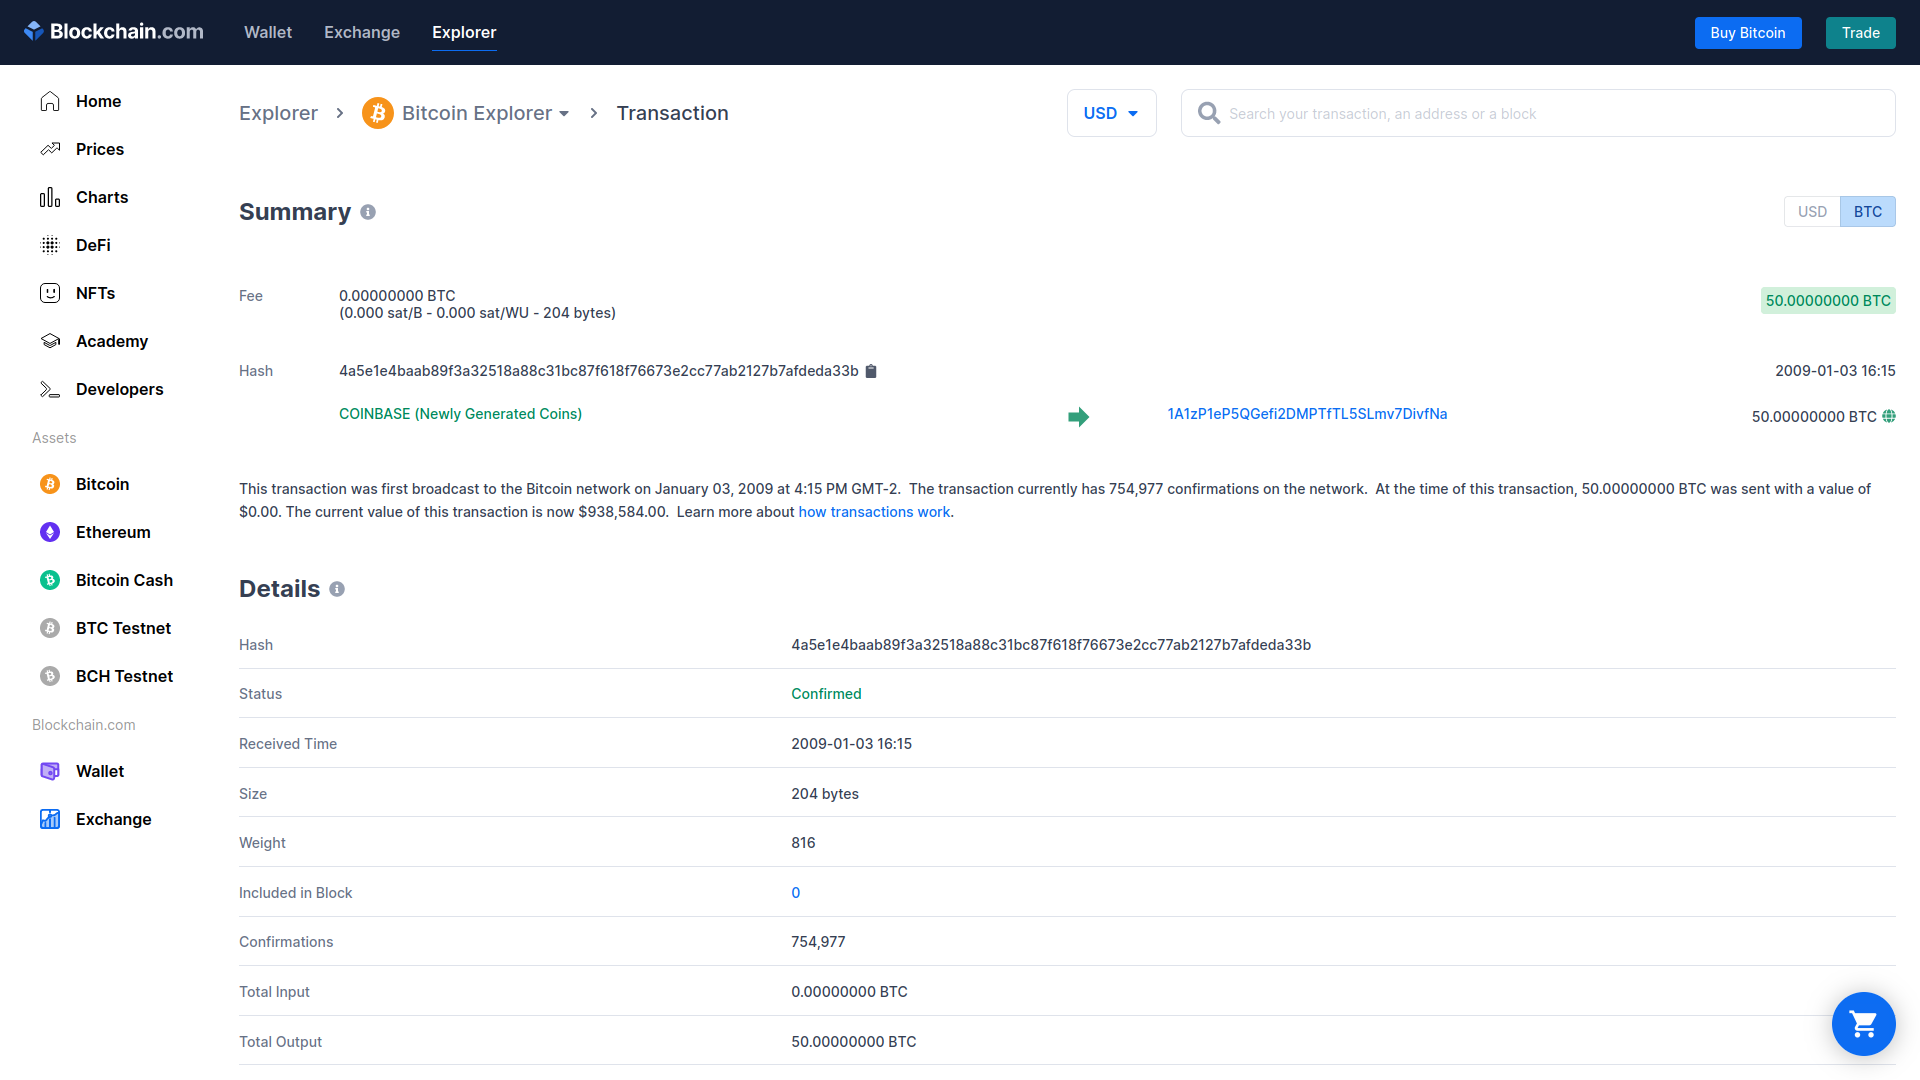
\includegraphics[width=0.9\textwidth,height=\textheight]{figuras/blockchain-com-tx-4a5e1e4baab89f3a32518a88c31bc87f618f76673e2cc77ab2127b7afdeda33b.png}
\caption{\href{https://www.blockchain.com/btc/tx/4a5e1e4baab89f3a32518a88c31bc87f618f76673e2cc77ab2127b7afdeda33b}{4a5e1e4baab89f3a32518a88c31bc87f618f76673e2cc77ab2127b7afdeda33b}}
\end{figure}

\begin{figure}
\centering
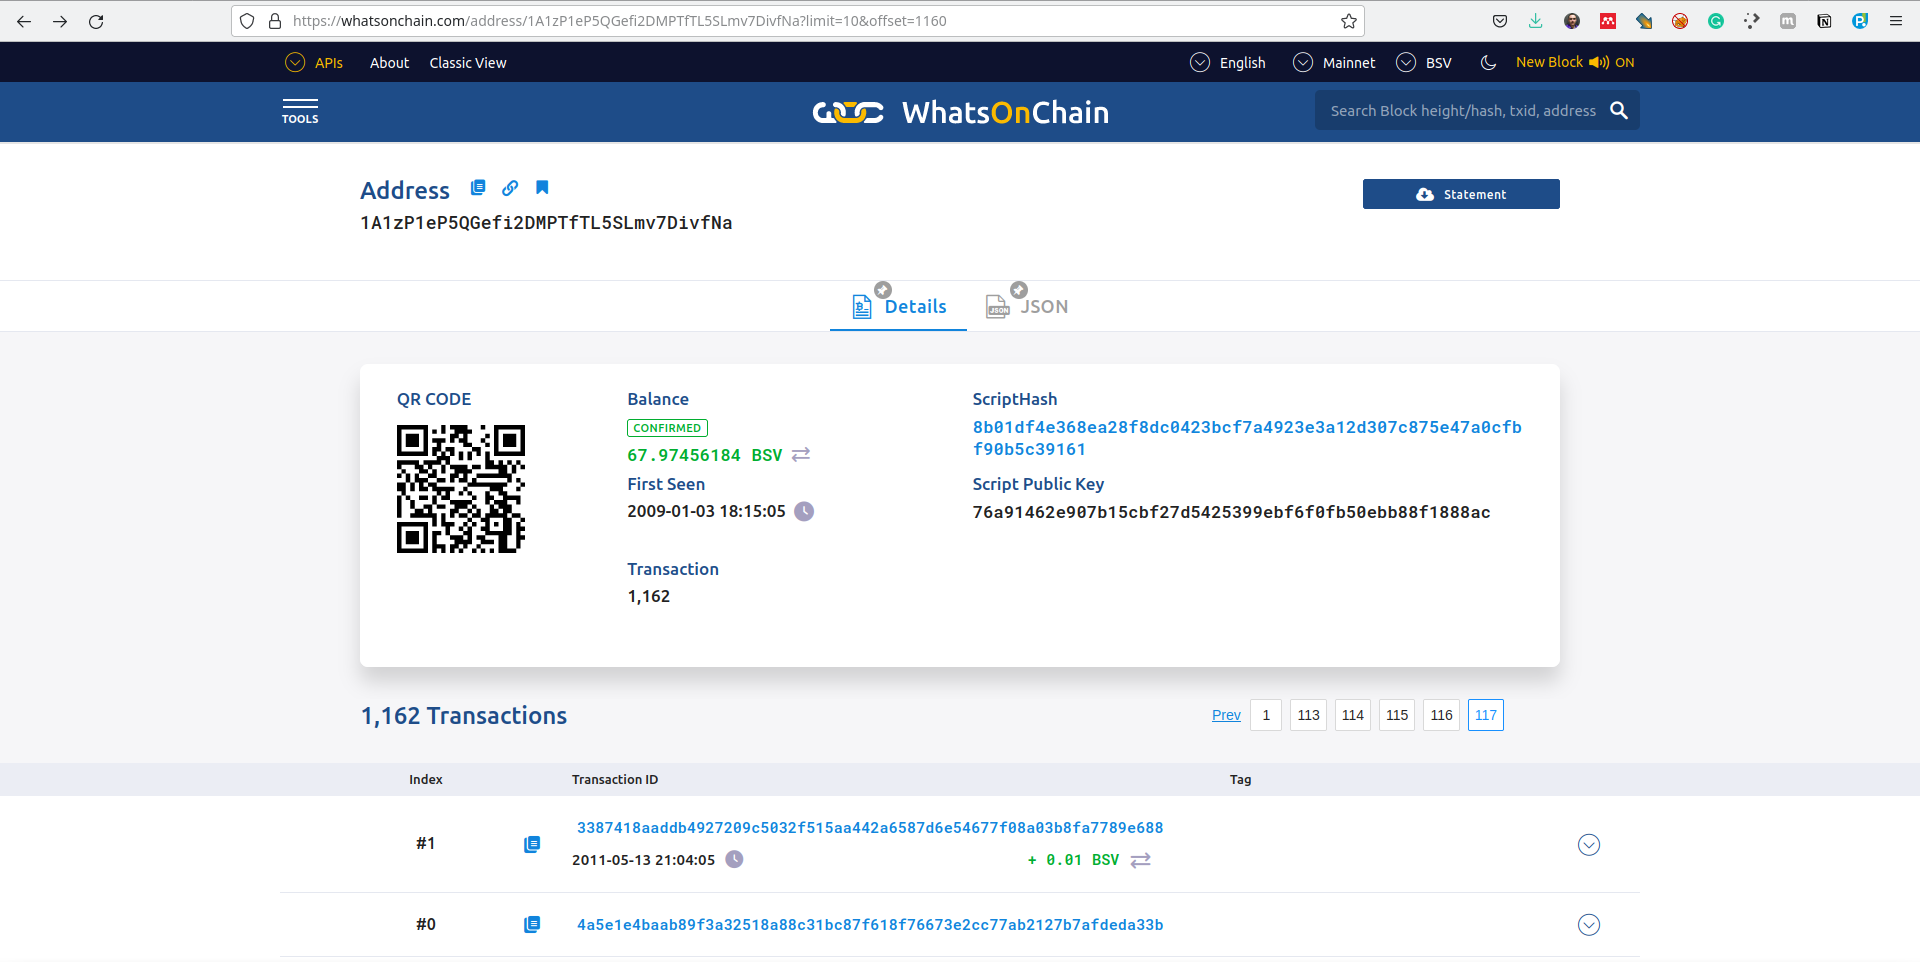
\includegraphics[width=0.9\textwidth,height=\textheight]{figuras/carteira-de-satoshi-1A1zP1eP5QGefi2DMPTfTL5SLmv7DivfNa.png}
\caption{\href{https://whatsonchain.com/address/1A1zP1eP5QGefi2DMPTfTL5SLmv7DivfNa?limit=10\&offset=1160}{1A1zP1eP5QGefi2DMPTfTL5SLmv7DivfNa}}
\end{figure}

\framebreak

\begin{itemize}
\tightlist
\item
  Detalhes da Transação:
\end{itemize}

\begin{figure}
\centering
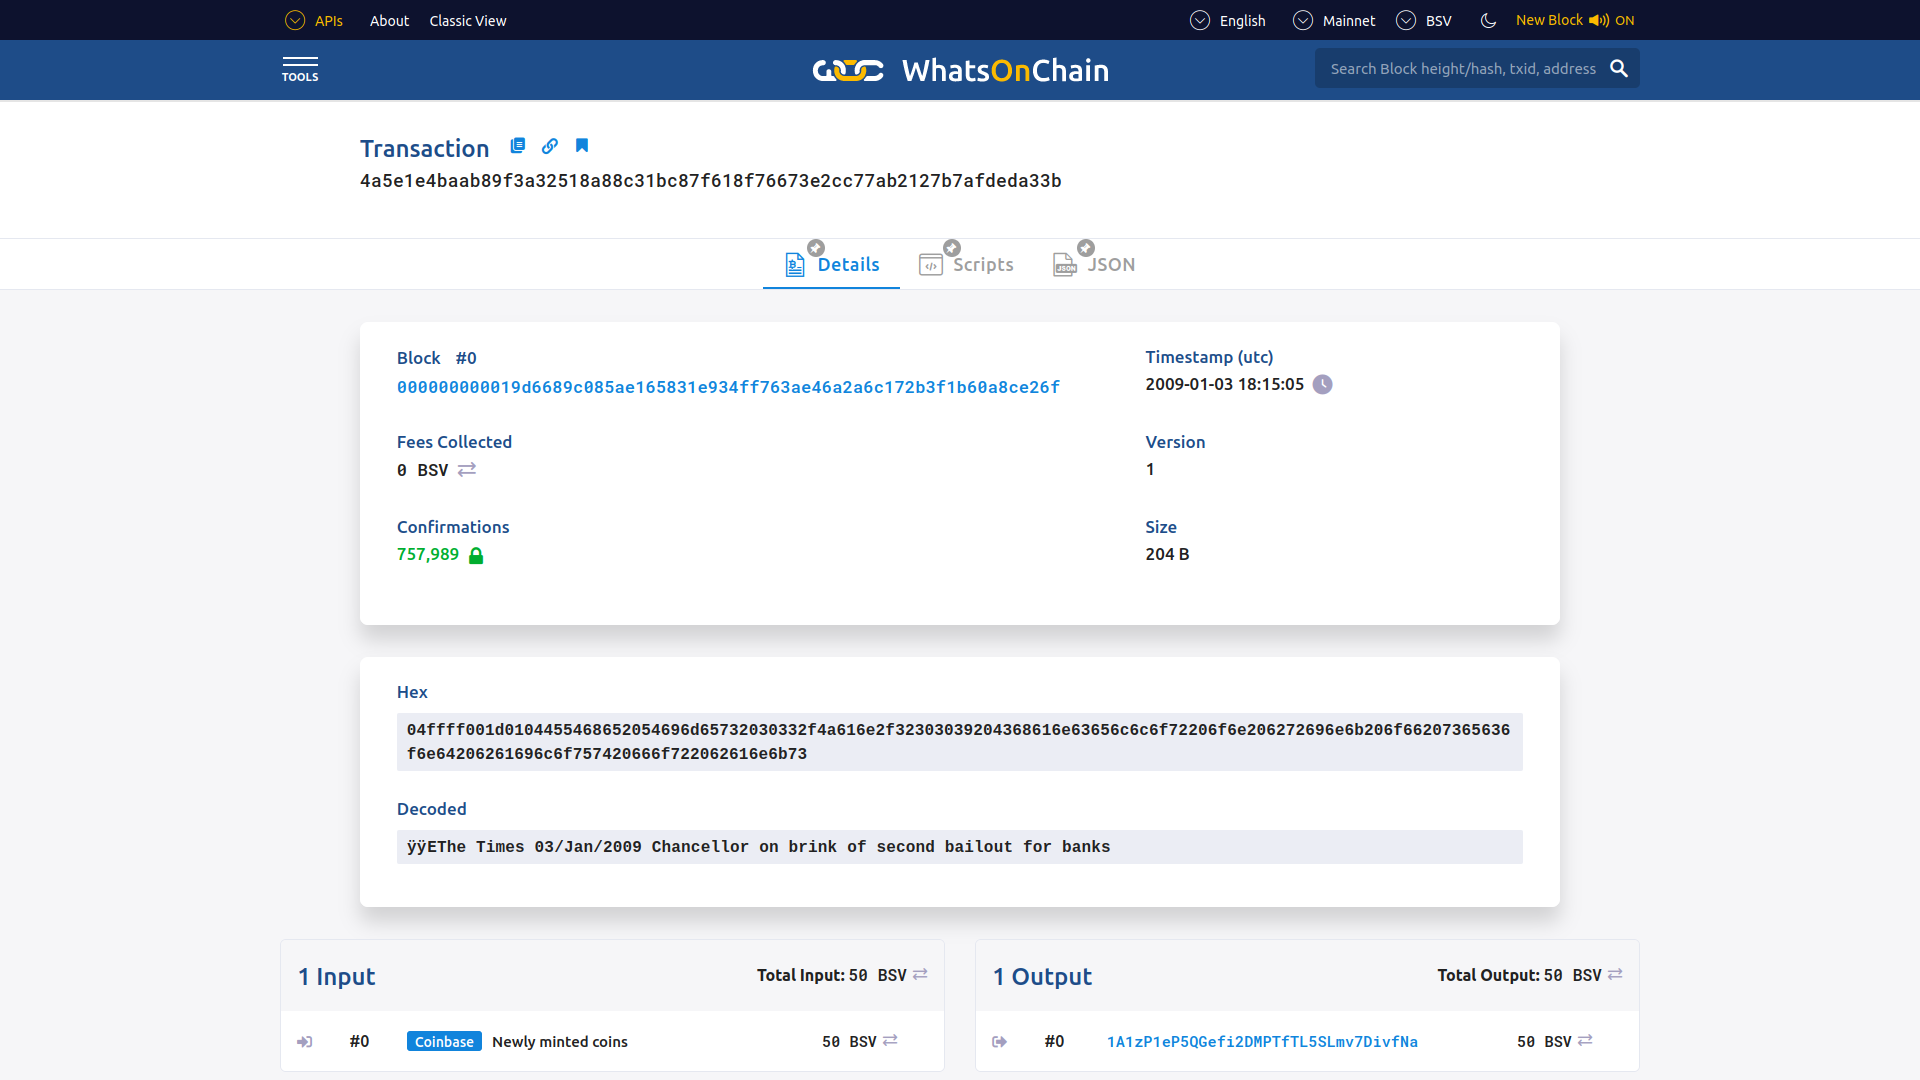
\includegraphics[width=0.9\textwidth,height=\textheight]{figuras/block-0-transaction-4a5e1e4baab89f3a32518a88c31bc87f618f76673e2cc77ab2127b7afdeda33b.png}
\caption{\href{https://whatsonchain.com/tx/4a5e1e4baab89f3a32518a88c31bc87f618f76673e2cc77ab2127b7afdeda33b}{4a5e1e4baab89f3a32518a88c31bc87f618f76673e2cc77ab2127b7afdeda33b}}
\end{figure}

\framebreak

\begin{itemize}
\tightlist
\item
  Scripts
\end{itemize}

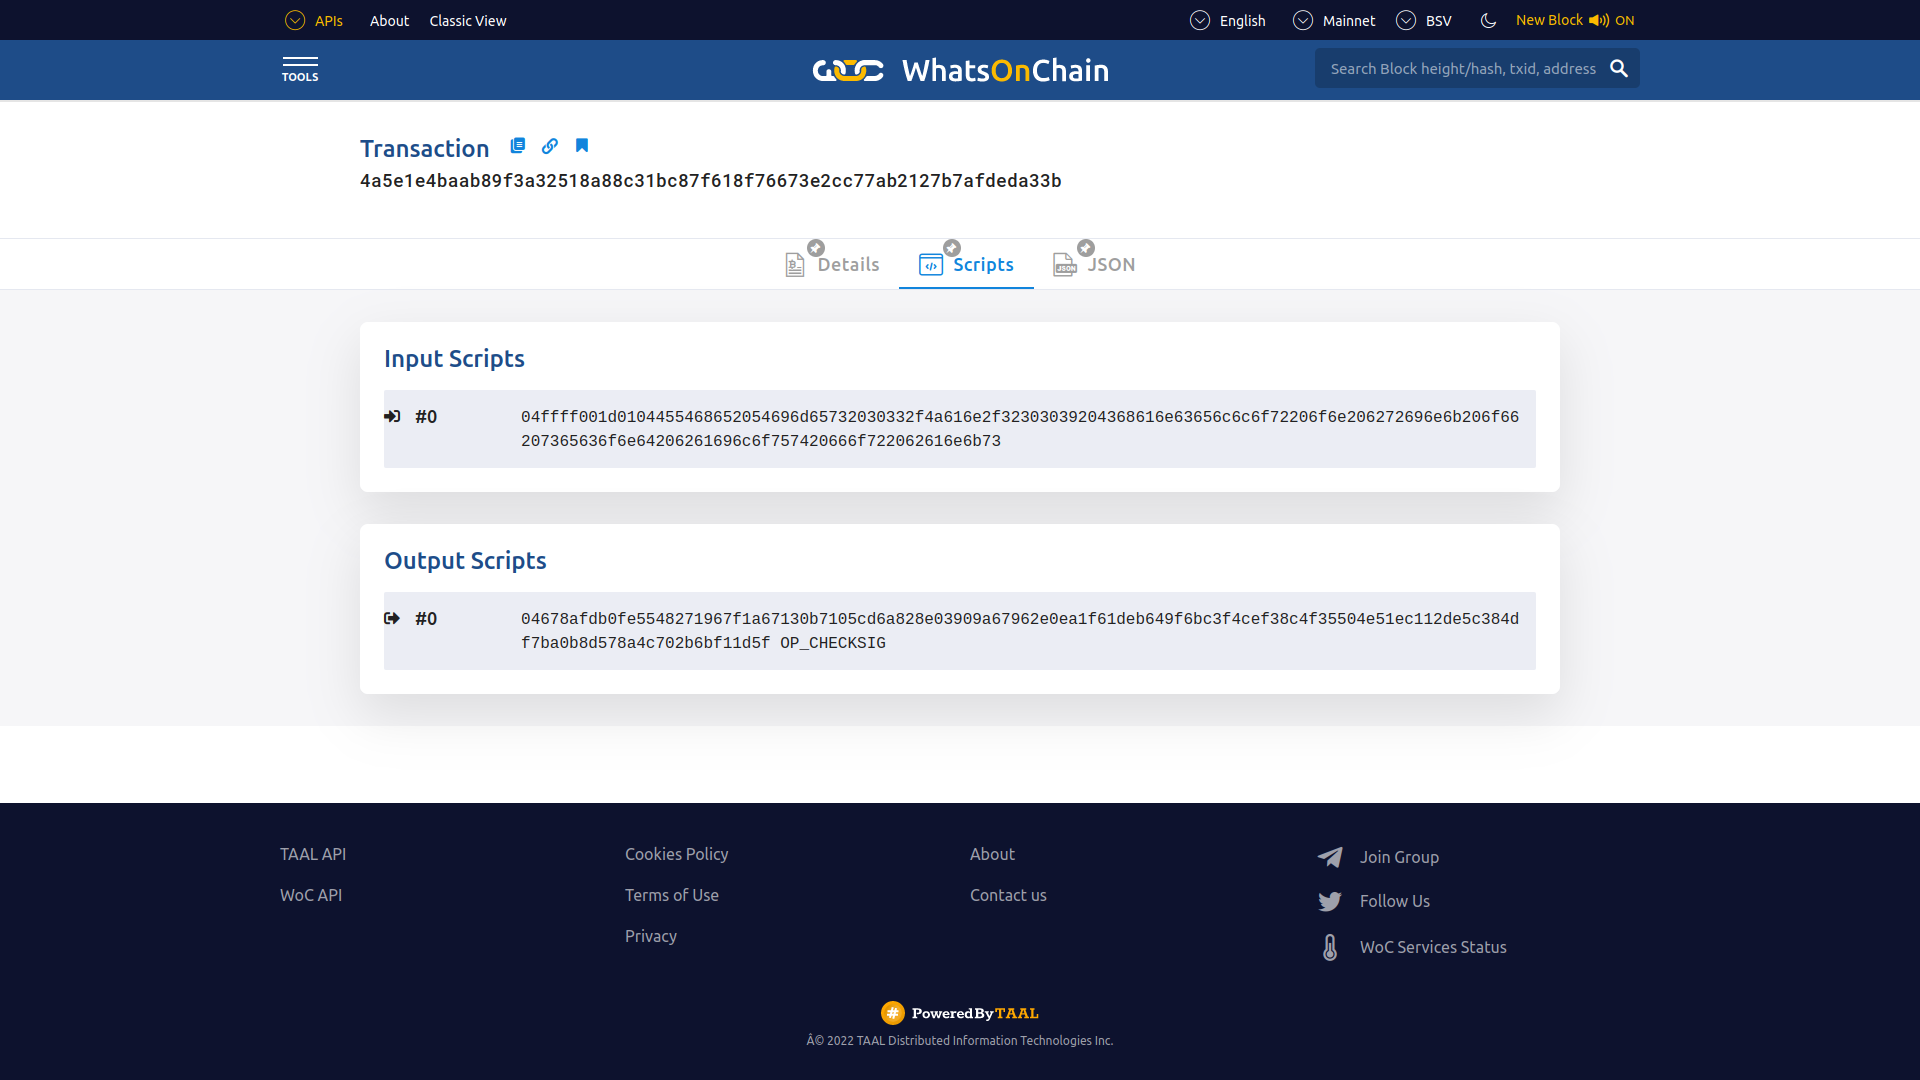
\includegraphics[width=0.9\textwidth,height=\textheight]{figuras/block-0-transaction-4a5e1e4baab89f3a32518a88c31bc87f618f76673e2cc77ab2127b7afdeda33b-scripts.png}

\framebreak

\begin{itemize}
\tightlist
\item
  \texttt{JSON}
\end{itemize}

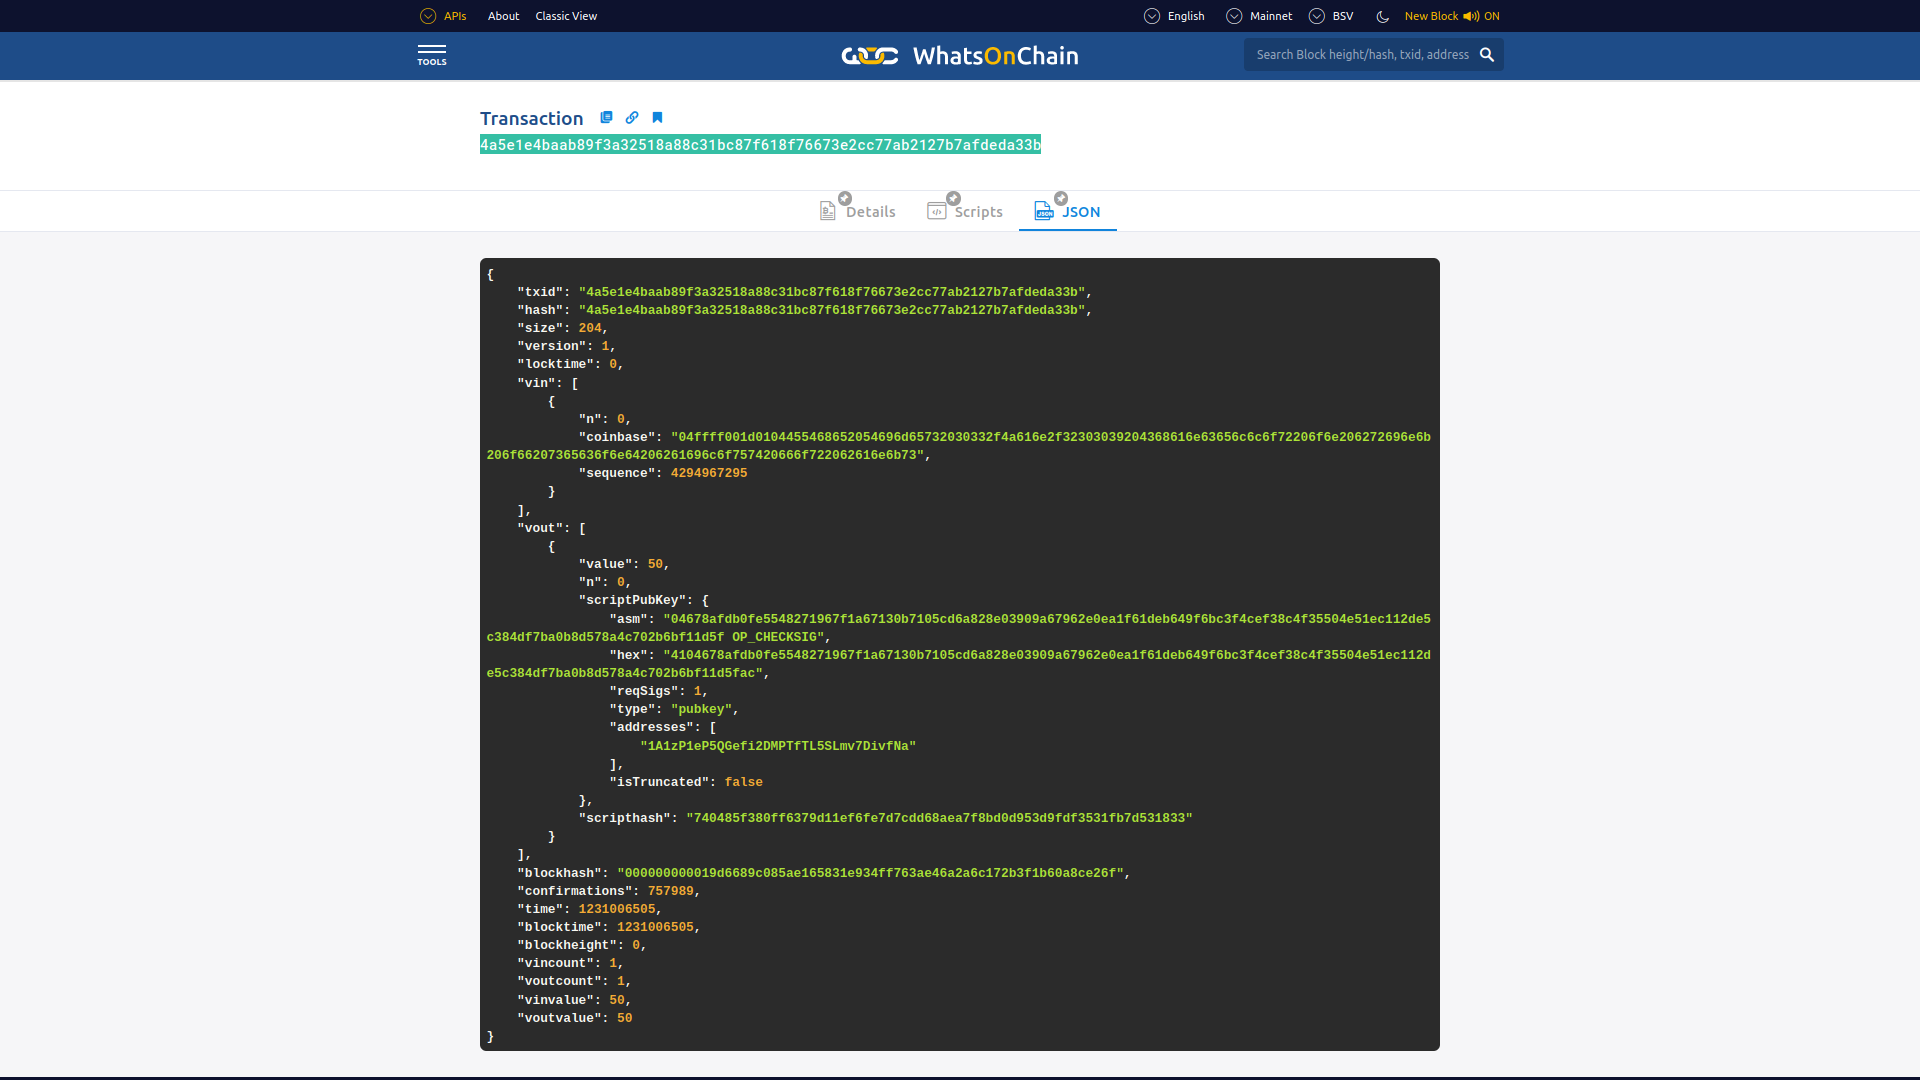
\includegraphics[width=0.9\textwidth,height=\textheight]{figuras/block-0-transaction-4a5e1e4baab89f3a32518a88c31bc87f618f76673e2cc77ab2127b7afdeda33b-json.png}
\end{frame}

\begin{frame}[allowframebreaks]{Blocos Obsoletos e Orfãos}
\protect\hypertarget{blocos-obsoletos-e-orfuxe3os}{}
\begin{itemize}
\tightlist
\item
  Blocos obsoletos existem em uma cadeia mais curta, a partir da qual a
  cadeia principal progrediu.
\item
  Os blocos pais de blocos órfãos são desconhecidos.
\end{itemize}

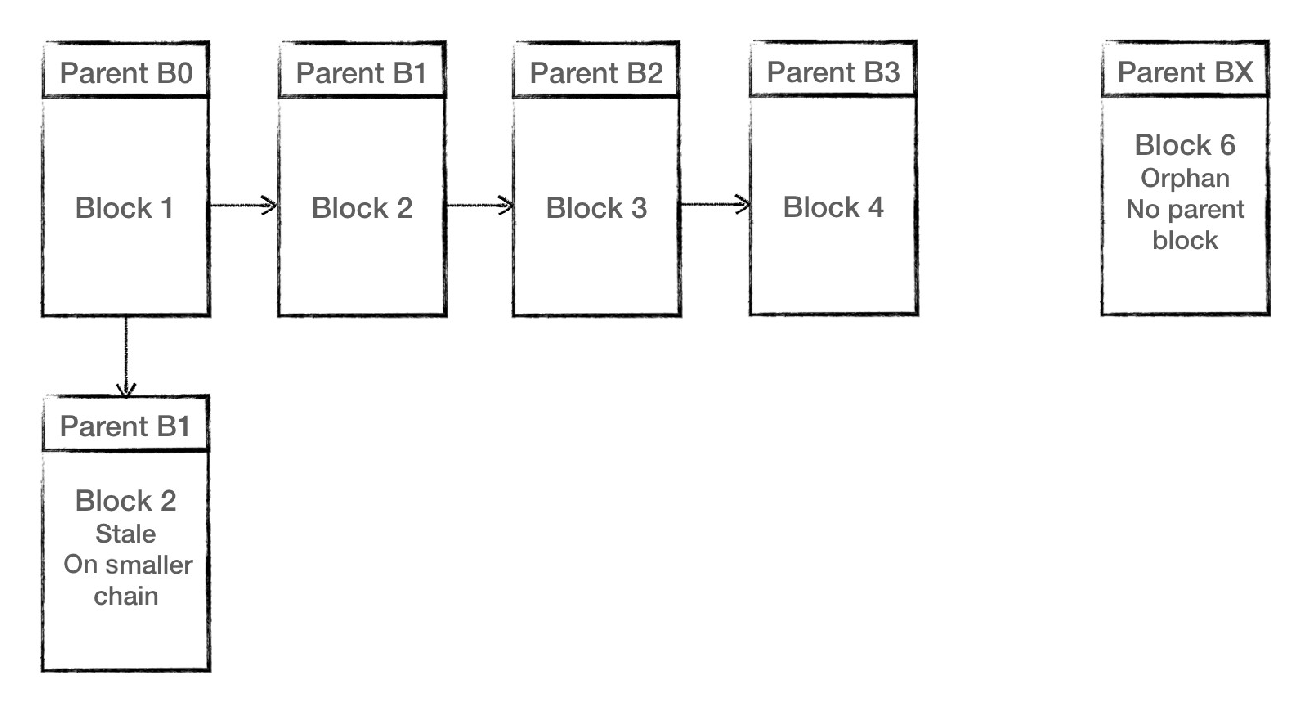
\includegraphics{figuras/bitcoin-blockchain-stale-orphan-blocks.pdf}
\end{frame}

\begin{frame}[allowframebreaks]{Tamanho do Blockchain do Bitcoin}
\protect\hypertarget{tamanho-do-blockchain-do-bitcoin}{}
\begin{itemize}
\tightlist
\item
  O \emph{Blockchain} do \emph{Bitcoin} tinha em \textbf{October 29,
  2017}, aproximadamente: \(139GB\)
\end{itemize}

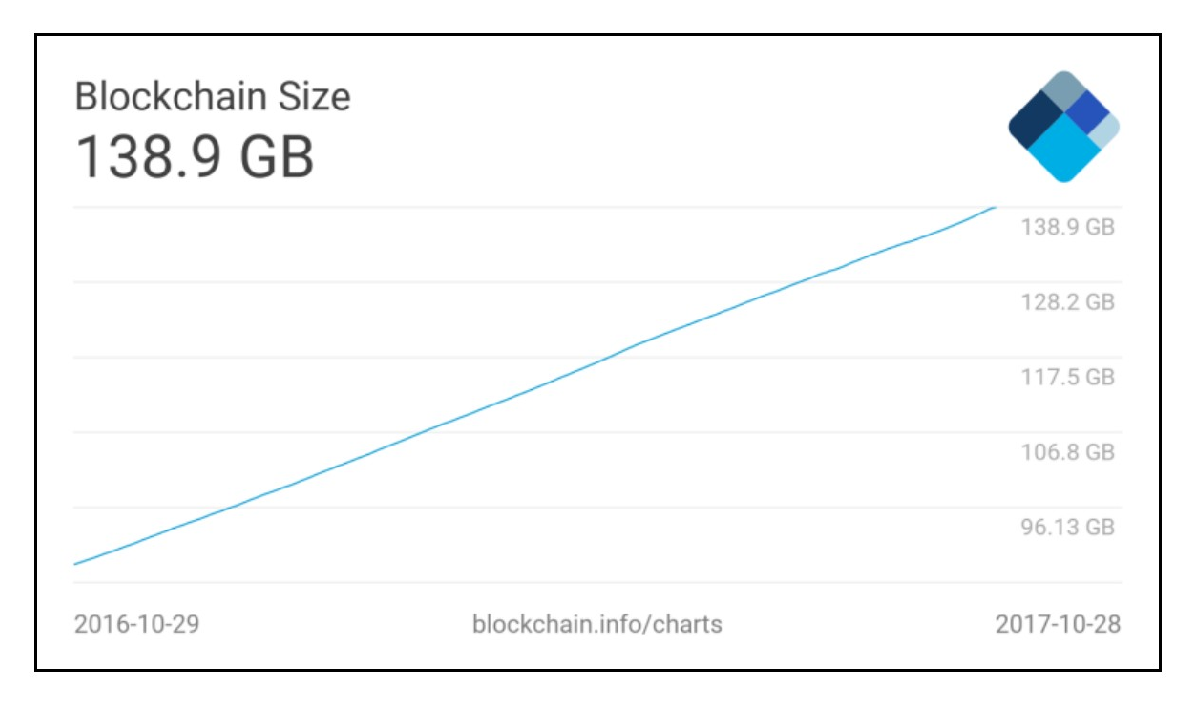
\includegraphics[width=0.75\textwidth,height=\textheight]{figuras/bitcoin-blockchain-size-oct-2017.pdf}

\framebreak

\begin{itemize}
\tightlist
\item
  A figura mostra a evolução de \textbf{Aug 2017} para \textbf{Jul
  2020}. Aproximandamente, \(286GB\).
\end{itemize}

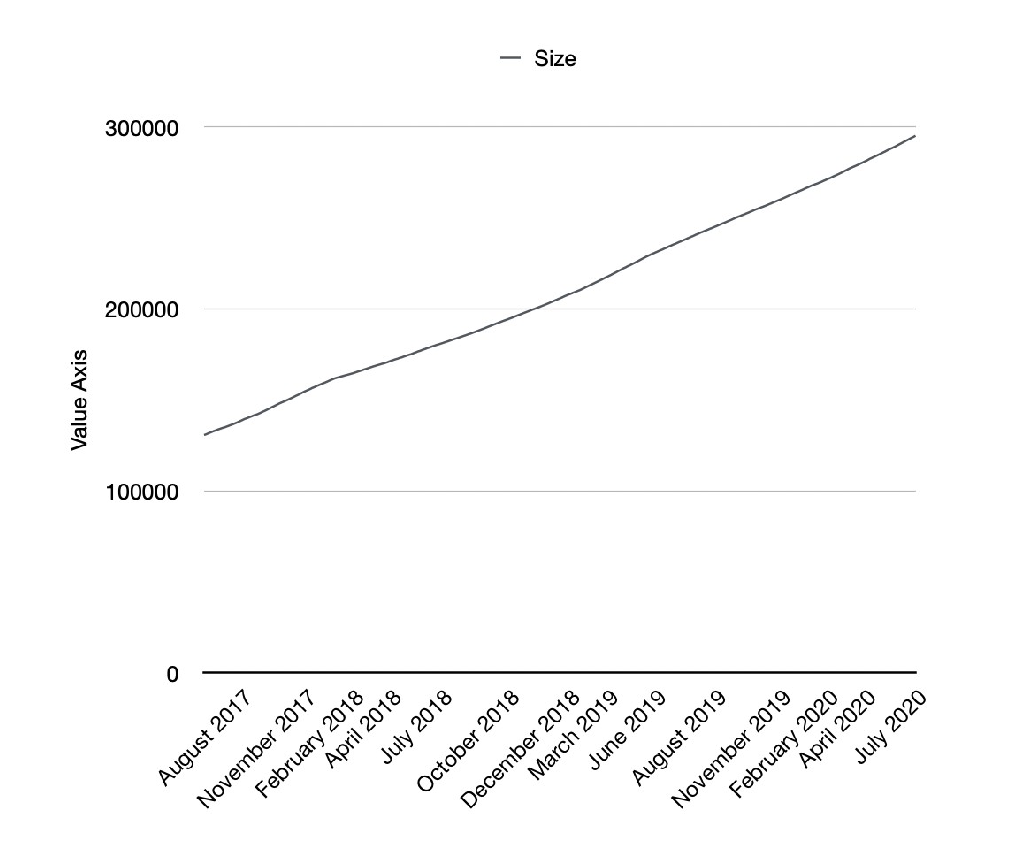
\includegraphics[width=0.6\textwidth,height=\textheight]{figuras/bitcoin-blockchain-size-aug-2017-jul-2020.pdf}

\framebreak

\begin{itemize}
\tightlist
\item
  A figura mostra a evolução de \textbf{Jan 2009} para \textbf{Set
  2022}. Aproximandamente, \(426.7GB\).
\end{itemize}

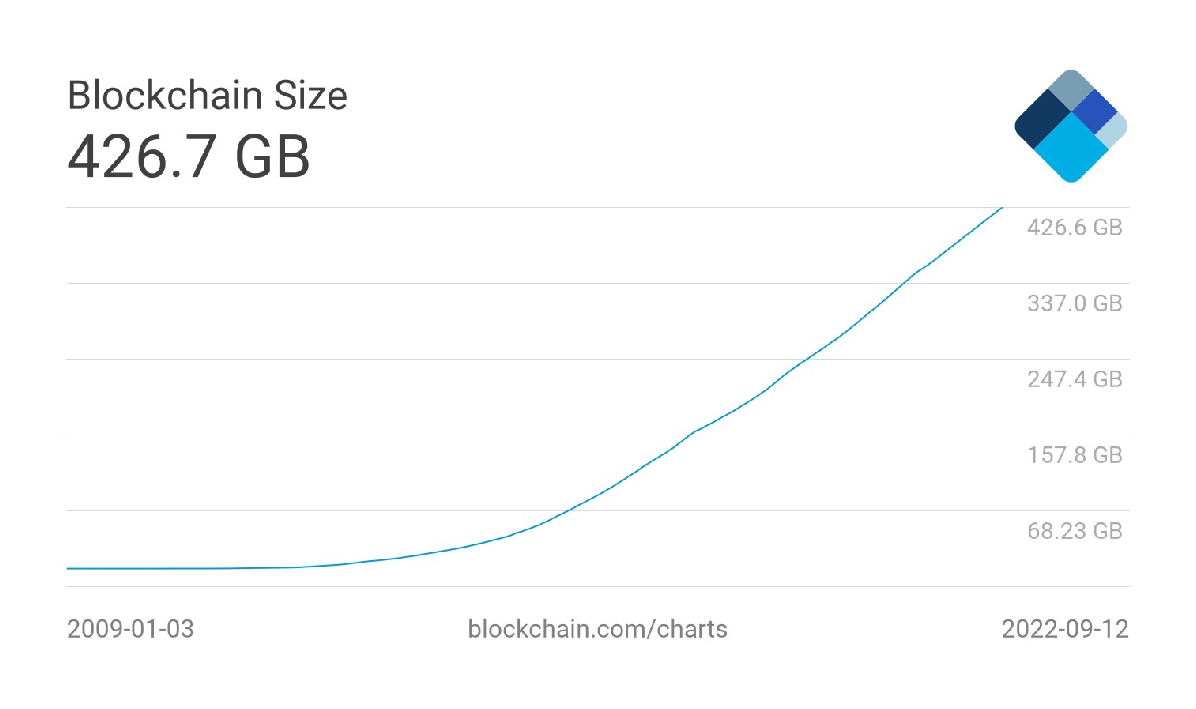
\includegraphics[width=0.75\textwidth,height=\textheight]{figuras/bitcoin-blockchain-size-set-2022.pdf}

\begin{itemize}
\tightlist
\item
  Fonte: \url{https://www.blockchain.com/charts/blocks-size}
\end{itemize}
\end{frame}

\begin{frame}[allowframebreaks]{Mineração}
\protect\hypertarget{minerauxe7uxe3o}{}
\begin{columns}[T]

\column{0.5\textwidth}

\begin{itemize}
\tightlist
\item
  Synchronizing with the network
\item
  Transaction validation
\item
  Block validation
\item
  Create a new block
\item
  Perform PoW
\item
  Fetch reward
\end{itemize}

\column{0.5\textwidth}

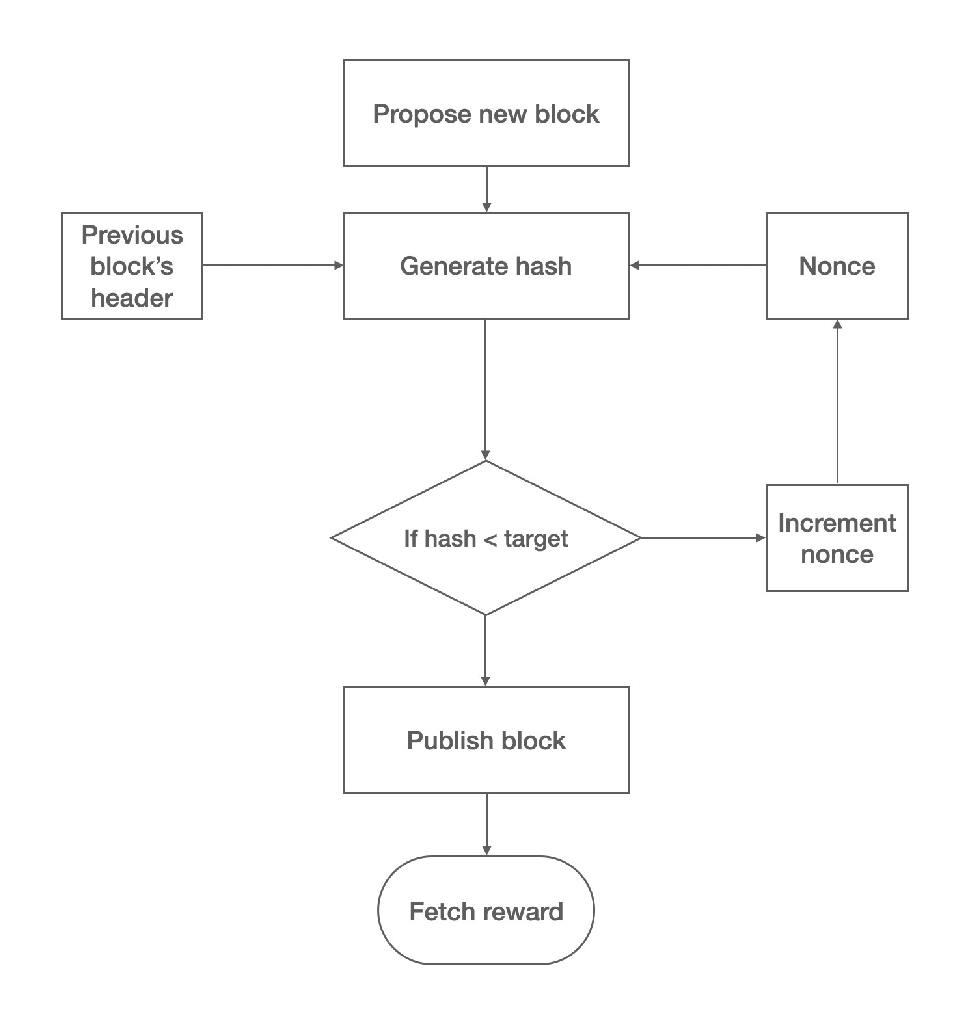
\includegraphics{figuras/mineracao.pdf}

\end{columns}
\end{frame}

\begin{frame}{Mining systems}
\protect\hypertarget{mining-systems}{}
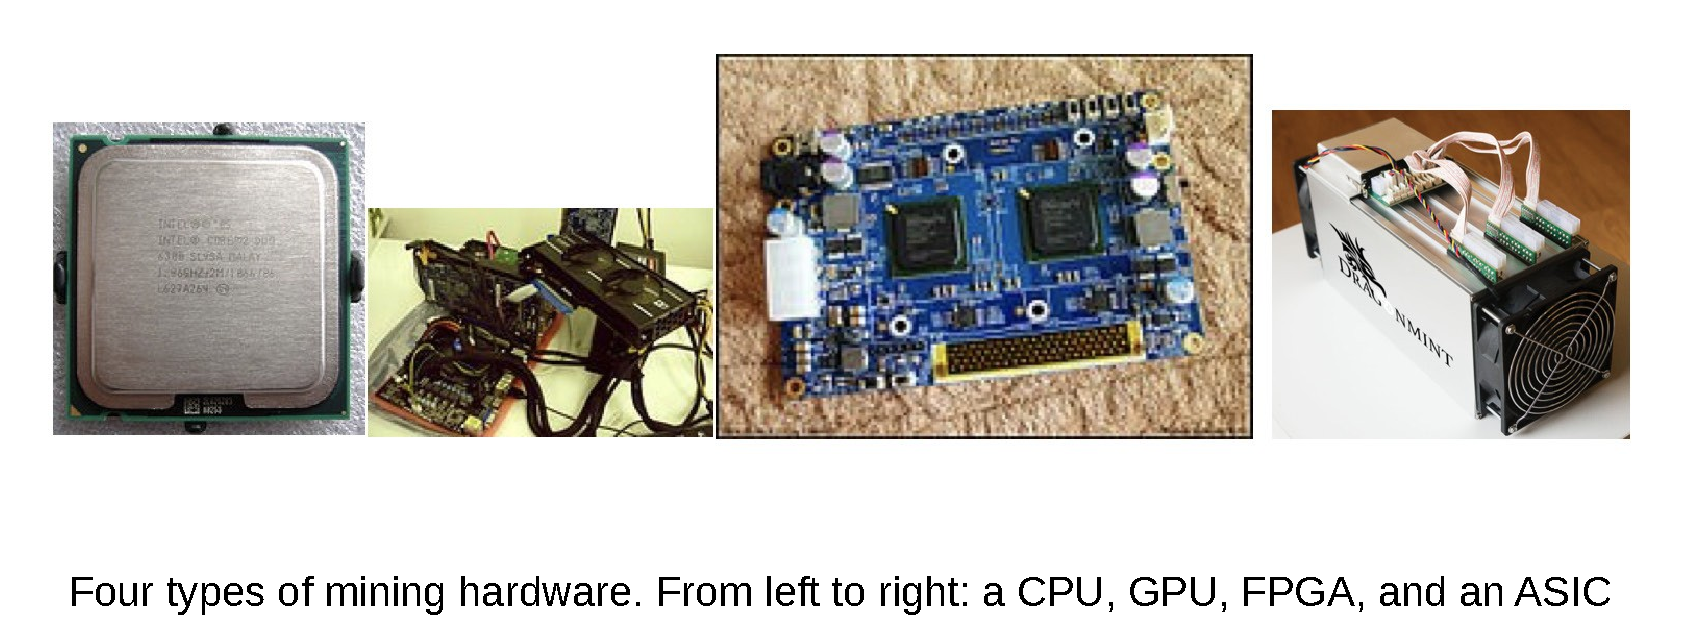
\includegraphics{figuras/sistemas-mineracao.pdf}
\end{frame}

\begin{frame}{Atividade}
\protect\hypertarget{atividade-1}{}
\begin{itemize}
\tightlist
\item
  Instalar o Bitcoin client e executar experimentos nele.
\end{itemize}
\end{frame}

\begin{frame}{Leitura Recomendada}
\protect\hypertarget{leitura-recomendada-1}{}
\normalsize

\begin{alertblock}{Leitura Recomendada}

\textbf{Capítulo 5/6: Introduction Bitcoin}

\textbf{Livro}:
\href{https://search.ebscohost.com/login.aspx?direct=true\&db=e000xww\&AN=1789486\&authtype=shib\&lang=pt-br\&site=eds-live\&scope=site\&ebv=EB\&ppid=pp_129}{IMRAN
BASHIR. Mastering Blockchain\,: Distributed Ledger Technology,
Decentralization, and Smart Contracts Explained, 2nd Edition.}

\end{alertblock}
\end{frame}

\hypertarget{smart-contracts-contratos-inteligentes}{%
\section{Smart Contracts (Contratos
Inteligentes)}\label{smart-contracts-contratos-inteligentes}}

\begin{frame}{Contratos Inteligentes}
\protect\hypertarget{contratos-inteligentes}{}
\begin{itemize}
\item
  Colocar definição
\item
  Falar o que são
\item
  Uso e utilidade
\item
  Citando o artigo original
\item
  Artigo Seminal
\end{itemize}

\begin{alertblock}{Leitura Recomendada}

\begin{block}{Leitura do Capítulo 9/10: \emph{Smart Contracts}}
\protect\hypertarget{leitura-do-capuxedtulo-910-smart-contracts}{}
\begin{enumerate}
\tightlist
\item
  Faça a leitura do
  \href{https://search.ebscohost.com/login.aspx?direct=true\&db=e000xww\&AN=1789486\&lang=pt-br\&site=eds-live\&scope=site\&ebv=EB\&ppid=pp_261}{Capítulo
  9/10: Smart Contracts}
\end{enumerate}

\end{alertblock}
\end{block}
\end{frame}

\hypertarget{ethereum}{%
\section{Ethereum}\label{ethereum}}

\begin{frame}[allowframebreaks]{Ethereum -- Overview}
\protect\hypertarget{ethereum-overview}{}
\begin{itemize}
\tightlist
\item
  Vitalik Buterin (https://vitalik.ca) conceitualizou Ethereum
  (https://ethereum.org) em Novembro de 2013.
\item
  A ideia central proposta foi o desenvolvimento de uma linguagem
  \textbf{Turing-completa} para permitir o desenvolvimento de programas
  arbitrários (contratos inteligentes) para \emph{blockchain} e
  Aplicações Descentralizados (DApps).
\item
  Este conceito difere do \emph{Bitcoin}, onde a linguagem de
  \textbf{script} é limitada e permite apenas as operações necessárias.
\end{itemize}

\begin{figure}
\centering
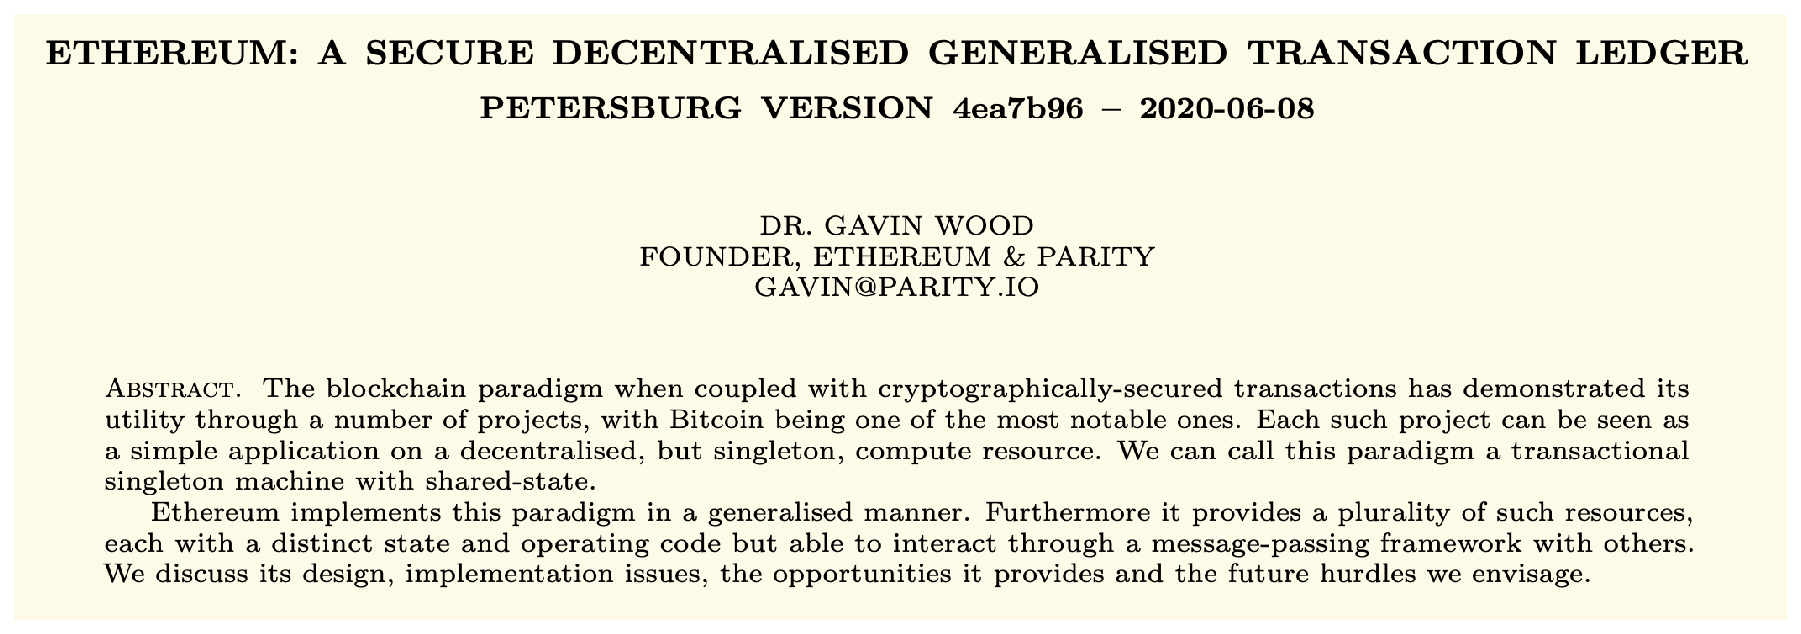
\includegraphics{figuras/yellow-paper.pdf}
\caption[O
\href{https://ethereum.github.io/yellowpaper/paper.pdf}{\emph{Ethereum
Yellow Paper}}]{O
\href{https://ethereum.github.io/yellowpaper/paper.pdf}{\emph{Ethereum
Yellow Paper}\footnotemark{}}}
\end{figure}
\footnotetext{\url{http://ethdocs.org/en/latest/contracts-and-transactions/developer-tools.html\#developer-tools}}

\framebreak

\begin{itemize}
\tightlist
\item
  O
  \href{https://ethereum.github.io/yellowpaper/paper.pdf}{\emph{Ethereum
  Yellow Paper}} foi escrito por Dr.~Gavin Wood, o fundador do
  \emph{Ethereum} e da Parity (\url{http://gavwood.com}), e serve como
  uma especificação formal do protocolo da \emph{Ethereum}.
\item
  Qualquer pessoa pode implementar um cliente Ethereum seguindo as
  especificações de protocolo definidas no artigo.
\end{itemize}
\end{frame}

\begin{frame}[allowframebreaks]{Ethereum Releases}
\protect\hypertarget{ethereum-releases}{}
\begin{itemize}
\item
  A primeira versão da \emph{Ethereum}, denominada \textbf{Olympic}, foi
  liberada em Maio de 2015. Dois meses mais tarde, a versão chamada de
  \textbf{Frontier} foi liberada em Julho. Outra versão, a
  \textbf{Homestead} com várias melhorias foi liberada em Março de 2016.
  A release chamada de \textbf{Muir Glacier}, que atrasou a
  \textbf{difficulty bomb} (https://eips.ethereum.org/EIPS/eip-2384). Um
  grande lançamento antes disso foi Istambul, que incluiu mudanças em
  torno de privacidade e dimensionamento capacidades.
\item
  Uma lista de todas as \emph{releases} anunciadas é mantida em
  \url{https://github.com/ethereum/go-ethereum/releases}.
\end{itemize}
\end{frame}

\begin{frame}[allowframebreaks]{A Blockchain Ethereum}
\protect\hypertarget{a-blockchain-ethereum}{}
\begin{itemize}
\tightlist
\item
  O Ethereum, assim como qualquer outro \emph{blockchain}, pode ser
  visualizado como uma máquina de estado baseada em transações.
\end{itemize}

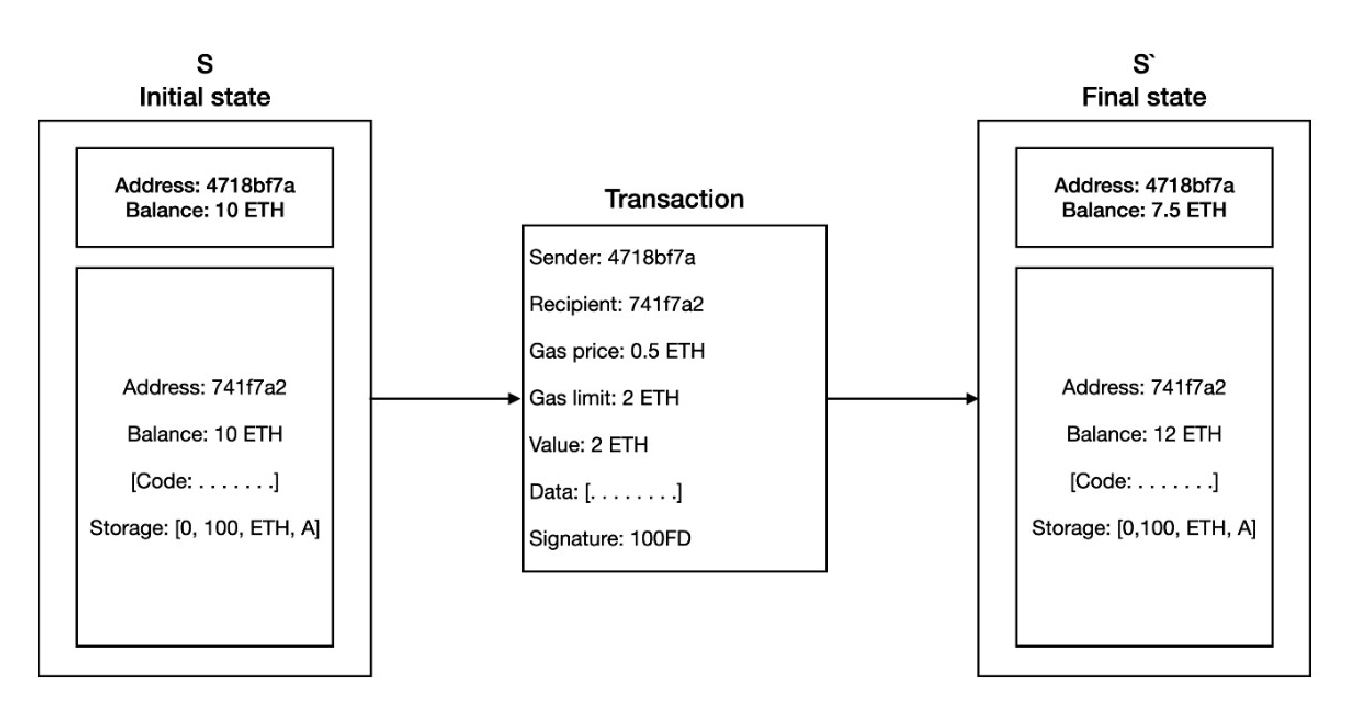
\includegraphics{figuras/ethereum-blockchain.pdf}

\begin{itemize}
\tightlist
\item
  A ideia principal da \emph{blockchain} da \emph{Ethereum}, um estado
  gênese é transformado em um estado final executando transações de
  forma incremental. A transformação final é então aceita como a versão
  absoluta e indiscutível do estado. A função de transição de estado
  \emph{Ethereum} é mostrada, onde a execução de uma transação resultou
  em uma transição de estado.
\end{itemize}
\end{frame}

\begin{frame}[allowframebreaks]{Ethereum -- a user's perspective~}
\protect\hypertarget{ethereum-a-users-perspective}{}
\begin{itemize}
\tightlist
\item
  O caso de uso mais comum do rede \emph{Ethereum} é o envio e o
  recebimento de pagamentos.
\item
  Para isso, o usuário assina a transação e a envia, que se propaga na
  rede, momento em que os mineradores a pegam, verificam e iniciam a
  Prova de Trabalho (PoW).
\item
  Se PoW for bem sucedida, o bloco com a transação é finalizado e
  propagado, e um novo bloco é adicionado à cadeia
\item
  Para enviar e receber transações, um software de carteira é usado: por
  exemplo, carteiras são usadas em dispositivos móveis.
\end{itemize}
\end{frame}

\begin{frame}[allowframebreaks]{Arquitetura de Alto Nível da Ethereum}
\protect\hypertarget{arquitetura-de-alto-nuxedvel-da-ethereum}{}
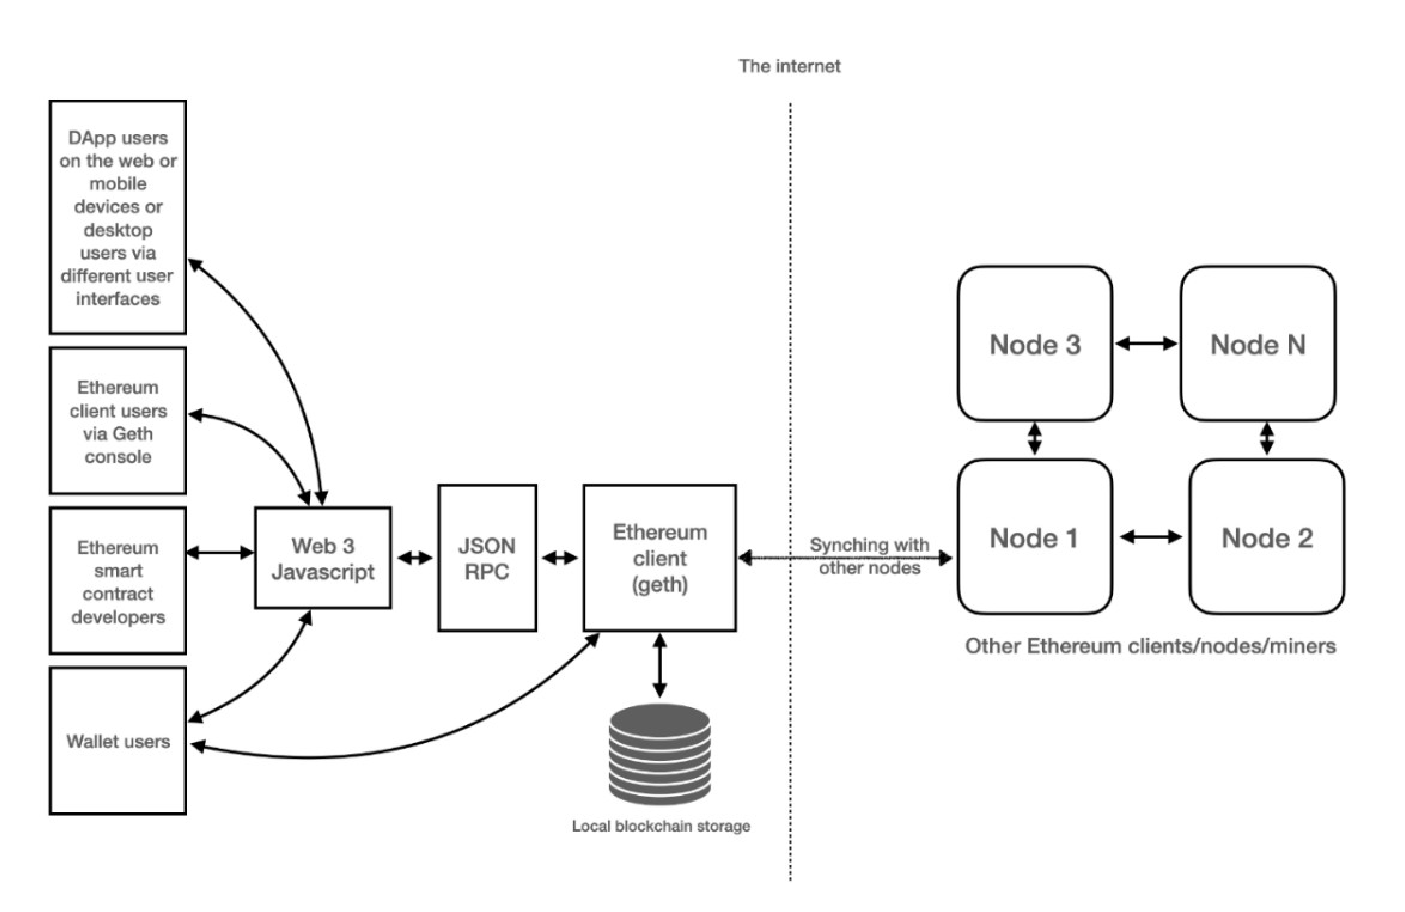
\includegraphics{figuras/ethereum-high-level-architecture.pdf}
\end{frame}

\begin{frame}[fragile,allowframebreaks]{Rede Ethereum}
\protect\hypertarget{rede-ethereum}{}
A rede \emph{Ethereum} é uma rede \emph{peer-to-peer} onde os nós
participantes mantem a \emph{blockchain} e contribuem para o mecanismo
de consenso. As redes podem ser divididas em três tipos, com base nos
requisitos e uso.

\begin{block}{A mainnet}

A \textbf{mainnet} é a atual rede \emph{Ethereum}. Seu ID de rede é
\(1\) e seu ID de cadeia (\emph{chain}) é também \(1\). Os IDs de rede e
de cadeia são usados para identificar a rede. Um explorador de blocos
que mostra informações detalhadas sobre blocos e outras métricas
relevantes estão disponíveis em \url{https://etherscan.io}, que pode ser
usado para explorar a blockchain Ethereum.

\end{block}

\begin{alertblock}{Testnets}

Existem um número de redes de testes (testnets) disponíveis para
\emph{Ethereum}. Elas tem como objetivo fornecer um ambiente de testes
para contratos inteligentes e DApps antes de serem implantados para
produção na rede \emph{blockchain}. Além disso, sendo redes de teste,
elas permitem experimentos e pesquisa. A principal testnet é chamada
\texttt{Ropsten}, que contém todas as características de outras redes de
propósito especial menores que foram criados para fins específicos. Por
exemplo, outras redes de teste incluem \texttt{Kovan} e
\texttt{Rinkeby}, que foram desenvolvidos para testar as versões do
\textbf{Byzantium}. As mudanças que foram implementados nessas redes de
teste menores também foram implementados em \texttt{Ropsten}. Agora a
rede de teste \texttt{Ropsten} contém todas as propriedades de
\texttt{Kovan} e \texttt{Rinkeby}.

\end{alertblock}

\begin{exampleblock}{Redes Privadas}

As \emph{private nets} são redes privadas que podem ser criadas
gerando-se um novo \emph{genesis block}. Este é geralmente o caso em
redes \emph{blockchain} privadas, onde um grupo privado de entidades
iniciam sua rede \emph{blockchain} e a usam como uma blockchain
autorizada ou de consórcio.

\end{exampleblock}
\end{frame}

\begin{frame}[allowframebreaks]{Elementos do Ecossistema Ethereum}
\protect\hypertarget{elementos-do-ecossistema-ethereum}{}
\begin{itemize}
\tightlist
\item
  Chaves e Endereços
\item
  Contas
\item
  Transações e mensagens
\item
  Criptomoeda/Tokens Ether
\item
  A Ethereum Virtual Machine (EVM)~
\item
  Smart contracts e contratos nativos.
\end{itemize}
\end{frame}

\begin{frame}[allowframebreaks]{Tipos de contas}
\protect\hypertarget{tipos-de-contas}{}
\begin{itemize}
\tightlist
\item
  \textbf{EOAs:} \emph{Externally Owned Accounts}. Contas de usuários
  representadas por um endereço.
\item
  \textbf{CAs:} \emph{Contract accounts}. Criadas como resultado do
  \emph{deployment} de um contrato inteligente, também representado por
  um endereço.
\end{itemize}
\end{frame}

\begin{frame}[allowframebreaks]{Transações e Árvore de Transações
(trie)}
\protect\hypertarget{transauxe7uxf5es-e-uxe1rvore-de-transauxe7uxf5es-trie}{}
\begin{alertblock}{Transações}

Uma transação no \emph{Ethereum} consiste em vários campos, como
mostrado aqui, junto com a \emph{transaction trie}. O diagrama também
mostra a relação entre a tentativa de transação e o cabeçalho do bloco.

\end{alertblock}

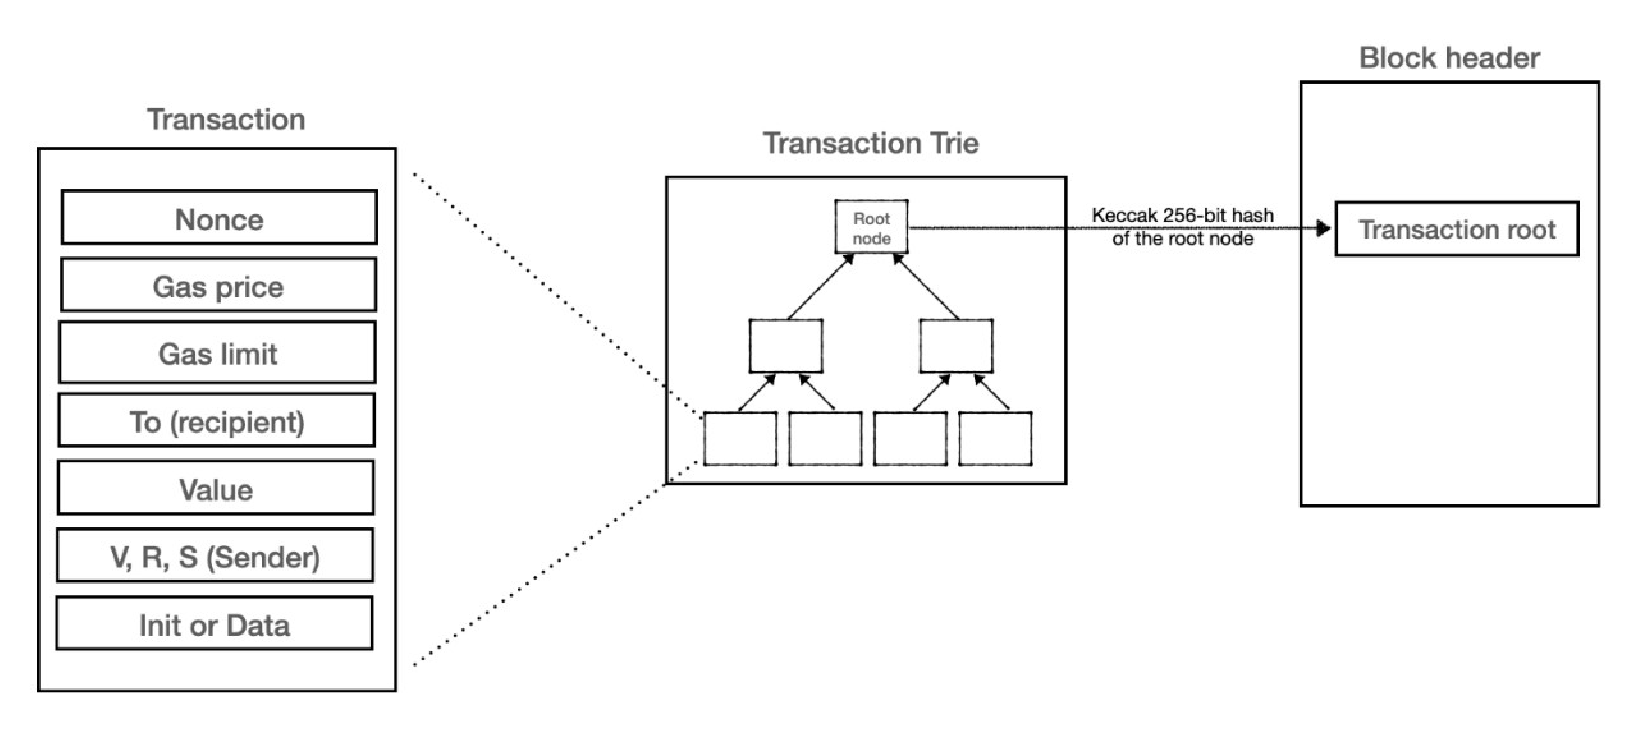
\includegraphics{figuras/ethereum-transaction-trie.pdf}
\end{frame}

\begin{frame}[allowframebreaks]{Tipos de Transações}
\protect\hypertarget{tipos-de-transauxe7uxf5es}{}
\begin{itemize}
\tightlist
\item
  Existem três tipo de transações:

  \begin{itemize}
  \tightlist
  \item
    Criação de Contrato
  \item
    \emph{Call}
  \item
    Transferência de Valor
  \end{itemize}
\end{itemize}

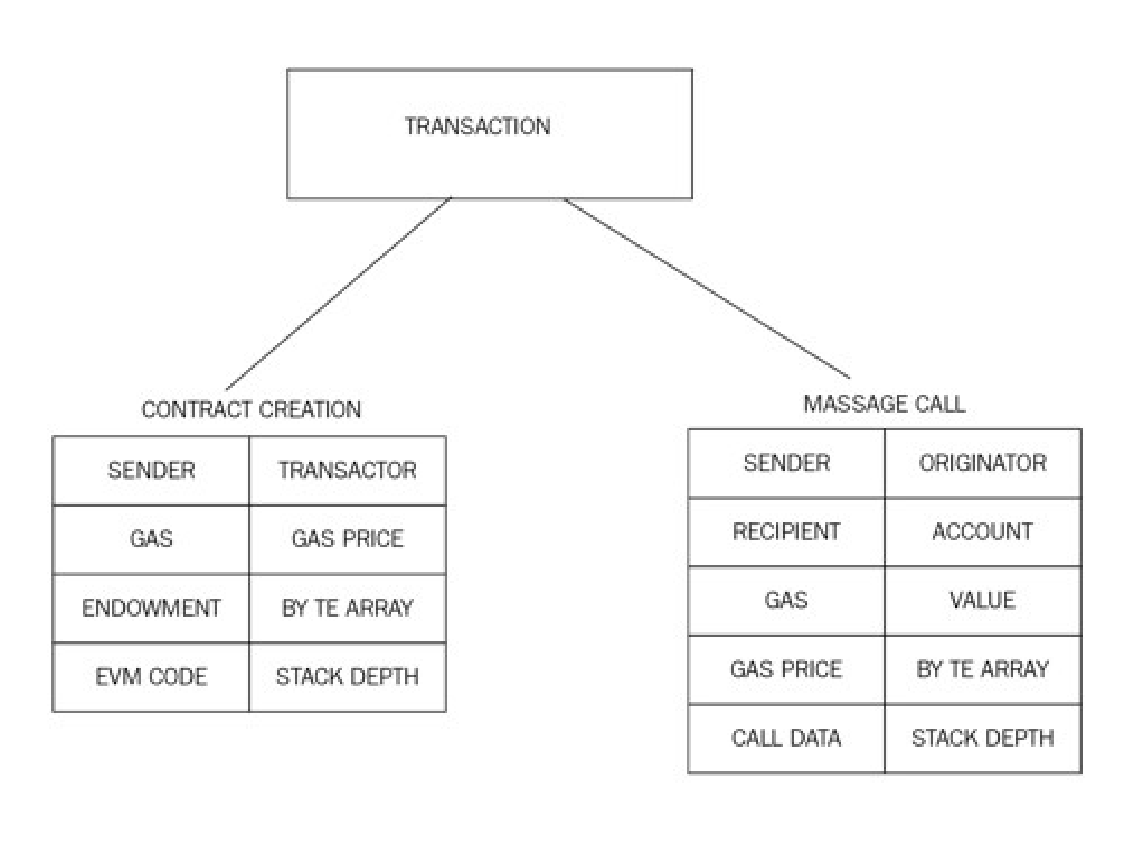
\includegraphics{figuras/ethereum-transaction.pdf}

O diagrama mostra a criação do contrato e as transações de chamada de
mensagem, com campos obrigatórios.
\end{frame}

\begin{frame}[allowframebreaks]{Estado da conta e armazenamento na trie}
\protect\hypertarget{estado-da-conta-e-armazenamento-na-trie}{}
O diagrama mostra os campos contidos no estado da conta e como os vários
elementos estão contidos no \emph{world state} trie: * World state trie
* State root * Account state * Account storage trie

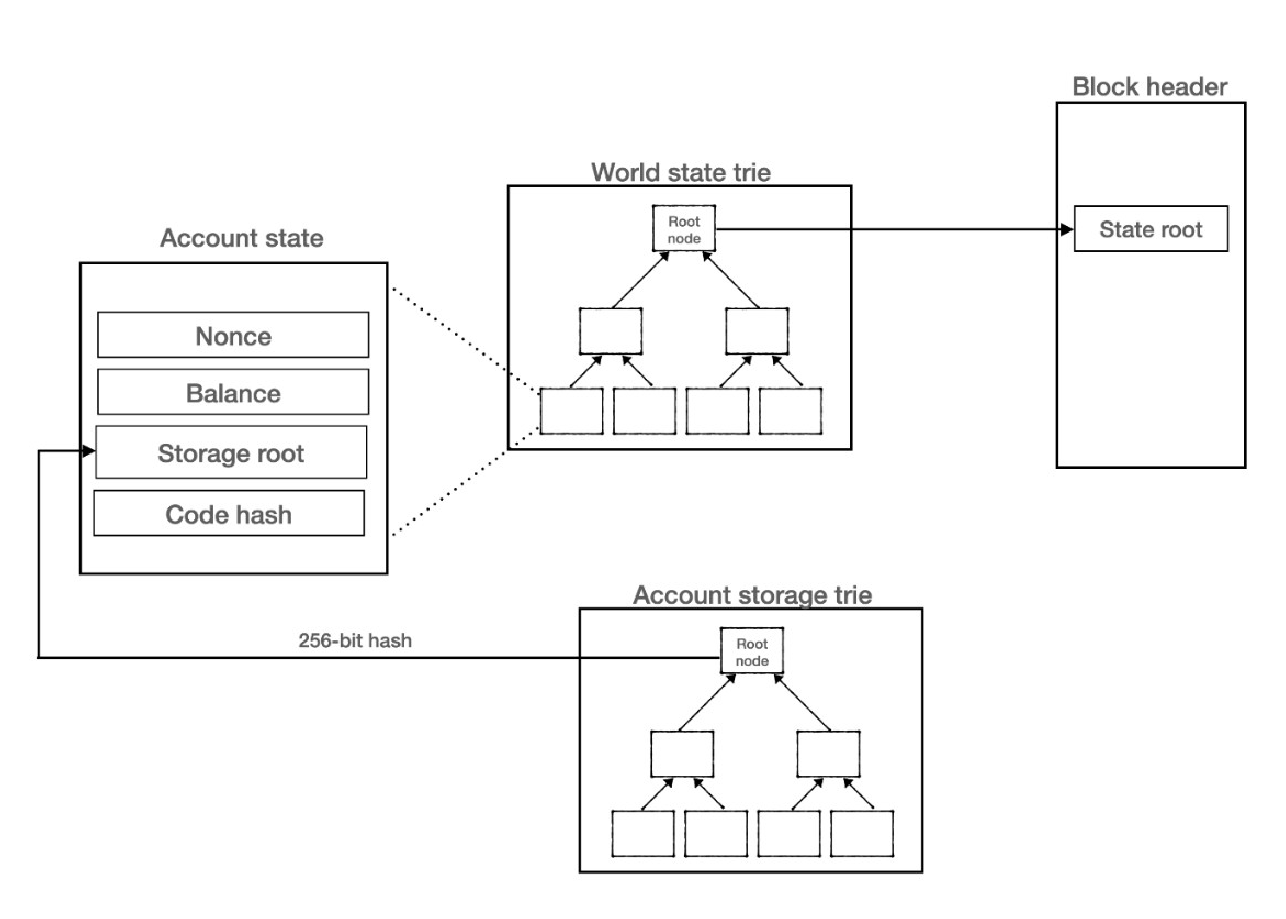
\includegraphics{figuras/ethereum-account-state-storage.pdf}
\end{frame}

\begin{frame}[allowframebreaks]{Recibos de Transações}
\protect\hypertarget{recibos-de-transauxe7uxf5es}{}
\begin{itemize}
\tightlist
\item
  Recibos de Transações (transaction receipts) são gerados como
  resultado da execução de transações.
\item
  Logs também são atualizados em conformidade.
\item
  Ambas as estruturas de dados contêm vários campos, conforme mostrado
  abaixo:
\end{itemize}

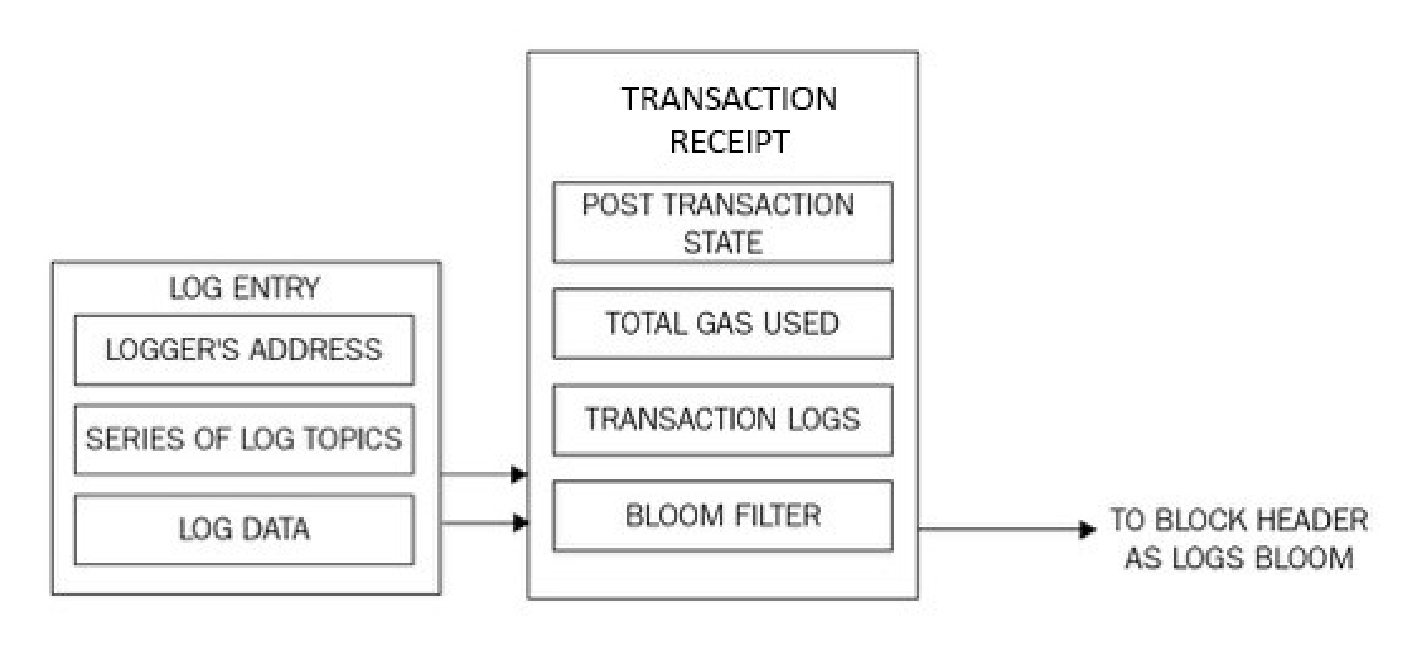
\includegraphics{figuras/ethereum-transaction-receipts.pdf}
\end{frame}

\begin{frame}[allowframebreaks]{The Ethereum Virtual Environment (EVM)}
\protect\hypertarget{the-ethereum-virtual-environment-evm}{}
\begin{itemize}
\tightlist
\item
  Stack size based on LIFO queue: Last In, First Out.
\item
  1024 stack depth limit
\item
  Turing complete but limited by gas, making it quasi-Turing complete
\item
  Big-endian design
\item
  Storage available to EVM

  \begin{itemize}
  \tightlist
  \item
    Memory~
  \item
    Storage
  \item
    Stack
  \end{itemize}
\end{itemize}
\end{frame}

\begin{frame}[allowframebreaks]{EVM operation design}
\protect\hypertarget{evm-operation-design}{}
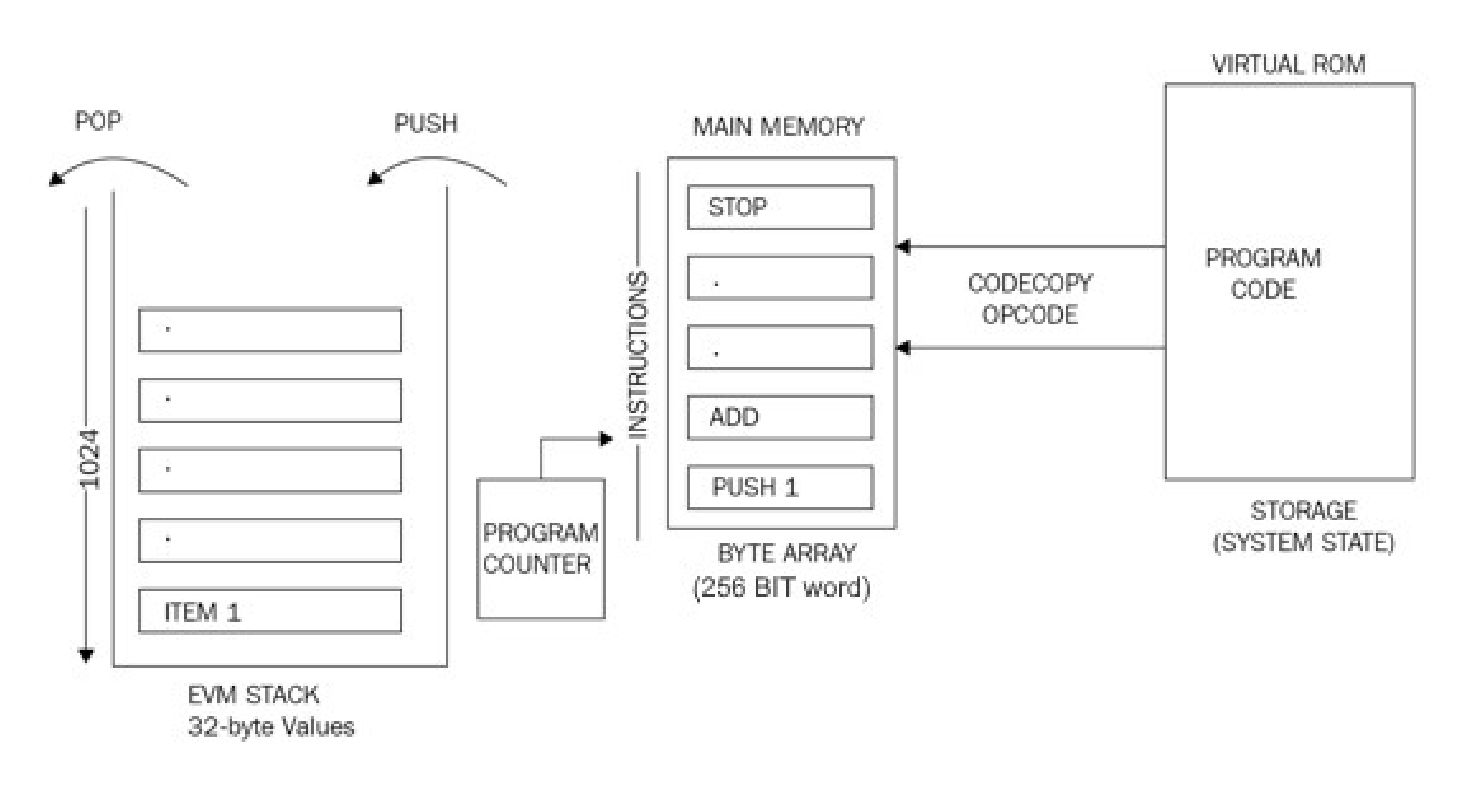
\includegraphics{figuras/ethereum-evm.pdf}
\end{frame}

\begin{frame}[allowframebreaks]{Execution environment}
\protect\hypertarget{execution-environment}{}
\begin{columns}[T]

\column{0.5\textwidth}

O ambiente de execução do \emph{Ethereum} consiste em vários elementos,
como mostrado:

\column{0.5\textwidth}

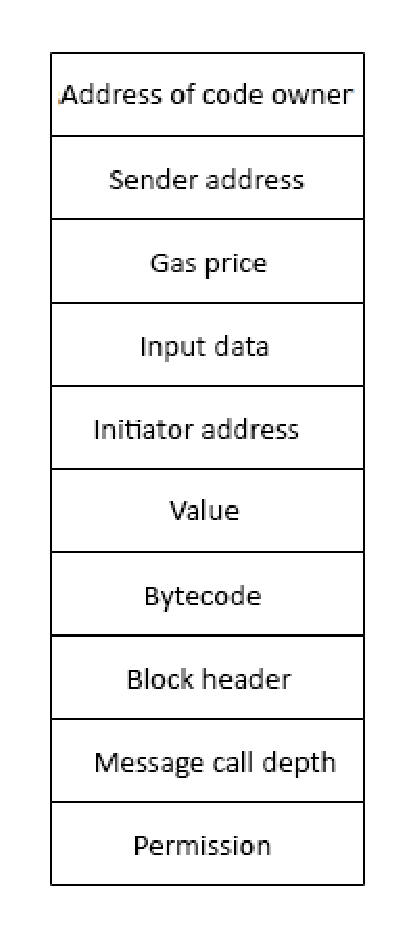
\includegraphics[width=0.5\textwidth,height=\textheight]{figuras/ethereum-execution-env.pdf}

\end{columns}
\end{frame}

\begin{frame}[allowframebreaks]{Machine State}
\protect\hypertarget{machine-state}{}
Uma Máquina de Estado ou \emph{Machine state} é uma tupla compreendendo
vários campos, como mostrado em:

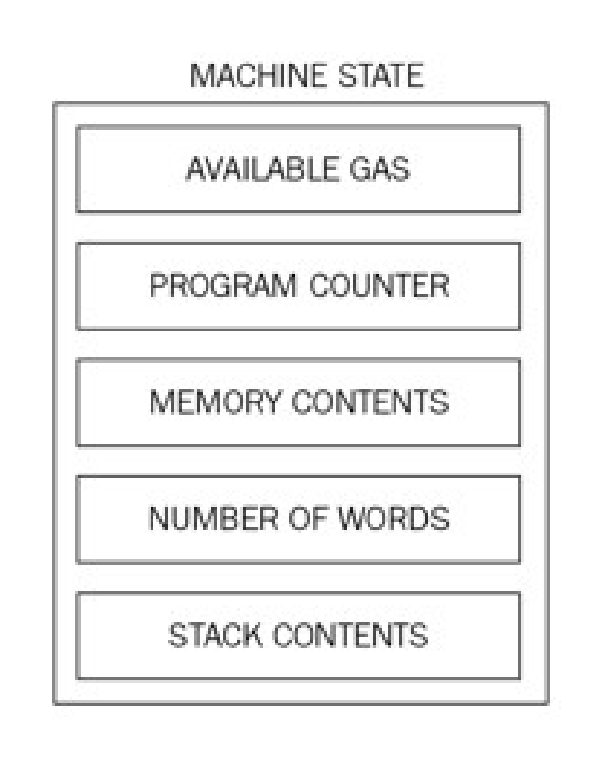
\includegraphics{figuras/ethereum-machine-state.pdf}
\end{frame}

\begin{frame}[allowframebreaks]{Contratos Nativos}
\protect\hypertarget{contratos-nativos}{}
Existem nove contratos pré-compilados ou contratos nativos na versão
Ethereum Istanbul: * \emph{The elliptic curve public key recovery
function} * \emph{The SHA-256-bit hash function}~ * \emph{The
RIPEMD-160-bit hash function}~ * \emph{The identity/datacopy function}~
* \emph{Big mod exponentiation function}~ * \emph{Elliptic curve point
addition function}~ * \emph{Elliptic curve scalar multiplication}~ *
\emph{Elliptic curve pairing}~ * \emph{Blake2 compression function `F'}~
\end{frame}

\hypertarget{um-pouco-mais-de-ethereum}{%
\section{Um pouco mais de Ethereum}\label{um-pouco-mais-de-ethereum}}

\begin{frame}[allowframebreaks]{Outline}
\protect\hypertarget{outline}{}
\begin{itemize}
\tightlist
\item
  Blocos e \emph{Blockchain}
\item
  Wallets e Software Clientes
\item
  Nós e Mineradores
\item
  APIs e ferramentas
\item
  Protocolos suportados
\item
  Linguagens de Programação
\end{itemize}
\end{frame}

\begin{frame}[allowframebreaks]{Blocks e Blockchain}
\protect\hypertarget{blocks-e-blockchain}{}
\begin{columns}[T]

\column{0.5\textwidth}

Um bloco \emph{Ethereum} consiste em vários campos, conforme diagrama.
\emph{State root, transaction root} e \emph{receipts root} são
\emph{root hashes} de suas respectivas árvores.

\column{0.5\textwidth}

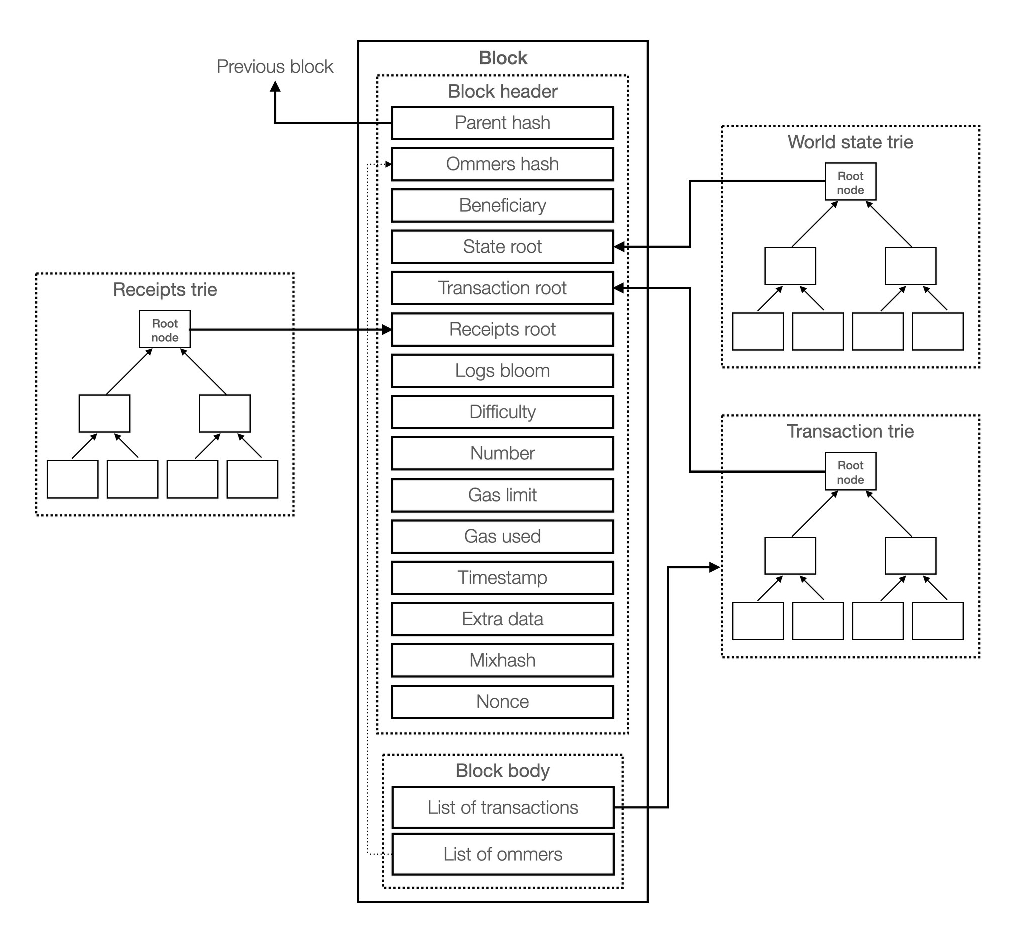
\includegraphics{figuras/ethereum-blocks.pdf}

\end{columns}
\end{frame}

\begin{frame}[allowframebreaks]{Mecanismo de Validação de Blocos}
\protect\hypertarget{mecanismo-de-validauxe7uxe3o-de-blocos}{}
The Ethereum block validation mechanism checks the following conditions:
* If it is consistent with uncles and transactions. This means that all
ommers satisfy the property that they are indeed uncles, and also if the
Proof of Work (PoW) for uncles is valid.~ * If the previous block
(parent) exists and is valid.~ * If the timestamp of the block is valid.
This means that the current block's timestamp must be higher than the
parent block's timestamp. Also, it should be less than 15 minutes into
the future. All block times are calculated in epoch time (Unix time).~

If any of these checks fails, the block will be rejected. A list of
errors for which the block can be rejected is presented here: * The
timestamp is older than the parent~ * There are too many, or duplicate
uncles~\\
* The uncle is an ancestor, or the uncle's parent is not an ancestor *
There is non-positive difficulty~ * There is an invalid mix digest~or
PoW
\end{frame}

\begin{frame}[allowframebreaks]{Finalização de Bloco}
\protect\hypertarget{finalizauxe7uxe3o-de-bloco}{}
Block finalization is a process that is run by miners to validate the
contents of the block and apply rewards. It results in four steps being
executed. These steps are described here:

\begin{enumerate}
\item
  \textbf{Ommers (uncles) validation.} In the case of mining, determine
  ommers. The validation process of the headers of stale blocks checks
  whether the header is valid and whether the relationship between the
  uncle and the current block satisfies the maximum depth of six blocks.
  A block can contain a maximum of two uncles.
\item
  \textbf{Transaction validation.} In the case of mining, determine
  transactions. This process involves checking whether the total gas
  used in the block is equal to the final gas consumption after the
  final transaction, in other words, the cumulative gas used by the
  transactions included in the block.
\item
  \textbf{Reward application.} Apply rewards, which means updating the
  beneficiary's account with a reward balance. In Ethereum, a reward is
  also given to miners for stale blocks, which is 1/32 of the block
  reward. Uncles that are included in the blocks also receive 7/8 of the
  total block reward. The current block reward is 2 ether. It was
  reduced first from 5 ether to 3 with the Byzantium release of
  Ethereum. Later, in the Constantinople release
  (https://blog.ethereum.org/2019/02/22/ethereum-constantinople-st-petersburg-upgrade-announcement/),
  it was reduced further to 2 ether. A block can have a maximum of two
  uncles.
\item
  \textbf{State and nonce validation.} Verify the state and block nonce.
  In the case of mining, compute a valid state and block nonce.
\end{enumerate}
\end{frame}

\begin{frame}[allowframebreaks]{Mecanismo de Block difficulty~}
\protect\hypertarget{mecanismo-de-block-difficulty}{}
O mecanismo de dificuldade do bloco é representado pela fórmula abaixo,
que garante que os blocos sejam produzidos a uma taxa constante:

\(block\_diff = parent\_diff + parent\_diff //' 2048 * max(1 - (block\_timestamp - parent\_timestamp) // 10, -99) + int(2**((block.number // 100000) - 2))\)

O \emph{gas cost} de uma transação pode ser calculado usando esta
fórmula:

\(Total cost = gasUsed * gasPrice\)
\end{frame}

\begin{frame}[fragile,allowframebreaks]{Consumo de Energia}
\protect\hypertarget{consumo-de-energia}{}
\begin{itemize}
\tightlist
\item
  Com a última atualização \texttt{Merge} que trocaram a \emph{Proof of
  Work} (PoW) pela \emph{Proof of Stake} (PoS) tendo como uma das
  motivações a questão ambiental. Houve um grande impacto no consumo de
  energia.
\end{itemize}

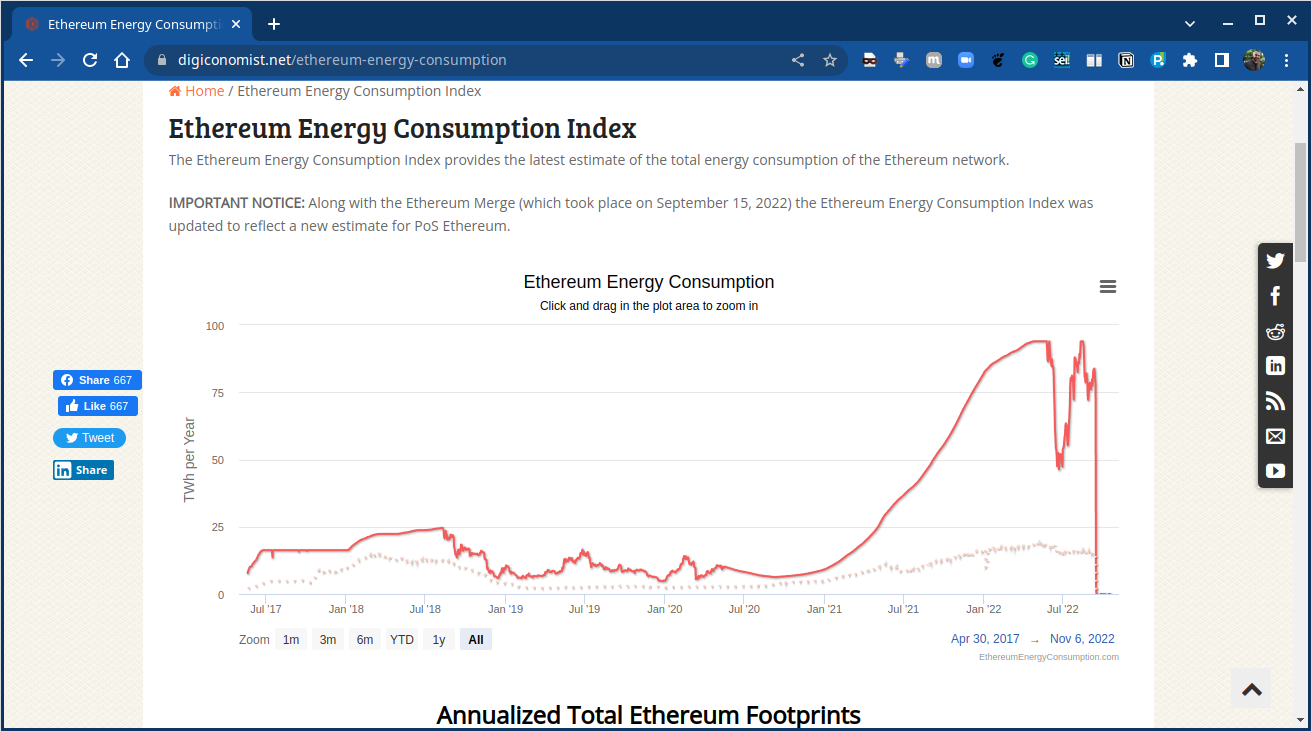
\includegraphics{figuras/ethereum-energy-consumption-page-02.png}
\end{frame}

\begin{frame}[fragile,allowframebreaks]{Wallets e Software Clientes~}
\protect\hypertarget{wallets-e-software-clientes}{}
\begin{itemize}
\tightlist
\item
  Wallets~
\item
  Light clients~
\item
  Existem três tipos de sincronização de clientes:

  \begin{itemize}
  \item
    \textbf{Full:} Nesse modo de sincronização, o cliente \texttt{Geth}
    faz um \emph{download} completo da \emph{blockchain} para o nó
    local. Isso significa que ele obtém todos os cabeçalhos e corpos dos
    blocos e valida todas as transações e blocos desde o bloco
    \emph{genesis}. No início de 2020, o tamanho do \emph{blockchain}
    Ethereum era de aproximadamente \(210GB\), e baixar e manter isso
    pode ser um problema.
  \item
    Hoje, 18 de outubro de 2022 o tamanho chega a \(966.06GB\), segundo
    \url{https://ycharts.com/indicators/ethereum_chain_full_sync_data_size}.
  \item
    \textbf{Fast:} Neste modo é feito o \emph{download} completo, mas
    somente recupera e verifica somente os \(64\) blocos anteriores ao
    bloco corrente. Depois disso, ele verifica os novos blocos na
    íntegra. Não reproduz e verifica todas as transações históricas
    desde o bloco \emph{genesis}, em vez disso, ele só faz os
    \emph{downloads} de estado. Isso também reduz significativamente o
    tamanho do disco do banco de dados \emph{blockchain}. Este é o modo
    padrão de sincronização do cliente \texttt{Geth}.
  \item
    \textbf{Light:} Este é o modo mais rápido e apenas baixa e armazena
    o estado atual. Nesse modo, o cliente não baixa nenhum bloco
    histórico e processa apenas os blocos mais novos.
  \end{itemize}
\end{itemize}
\end{frame}

\begin{frame}[allowframebreaks]{Ethereum keystore: Key decryption
process}
\protect\hypertarget{ethereum-keystore-key-decryption-process}{}
Os arquivos de chave pública e privada são armazenados no diretório
keystore. Os arquivos de keystore Ethereum são arquivos JSON, cujo
conteúdo se parece com o script abaixo.

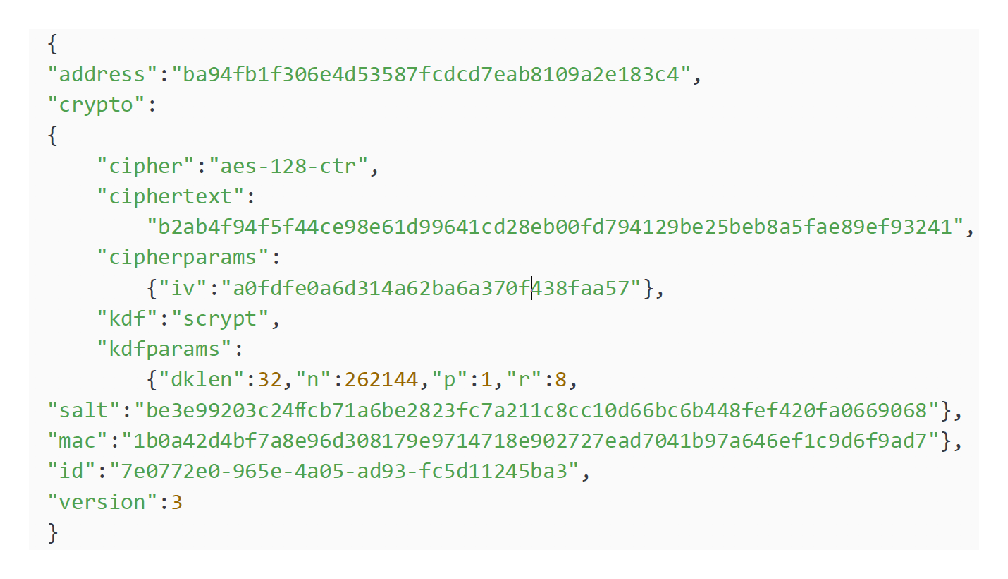
\includegraphics{figuras/ethereum-keys-json.pdf}

\framebreak

Key decryption process:

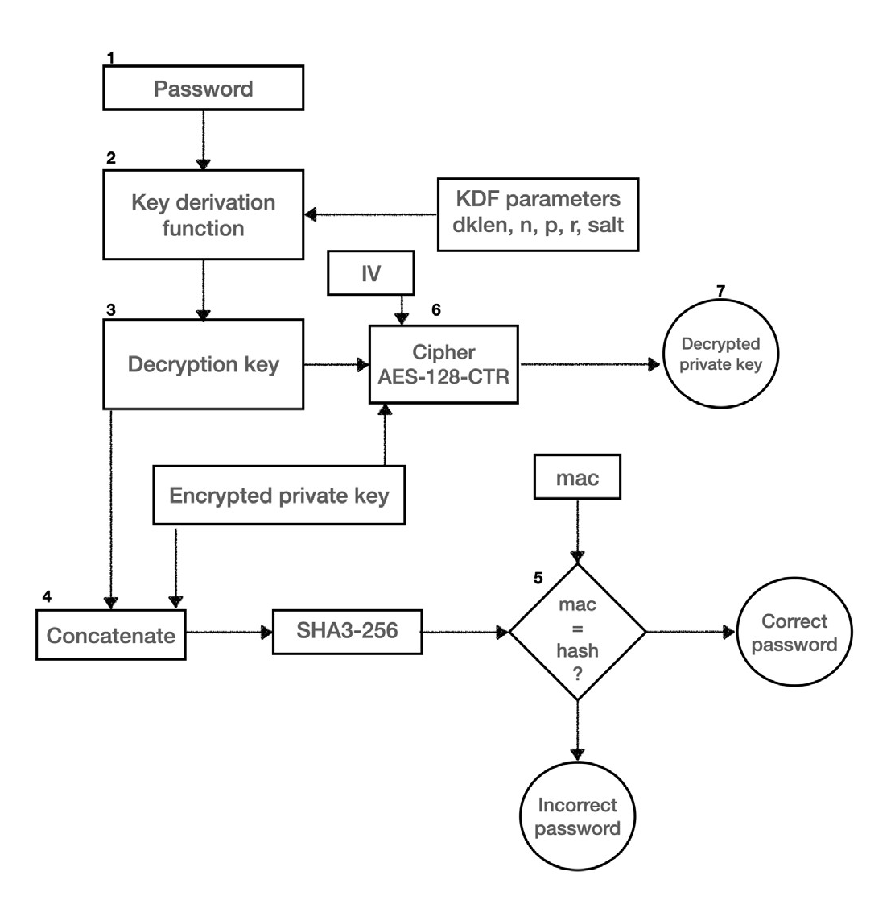
\includegraphics{figuras/ethereum-key-decryption-process.pdf}
\end{frame}

\begin{frame}[fragile,allowframebreaks]{MetaMask}
\protect\hypertarget{metamask}{}
\texttt{MetaMask} é uma carteira de criptomoedas e uma interface para
redes \emph{blockchain} sem exigir a instalação de um nó local.

\begin{columns}[T]

\column{0.5\textwidth}

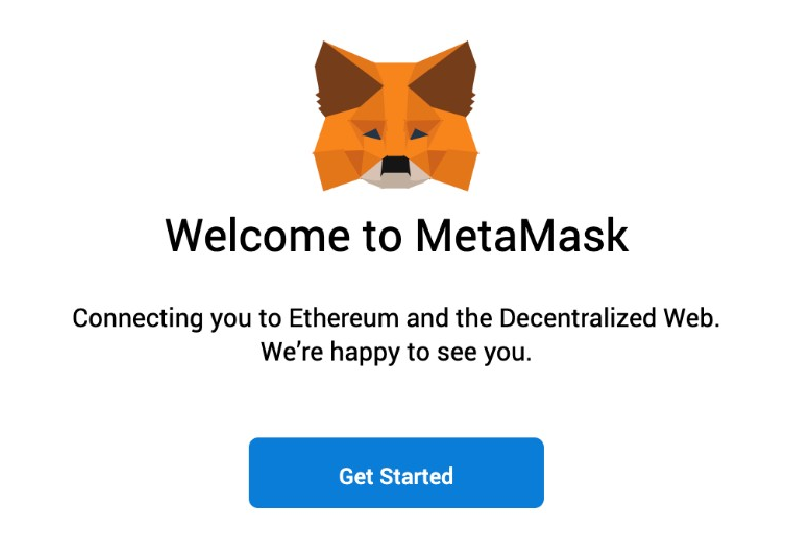
\includegraphics{figuras/metamask-welcome.pdf}

\column{0.5\textwidth}

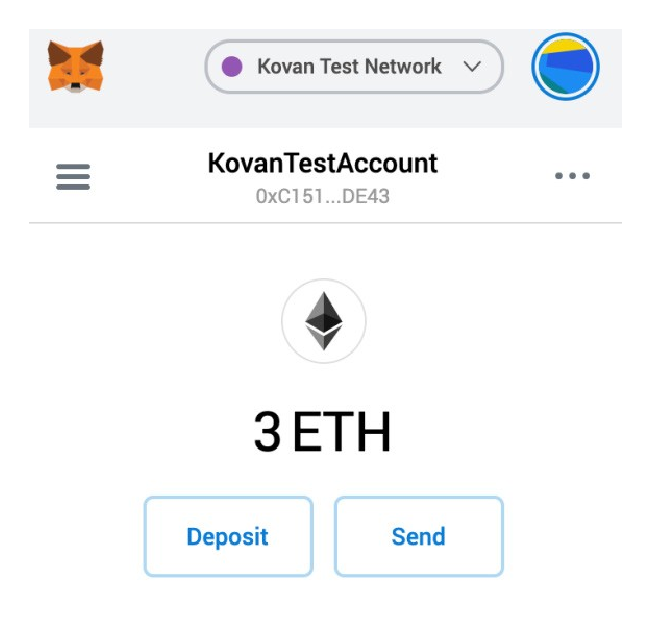
\includegraphics{figuras/metamask-kovantest.pdf}

\end{columns}
\end{frame}

\begin{frame}[allowframebreaks]{Nós e Mineradores~}
\protect\hypertarget{nuxf3s-e-mineradores}{}
A mineração é o processo pelo qual novos blocos são selecionados por
meio de um mecanismo de consenso e adicionados ao \emph{blockchain}. O
processo segue os seguintes passos: * It listens for the transactions
broadcasted on the Ethereum network and determines the transactions to
be processed.~ * It determines stale ommer blocks and includes them in
the blockchain.~ * It updates the account balance with the reward earned
from successfully mining the block. * Finally, a valid state is computed
and the block is finalized, which defines the result of all state
transitions.~
\end{frame}

\begin{frame}[fragile,allowframebreaks]{Ethash}
\protect\hypertarget{ethash}{}
\texttt{Ethash} é o nome do algoritmo de \texttt{Proof\ of\ Work} usado
no \texttt{Ethereum}. 1. First, the header from the previous block and a
32-bit random nonce is combined using Keccak-256.~ 2. This produces a
128-bit structure called \texttt{mix}.~ 3. \texttt{mix} determines which
data is to be picked up from the DAG.~ 4. Once the data is fetched from
the DAG, it is ``mixed'' with the mix to produce the next mix, which is
then again used to fetch data from the DAG and subsequently mixed. This
process is repeated 64 times.~ 5. Eventually, the 64th mix is run
through a digest function to produce a 32-byte sequence.~ 6. This
sequence is compared with the difficulty target. If it is less than the
difficulty target, the nonce is valid, and the PoW is solved. As a
result, the block is mined. If not, then the algorithm repeats with a
new nonce.~
\end{frame}

\begin{frame}[allowframebreaks]{Mineração}
\protect\hypertarget{minerauxe7uxe3o-1}{}
\begin{itemize}
\tightlist
\item
  \textbf{CPU:} Mining using a computer's built in CPU.
\item
  \textbf{GPU:} Mining using graphical processing units, which provide
  better performance as compared to CPUs.
\item
  \textbf{ASICs:} Specialized hardware---Application-Specific Integrated
  Circuit designed solely to run mining algorithms. These are currently
  the most efficient mining tools.
\item
  Mining pools: In mining pools, resources are shared between miners and
  rewards are split accordingly.
\end{itemize}
\end{frame}

\begin{frame}[fragile,allowframebreaks]{Protocolos Suportados}
\protect\hypertarget{protocolos-suportados}{}
Dois principais protocolos de suporte, \texttt{Swarm} e
\texttt{Whisper}, são usados para fornecer armazenamento e mensagens
descentralizadas, a fim de criar um ecossistema descentralizado
completo.

\includegraphics{figuras/ethereum-supporting-protocols.pdf}
\end{frame}

\begin{frame}[allowframebreaks]{Linguagens de Programação}
\protect\hypertarget{linguagens-de-programauxe7uxe3o}{}
\begin{itemize}
\tightlist
\item
  \textbf{Solidity} is one of the high-level languages that has been
  developed for Ethereum. It uses JavaScript-like syntax to write code
  for smart contracts. Once the code is written, it is compiled into
  bytecode that's understandable by the EVM using the Solidity compiler
  called solc.~
\item
  \textbf{LLL} is another language that is used to write smart contract
  code.~
\item
  \textbf{Serpent} is a Python-like, high-level language that can be
  used to write smart contracts for Ethereum.~
\item
  \textbf{Vyper} is a newer language that has been developed from
  scratch to achieve a secure, simple, and auditable language.
\end{itemize}
\end{frame}

\begin{frame}[fragile]{Atividade}
\protect\hypertarget{atividade-2}{}
\begin{itemize}
\tightlist
\item
  Leitura do \texttt{Ethereum\ yellow\ paper}:
  \url{https://ethereum.github.io/yellowpaper/paper.pdf}
\item
  Instalação do \texttt{Geth} e executar ele com a
  \texttt{Kovan\ testnet}.
\end{itemize}
\end{frame}

\begin{frame}{Leitura Recomendada}
\protect\hypertarget{leitura-recomendada-2}{}
\normalsize

\begin{alertblock}{Leitura Recomendada}

\textbf{Capítulo 11: Ethereum 101}

\textbf{Livro}:
\href{https://search.ebscohost.com/login.aspx?direct=true\&db=e000xww\&AN=1789486\&authtype=shib\&lang=pt-br\&site=eds-live\&scope=site\&ebv=EB\&ppid=pp_276}{IMRAN
BASHIR. Mastering Blockchain\,: Distributed Ledger Technology,
Decentralization, and Smart Contracts Explained, 2nd Edition.}

\textbf{Capítulo 12: Futher Ethereum}

\textbf{Livro}:
\href{https://search.ebscohost.com/login.aspx?direct=true\&db=e000xww\&AN=1789486\&authtype=shib\&lang=pt-br\&site=eds-live\&scope=site\&ebv=EB\&ppid=pp_310}{IMRAN
BASHIR. Mastering Blockchain\,: Distributed Ledger Technology,
Decentralization, and Smart Contracts Explained, 2nd Edition.}

\end{alertblock}
\end{frame}

\hypertarget{pruxe1tica-sobre-ethereum}{%
\section{Prática sobre Ethereum}\label{pruxe1tica-sobre-ethereum}}

\hypertarget{leitura-do-capuxedtulo-12-futher-ethereum}{%
\section{\texorpdfstring{Leitura do Capítulo 12: \emph{Futher
Ethereum}}{Leitura do Capítulo 12: Futher Ethereum}}\label{leitura-do-capuxedtulo-12-futher-ethereum}}

\begin{frame}[fragile]{Leitura do Capítulo 12: \emph{Futher Ethereum}}
\begin{enumerate}
\item
  Faça a leitura do
  \href{https://search.ebscohost.com/login.aspx?direct=true\&db=e000xww\&AN=1789486\&authtype=shib\&lang=pt-br\&site=eds-live\&scope=site\&ebv=EB\&ppid=pp_310}{Capítulo
  12: \emph{Futher Ethereum}}
\item
  Instalar as ferramentas e testar os comandos apresentados no capítulo.
\end{enumerate}

O cliente padrão \texttt{Geth} pode ser instalado em sistema derivados
do Ubuntu:

\begin{Shaded}
\begin{Highlighting}[]
\ExtensionTok{$}\NormalTok{ sudo apt{-}get install }\AttributeTok{{-}y}\NormalTok{ software{-}properties{-}common}
\ExtensionTok{$}\NormalTok{ sudo add{-}apt{-}repository }\AttributeTok{{-}y}\NormalTok{ ppa:ethereum/ethereum}
\ExtensionTok{$}\NormalTok{ sudo apt{-}get update}
\ExtensionTok{$}\NormalTok{ sudo apt{-}get install }\AttributeTok{{-}y}\NormalTok{ ethereum}
\end{Highlighting}
\end{Shaded}

Em outros Sistemas como o \texttt{Manjaro}:

\begin{Shaded}
\begin{Highlighting}[]
\ExtensionTok{[rag@nitro{-}ryzen}\NormalTok{ \textasciitilde{}]$ sudo pacaur }\AttributeTok{{-}Ss}\NormalTok{ ethereum}
\ExtensionTok{community/go{-}ethereum}\NormalTok{ 1.10.25{-}1 }\PreprocessorTok{[}\SpecialStringTok{instalado}\PreprocessorTok{]}
    \ExtensionTok{Official}\NormalTok{ Go implementation of the Ethereum protocol}
\ExtensionTok{[rag@nitro{-}ryzen}\NormalTok{ \textasciitilde{}]$ sudo pacaur }\AttributeTok{{-}S}\NormalTok{ go{-}ethereum}
\ExtensionTok{[rag@nitro{-}ryzen}\NormalTok{ \textasciitilde{}]$ pacaur }\AttributeTok{{-}S}\NormalTok{ go{-}ethereum}
\ExtensionTok{resolvendo}\NormalTok{ dependencias...}
\ExtensionTok{procurando}\NormalTok{ pacotes conflitantes...}

\ExtensionTok{Pacotes} \ErrorTok{(}\ExtensionTok{1}\KeywordTok{)} \ExtensionTok{go{-}ethereum{-}1.10.25{-}1}

\ExtensionTok{Tamanho}\NormalTok{ total instalado:  197,38 MiB}
\ExtensionTok{Alteração}\NormalTok{ no tamanho:       0,00 MiB}

\ExtensionTok{::}\NormalTok{ Continuar a instalação}\PreprocessorTok{?} \PreprocessorTok{[}\SpecialStringTok{S/n}\PreprocessorTok{]}
\end{Highlighting}
\end{Shaded}

Instruções para outros Sistemas Operacionais podem ser encontradas no
site oficial da documentação do \texttt{Ethereum}
\url{https://geth.ethereum.org/docs/install-and-build/installing-geth}.

Executando o \texttt{Geth} diretamente ele irá sincronizar com a rede
principal do \texttt{Ethereum}, a \texttt{mainnet}.

\begin{Shaded}
\begin{Highlighting}[]
\ExtensionTok{[rag@nitro{-}ryzen}\NormalTok{ \textasciitilde{}]$ geth}
\ExtensionTok{INFO}\NormalTok{ [10{-}20}\KeywordTok{|}\ExtensionTok{21:07:12.911]}\NormalTok{ Starting Geth on Ethereum mainnet... }
\ExtensionTok{INFO}\NormalTok{ [10{-}20}\KeywordTok{|}\ExtensionTok{21:07:12.912]}\NormalTok{ Bumping default cache on mainnet         provided=1024 updated=4096}
\ExtensionTok{INFO}\NormalTok{ [10{-}20}\KeywordTok{|}\ExtensionTok{21:07:12.914]}\NormalTok{ Maximum peer count                       ETH=50 LES=0 total=50}
\ExtensionTok{INFO}\NormalTok{ [10{-}20}\KeywordTok{|}\ExtensionTok{21:07:12.915]}\NormalTok{ Smartcard socket not found, disabling    err=}\StringTok{"stat /run/pcscd/pcscd.comm: no such file or directory"}
\ExtensionTok{INFO}\NormalTok{ [10{-}20}\KeywordTok{|}\ExtensionTok{21:07:12.920]}\NormalTok{ Set global gas cap                       cap=50,000,000}
\ExtensionTok{INFO}\NormalTok{ [10{-}20}\KeywordTok{|}\ExtensionTok{21:07:12.922]}\NormalTok{ Allocated trie memory caches             clean=614.00MiB dirty=1024.00MiB}
\ExtensionTok{INFO}\NormalTok{ [10{-}20}\KeywordTok{|}\ExtensionTok{21:07:12.923]}\NormalTok{ Allocated cache and file handles         database=/home/rag/.ethereum/geth/chaindata cache=2.00GiB handles=262,144}
\ExtensionTok{INFO}\NormalTok{ [10{-}20}\KeywordTok{|}\ExtensionTok{21:07:12.946]}\NormalTok{ Opened ancient database                  database=/home/rag/.ethereum/geth/chaindata/ancient/chain readonly=false}
\ExtensionTok{INFO}\NormalTok{ [10{-}20}\KeywordTok{|}\ExtensionTok{21:07:12.950]}  
\ExtensionTok{INFO}\NormalTok{ [10{-}20}\KeywordTok{|}\ExtensionTok{21:07:12.950]} \AttributeTok{{-}{-}{-}{-}{-}{-}{-}{-}{-}{-}{-}{-}{-}{-}{-}{-}{-}{-}{-}{-}{-}{-}{-}{-}{-}{-}{-}{-}{-}{-}{-}{-}{-}{-}{-}{-}{-}{-}{-}{-}{-}{-}{-}{-}{-}{-}{-}{-}{-}{-}{-}{-}{-}{-}{-}{-}{-}{-}{-}{-}{-}{-}{-}{-}{-}{-}{-}{-}{-}{-}{-}{-}{-}{-}{-}{-}{-}{-}{-}{-}{-}{-}{-}}
\ExtensionTok{INFO}\NormalTok{ [10{-}20}\KeywordTok{|}\ExtensionTok{21:07:12.950]}\NormalTok{ Chain ID:  1 }\ErrorTok{(}\ExtensionTok{mainnet}\KeywordTok{)} 
\ExtensionTok{INFO}\NormalTok{ [10{-}20}\KeywordTok{|}\ExtensionTok{21:07:12.950]}\NormalTok{ Consensus: Beacon }\ErrorTok{(}\ExtensionTok{proof{-}of{-}stake}\KeywordTok{)}\ExtensionTok{,}\NormalTok{ merged from Ethash }\ErrorTok{(}\ExtensionTok{proof{-}of{-}work}\KeywordTok{)} 
\ExtensionTok{INFO}\NormalTok{ [10{-}20}\KeywordTok{|}\ExtensionTok{21:07:12.950]}  
\ExtensionTok{INFO}\NormalTok{ [10{-}20}\KeywordTok{|}\ExtensionTok{21:07:12.950]}\NormalTok{ Pre{-}Merge hard forks: }
\ExtensionTok{INFO}\NormalTok{ [10{-}20}\KeywordTok{|}\ExtensionTok{21:07:12.950]}  \AttributeTok{{-}}\NormalTok{ Homestead:                   1150000  }\ErrorTok{(}\ExtensionTok{https://github.com/ethereum/execution{-}specs/blob/master/network{-}upgrades/mainnet{-}upgrades/homestead.md}\KeywordTok{)} 
\ExtensionTok{INFO}\NormalTok{ [10{-}20}\KeywordTok{|}\ExtensionTok{21:07:12.950]}  \AttributeTok{{-}}\NormalTok{ DAO Fork:                    1920000  }\ErrorTok{(}\ExtensionTok{https://github.com/ethereum/execution{-}specs/blob/master/network{-}upgrades/mainnet{-}upgrades/dao{-}fork.md}\KeywordTok{)} 
\ExtensionTok{INFO}\NormalTok{ [10{-}20}\KeywordTok{|}\ExtensionTok{21:07:12.950]}  \AttributeTok{{-}}\NormalTok{ Tangerine Whistle }\ErrorTok{(}\ExtensionTok{EIP}\NormalTok{ 150}\KeywordTok{)}\BuiltInTok{:}\NormalTok{ 2463000  }\ErrorTok{(}\ExtensionTok{https://github.com/ethereum/execution{-}specs/blob/master/network{-}upgrades/mainnet{-}upgrades/tangerine{-}whistle.md}\KeywordTok{)} 
\ExtensionTok{INFO}\NormalTok{ [10{-}20}\KeywordTok{|}\ExtensionTok{21:07:12.950]}  \AttributeTok{{-}}\NormalTok{ Spurious Dragon/1 }\ErrorTok{(}\ExtensionTok{EIP}\NormalTok{ 155}\KeywordTok{)}\BuiltInTok{:}\NormalTok{ 2675000  }\ErrorTok{(}\ExtensionTok{https://github.com/ethereum/execution{-}specs/blob/master/network{-}upgrades/mainnet{-}upgrades/spurious{-}dragon.md}\KeywordTok{)} 
\ExtensionTok{INFO}\NormalTok{ [10{-}20}\KeywordTok{|}\ExtensionTok{21:07:12.950]}  \AttributeTok{{-}}\NormalTok{ Spurious Dragon/2 }\ErrorTok{(}\ExtensionTok{EIP}\NormalTok{ 158}\KeywordTok{)}\BuiltInTok{:}\NormalTok{ 2675000  }\ErrorTok{(}\ExtensionTok{https://github.com/ethereum/execution{-}specs/blob/master/network{-}upgrades/mainnet{-}upgrades/spurious{-}dragon.md}\KeywordTok{)} 
\ExtensionTok{INFO}\NormalTok{ [10{-}20}\KeywordTok{|}\ExtensionTok{21:07:12.950]}  \AttributeTok{{-}}\NormalTok{ Byzantium:                   4370000  }\ErrorTok{(}\ExtensionTok{https://github.com/ethereum/execution{-}specs/blob/master/network{-}upgrades/mainnet{-}upgrades/byzantium.md}\KeywordTok{)} 
\ExtensionTok{INFO}\NormalTok{ [10{-}20}\KeywordTok{|}\ExtensionTok{21:07:12.950]}  \AttributeTok{{-}}\NormalTok{ Constantinople:              7280000  }\ErrorTok{(}\ExtensionTok{https://github.com/ethereum/execution{-}specs/blob/master/network{-}upgrades/mainnet{-}upgrades/constantinople.md}\KeywordTok{)} 
\ExtensionTok{INFO}\NormalTok{ [10{-}20}\KeywordTok{|}\ExtensionTok{21:07:12.950]}  \AttributeTok{{-}}\NormalTok{ Petersburg:                  7280000  }\ErrorTok{(}\ExtensionTok{https://github.com/ethereum/execution{-}specs/blob/master/network{-}upgrades/mainnet{-}upgrades/petersburg.md}\KeywordTok{)} 
\ExtensionTok{INFO}\NormalTok{ [10{-}20}\KeywordTok{|}\ExtensionTok{21:07:12.950]}  \AttributeTok{{-}}\NormalTok{ Istanbul:                    9069000  }\ErrorTok{(}\ExtensionTok{https://github.com/ethereum/execution{-}specs/blob/master/network{-}upgrades/mainnet{-}upgrades/istanbul.md}\KeywordTok{)} 
\ExtensionTok{INFO}\NormalTok{ [10{-}20}\KeywordTok{|}\ExtensionTok{21:07:12.950]}  \AttributeTok{{-}}\NormalTok{ Muir Glacier:                9200000  }\ErrorTok{(}\ExtensionTok{https://github.com/ethereum/execution{-}specs/blob/master/network{-}upgrades/mainnet{-}upgrades/muir{-}glacier.md}\KeywordTok{)} 
\ExtensionTok{INFO}\NormalTok{ [10{-}20}\KeywordTok{|}\ExtensionTok{21:07:12.950]}  \AttributeTok{{-}}\NormalTok{ Berlin:                      12244000 }\ErrorTok{(}\ExtensionTok{https://github.com/ethereum/execution{-}specs/blob/master/network{-}upgrades/mainnet{-}upgrades/berlin.md}\KeywordTok{)} 
\ExtensionTok{INFO}\NormalTok{ [10{-}20}\KeywordTok{|}\ExtensionTok{21:07:12.950]}  \AttributeTok{{-}}\NormalTok{ London:                      12965000 }\ErrorTok{(}\ExtensionTok{https://github.com/ethereum/execution{-}specs/blob/master/network{-}upgrades/mainnet{-}upgrades/london.md}\KeywordTok{)} 
\ExtensionTok{INFO}\NormalTok{ [10{-}20}\KeywordTok{|}\ExtensionTok{21:07:12.950]}  \AttributeTok{{-}}\NormalTok{ Arrow Glacier:               13773000 }\ErrorTok{(}\ExtensionTok{https://github.com/ethereum/execution{-}specs/blob/master/network{-}upgrades/mainnet{-}upgrades/arrow{-}glacier.md}\KeywordTok{)} 
\ExtensionTok{INFO}\NormalTok{ [10{-}20}\KeywordTok{|}\ExtensionTok{21:07:12.950]}  \AttributeTok{{-}}\NormalTok{ Gray Glacier:                15050000 }\ErrorTok{(}\ExtensionTok{https://github.com/ethereum/execution{-}specs/blob/master/network{-}upgrades/mainnet{-}upgrades/gray{-}glacier.md}\KeywordTok{)} 
\ExtensionTok{INFO}\NormalTok{ [10{-}20}\KeywordTok{|}\ExtensionTok{21:07:12.950]}  
\ExtensionTok{INFO}\NormalTok{ [10{-}20}\KeywordTok{|}\ExtensionTok{21:07:12.950]}\NormalTok{ Merge configured: }
\ExtensionTok{INFO}\NormalTok{ [10{-}20}\KeywordTok{|}\ExtensionTok{21:07:12.950]}  \AttributeTok{{-}}\NormalTok{ Hard{-}fork specification:    https://github.com/ethereum/execution{-}specs/blob/master/network{-}upgrades/mainnet{-}upgrades/paris.md }
\ExtensionTok{INFO}\NormalTok{ [10{-}20}\KeywordTok{|}\ExtensionTok{21:07:12.950]}  \AttributeTok{{-}}\NormalTok{ Network known to be merged: true }
\ExtensionTok{INFO}\NormalTok{ [10{-}20}\KeywordTok{|}\ExtensionTok{21:07:12.950]}  \AttributeTok{{-}}\NormalTok{ Total terminal difficulty:  58750000000000000000000 }
\ExtensionTok{INFO}\NormalTok{ [10{-}20}\KeywordTok{|}\ExtensionTok{21:07:12.950]}  \AttributeTok{{-}}\NormalTok{ Merge netsplit block:       }\OperatorTok{\textless{}}\NormalTok{nil}\OperatorTok{\textgreater{}} 
\ExtensionTok{INFO}\NormalTok{ [10{-}20}\KeywordTok{|}\ExtensionTok{21:07:12.950]} \AttributeTok{{-}{-}{-}{-}{-}{-}{-}{-}{-}{-}{-}{-}{-}{-}{-}{-}{-}{-}{-}{-}{-}{-}{-}{-}{-}{-}{-}{-}{-}{-}{-}{-}{-}{-}{-}{-}{-}{-}{-}{-}{-}{-}{-}{-}{-}{-}{-}{-}{-}{-}{-}{-}{-}{-}{-}{-}{-}{-}{-}{-}{-}{-}{-}{-}{-}{-}{-}{-}{-}{-}{-}{-}{-}{-}{-}{-}{-}{-}{-}{-}{-}{-}{-}{-}{-}{-}}
\ExtensionTok{INFO}\NormalTok{ [10{-}20}\KeywordTok{|}\ExtensionTok{21:07:12.950]}  
\ExtensionTok{INFO}\NormalTok{ [10{-}20}\KeywordTok{|}\ExtensionTok{21:07:12.952]}\NormalTok{ Disk storage enabled for ethash caches   dir=/home/rag/.ethereum/geth/ethash count=3}
\ExtensionTok{INFO}\NormalTok{ [10{-}20}\KeywordTok{|}\ExtensionTok{21:07:12.952]}\NormalTok{ Disk storage enabled for ethash DAGs     dir=/home/rag/.ethash               count=2}
\ExtensionTok{INFO}\NormalTok{ [10{-}20}\KeywordTok{|}\ExtensionTok{21:07:12.952]}\NormalTok{ Initialising Ethereum protocol           network=1 dbversion=8}
\ExtensionTok{INFO}\NormalTok{ [10{-}20}\KeywordTok{|}\ExtensionTok{21:07:12.963]}\NormalTok{ Loaded most recent local header          number=0 hash=d4e567..cb8fa3 td=17,179,869,184 age=53y6mo3w}
\ExtensionTok{INFO}\NormalTok{ [10{-}20}\KeywordTok{|}\ExtensionTok{21:07:12.963]}\NormalTok{ Loaded most recent local full block      number=0 hash=d4e567..cb8fa3 td=17,179,869,184 age=53y6mo3w}
\ExtensionTok{INFO}\NormalTok{ [10{-}20}\KeywordTok{|}\ExtensionTok{21:07:12.963]}\NormalTok{ Loaded most recent local fast block      number=0 hash=d4e567..cb8fa3 td=17,179,869,184 age=53y6mo3w}
\ExtensionTok{INFO}\NormalTok{ [10{-}20}\KeywordTok{|}\ExtensionTok{21:07:12.964]}\NormalTok{ Loaded local transaction journal         transactions=0 dropped=0}
\ExtensionTok{INFO}\NormalTok{ [10{-}20}\KeywordTok{|}\ExtensionTok{21:07:12.964]}\NormalTok{ Regenerated local transaction journal    transactions=0 accounts=0}
\ExtensionTok{INFO}\NormalTok{ [10{-}20}\KeywordTok{|}\ExtensionTok{21:07:12.965]}\NormalTok{ Chain post{-}merge, sync via beacon client }
\ExtensionTok{INFO}\NormalTok{ [10{-}20}\KeywordTok{|}\ExtensionTok{21:07:12.965]}\NormalTok{ Gasprice oracle is ignoring threshold set threshold=2}
\ExtensionTok{WARN}\NormalTok{ [10{-}20}\KeywordTok{|}\ExtensionTok{21:07:12.965]}\NormalTok{ Engine API enabled                       protocol=eth}
\ExtensionTok{INFO}\NormalTok{ [10{-}20}\KeywordTok{|}\ExtensionTok{21:07:12.966]}\NormalTok{ Starting peer{-}to{-}peer node               instance=Geth/v1.10.25{-}stable{-}69568c55/linux{-}amd64/go1.19.1}
\ExtensionTok{INFO}\NormalTok{ [10{-}20}\KeywordTok{|}\ExtensionTok{21:07:12.991]}\NormalTok{ New local node record                    seq=1,665,519,113,919 id=da440578e33a2ce7 ip=127.0.0.1 udp=30303 tcp=30303}
\ExtensionTok{INFO}\NormalTok{ [10{-}20}\KeywordTok{|}\ExtensionTok{21:07:12.992]}\NormalTok{ Started P2P networking                   self=enode://9ae8fcdad4a7243d1bd2308a159c5800ec170e588862be110152627c9ed3fa67376ef8c7526d7a56e9bb72da729cf792c7bef86c095471995cc352f9e353acfc@127.0.0.1:30303}
\ExtensionTok{INFO}\NormalTok{ [10{-}20}\KeywordTok{|}\ExtensionTok{21:07:12.993]}\NormalTok{ IPC endpoint opened                      url=/home/rag/.ethereum/geth.ipc}
\ExtensionTok{INFO}\NormalTok{ [10{-}20}\KeywordTok{|}\ExtensionTok{21:07:12.993]}\NormalTok{ Loaded JWT secret file                   path=/home/rag/.ethereum/geth/jwtsecret crc32=0xdeccafe4}
\ExtensionTok{INFO}\NormalTok{ [10{-}20}\KeywordTok{|}\ExtensionTok{21:07:12.994]}\NormalTok{ WebSocket enabled                        url=ws://127.0.0.1:8551}
\ExtensionTok{INFO}\NormalTok{ [10{-}20}\KeywordTok{|}\ExtensionTok{21:07:12.994]}\NormalTok{ HTTP server started                      endpoint=127.0.0.1:8551 auth=true prefix= cors=localhost vhosts=localhost}
\ExtensionTok{INFO}\NormalTok{ [10{-}20}\KeywordTok{|}\ExtensionTok{21:07:16.251]}\NormalTok{ New local node record                    seq=1,665,519,113,920 id=da440578e33a2ce7 ip=187.95.110.26 udp=2770  tcp=30303}
\ExtensionTok{INFO}\NormalTok{ [10{-}20}\KeywordTok{|}\ExtensionTok{21:07:22.992]}\NormalTok{ Looking for peers                        peercount=0 tried=2 static=0}
\ExtensionTok{INFO}\NormalTok{ [10{-}20}\KeywordTok{|}\ExtensionTok{21:07:32.994]}\NormalTok{ Looking for peers                        peercount=0 tried=3 static=0}
\ExtensionTok{INFO}\NormalTok{ [10{-}20}\KeywordTok{|}\ExtensionTok{21:07:43.205]}\NormalTok{ Looking for peers                        peercount=0 tried=9 static=0}
\ExtensionTok{WARN}\NormalTok{ [10{-}20}\KeywordTok{|}\ExtensionTok{21:07:47.967]}\NormalTok{ Post{-}merge network, but no beacon client seen. Please launch one to follow the chain! }
\ExtensionTok{INFO}\NormalTok{ [10{-}20}\KeywordTok{|}\ExtensionTok{21:07:53.281]}\NormalTok{ Looking for peers                        peercount=0 tried=13 static=0}
\ExtensionTok{INFO}\NormalTok{ [10{-}20}\KeywordTok{|}\ExtensionTok{21:08:03.346]}\NormalTok{ Looking for peers                        peercount=0 tried=9  static=0}
\end{Highlighting}
\end{Shaded}

Criando uma nova conta:

\begin{Shaded}
\begin{Highlighting}[]
\ExtensionTok{[rag@nitro{-}ryzen}\NormalTok{ \textasciitilde{}]$ geth account new}
\ExtensionTok{INFO}\NormalTok{ [10{-}20}\KeywordTok{|}\ExtensionTok{21:13:44.948]}\NormalTok{ Maximum peer count                       ETH=50 LES=0 total=50}
\ExtensionTok{INFO}\NormalTok{ [10{-}20}\KeywordTok{|}\ExtensionTok{21:13:44.949]}\NormalTok{ Smartcard socket not found, disabling    err=}\StringTok{"stat /run/pcscd/pcscd.comm: no such file or directory"}
\ExtensionTok{Your}\NormalTok{ new account is locked with a password. Please give a password. Do not forget this password.}
\ExtensionTok{Password:} 
\ExtensionTok{Repeat}\NormalTok{ password: }

\ExtensionTok{Your}\NormalTok{ new key was generated}

\ExtensionTok{Public}\NormalTok{ address of the key:   0x668a07cAf4f4b2A5939051d25DA2334a4c425599}
\ExtensionTok{Path}\NormalTok{ of the secret key file: /home/rag/.ethereum/keystore/UTC{-}{-}2022{-}10{-}21T00{-}14{-}13.552574058Z{-}{-}668a07caf4f4b2a5939051d25da2334a4c425599}

\ExtensionTok{{-}}\NormalTok{ You can share your public address with anyone. Others need it to interact with you.}
\ExtensionTok{{-}}\NormalTok{ You must NEVER share the secret key with anyone! The key controls access to your funds!}
\ExtensionTok{{-}}\NormalTok{ You must BACKUP your key file! Without the key, it}\StringTok{\textquotesingle{}s impossible to access account funds!}
\StringTok{{-} You must REMEMBER your password! Without the password, it\textquotesingle{}}\NormalTok{s impossible to decrypt the key!}

\ExtensionTok{[rag@nitro{-}ryzen}\NormalTok{ \textasciitilde{}]$ }
\end{Highlighting}
\end{Shaded}

As contas existentes ou que foram criadas podem ser listadas com o
comando:

\begin{Shaded}
\begin{Highlighting}[]
\ExtensionTok{[rag@nitro{-}ryzen}\NormalTok{ \textasciitilde{}]$ geth account list}
\ExtensionTok{INFO}\NormalTok{ [10{-}20}\KeywordTok{|}\ExtensionTok{21:15:41.981]}\NormalTok{ Maximum peer count                       ETH=50 LES=0 total=50}
\ExtensionTok{INFO}\NormalTok{ [10{-}20}\KeywordTok{|}\ExtensionTok{21:15:41.982]}\NormalTok{ Smartcard socket not found, disabling    err=}\StringTok{"stat /run/pcscd/pcscd.comm: no such file or directory"}
\ExtensionTok{INFO}\NormalTok{ [10{-}20}\KeywordTok{|}\ExtensionTok{21:15:41.982]}\NormalTok{ Set global gas cap                       cap=50,000,000}
\ExtensionTok{Account} \CommentTok{\#0: \{668a07caf4f4b2a5939051d25da2334a4c425599\} keystore:///home/rag/.ethereum/keystore/UTC{-}{-}2022{-}10{-}21T00{-}14{-}13.552574058Z{-}{-}668a07caf4f4b2a5939051d25da2334a4c425599}
\ExtensionTok{[rag@nitro{-}ryzen}\NormalTok{ \textasciitilde{}]$}
\end{Highlighting}
\end{Shaded}

A documentação, bem como comandos e parâmetros podem ser acessados em
\url{https://geth.ethereum.org/docs}

Executando com opção de responder a comandos via \texttt{RPC}. A
documentação desta parte está disponível em
\url{https://geth.ethereum.org/docs/rpc/server}.

\begin{Shaded}
\begin{Highlighting}[]
\ExtensionTok{[rag@nitro{-}ryzen}\NormalTok{ \textasciitilde{}]$ geth }\AttributeTok{{-}{-}mainnet} \AttributeTok{{-}{-}syncmode}\NormalTok{ snap }\AttributeTok{{-}{-}http} \AttributeTok{{-}{-}http.addr}\NormalTok{ 127.0.0.1 }\AttributeTok{{-}{-}http.port}\NormalTok{ 8559 }\AttributeTok{{-}{-}http.api} \StringTok{"eth,net,web3,personal"}
\ExtensionTok{INFO}\NormalTok{ [10{-}20}\KeywordTok{|}\ExtensionTok{21:57:05.774]}\NormalTok{ Starting Geth on Ethereum mainnet... }
\ExtensionTok{INFO}\NormalTok{ [10{-}20}\KeywordTok{|}\ExtensionTok{21:57:05.775]}\NormalTok{ Bumping default cache on mainnet         provided=1024 updated=4096}
\ExtensionTok{INFO}\NormalTok{ [10{-}20}\KeywordTok{|}\ExtensionTok{21:57:05.777]}\NormalTok{ Maximum peer count                       ETH=50 LES=0 total=50}
\ExtensionTok{INFO}\NormalTok{ [10{-}20}\KeywordTok{|}\ExtensionTok{21:57:05.779]}\NormalTok{ Smartcard socket not found, disabling    err=}\StringTok{"stat /run/pcscd/pcscd.comm: no such file or directory"}
\ExtensionTok{INFO}\NormalTok{ [10{-}20}\KeywordTok{|}\ExtensionTok{21:57:05.784]}\NormalTok{ Set global gas cap                       cap=50,000,000}
\ExtensionTok{INFO}\NormalTok{ [10{-}20}\KeywordTok{|}\ExtensionTok{21:57:05.815]}\NormalTok{ Allocated trie memory caches             clean=614.00MiB dirty=1024.00MiB}
\ExtensionTok{INFO}\NormalTok{ [10{-}20}\KeywordTok{|}\ExtensionTok{21:57:05.815]}\NormalTok{ Allocated cache and file handles         database=/home/rag/.ethereum/geth/chaindata cache=2.00GiB handles=262,144}
\ExtensionTok{INFO}\NormalTok{ [10{-}20}\KeywordTok{|}\ExtensionTok{21:57:05.840]}\NormalTok{ Opened ancient database                  database=/home/rag/.ethereum/geth/chaindata/ancient/chain readonly=false}
\ExtensionTok{INFO}\NormalTok{ [10{-}20}\KeywordTok{|}\ExtensionTok{21:57:06.054]}  
\ExtensionTok{INFO}\NormalTok{ [10{-}20}\KeywordTok{|}\ExtensionTok{21:57:06.055]} \AttributeTok{{-}{-}{-}{-}{-}{-}{-}{-}{-}{-}{-}{-}{-}{-}{-}{-}{-}{-}{-}{-}{-}{-}{-}{-}{-}{-}{-}{-}{-}{-}{-}{-}{-}{-}{-}{-}{-}{-}{-}{-}{-}{-}{-}{-}{-}{-}{-}{-}{-}{-}{-}{-}{-}{-}{-}{-}{-}{-}{-}{-}{-}{-}{-}{-}{-}{-}{-}{-}{-}{-}{-}{-}{-}{-}{-}{-}{-}{-}{-}{-}{-}{-}{-}{-}{-}{-}}
\ExtensionTok{INFO}\NormalTok{ [10{-}20}\KeywordTok{|}\ExtensionTok{21:57:06.055]}\NormalTok{ Chain ID:  1 }\ErrorTok{(}\ExtensionTok{mainnet}\KeywordTok{)} 
\ExtensionTok{INFO}\NormalTok{ [10{-}20}\KeywordTok{|}\ExtensionTok{21:57:06.055]}\NormalTok{ Consensus: Beacon }\ErrorTok{(}\ExtensionTok{proof{-}of{-}stake}\KeywordTok{)}\ExtensionTok{,}\NormalTok{ merged from Ethash }\ErrorTok{(}\ExtensionTok{proof{-}of{-}work}\KeywordTok{)} 
\ExtensionTok{INFO}\NormalTok{ [10{-}20}\KeywordTok{|}\ExtensionTok{21:57:06.055]}  
\ExtensionTok{INFO}\NormalTok{ [10{-}20}\KeywordTok{|}\ExtensionTok{21:57:06.055]}\NormalTok{ Pre{-}Merge hard forks: }
\ExtensionTok{INFO}\NormalTok{ [10{-}20}\KeywordTok{|}\ExtensionTok{21:57:06.055]}  \AttributeTok{{-}}\NormalTok{ Homestead:                   1150000  }\ErrorTok{(}\ExtensionTok{https://github.com/ethereum/execution{-}specs/blob/master/network{-}upgrades/mainnet{-}upgrades/homestead.md}\KeywordTok{)} 
\ExtensionTok{INFO}\NormalTok{ [10{-}20}\KeywordTok{|}\ExtensionTok{21:57:06.055]}  \AttributeTok{{-}}\NormalTok{ DAO Fork:                    1920000  }\ErrorTok{(}\ExtensionTok{https://github.com/ethereum/execution{-}specs/blob/master/network{-}upgrades/mainnet{-}upgrades/dao{-}fork.md}\KeywordTok{)} 
\ExtensionTok{INFO}\NormalTok{ [10{-}20}\KeywordTok{|}\ExtensionTok{21:57:06.055]}  \AttributeTok{{-}}\NormalTok{ Tangerine Whistle }\ErrorTok{(}\ExtensionTok{EIP}\NormalTok{ 150}\KeywordTok{)}\BuiltInTok{:}\NormalTok{ 2463000  }\ErrorTok{(}\ExtensionTok{https://github.com/ethereum/execution{-}specs/blob/master/network{-}upgrades/mainnet{-}upgrades/tangerine{-}whistle.md}\KeywordTok{)} 
\ExtensionTok{INFO}\NormalTok{ [10{-}20}\KeywordTok{|}\ExtensionTok{21:57:06.055]}  \AttributeTok{{-}}\NormalTok{ Spurious Dragon/1 }\ErrorTok{(}\ExtensionTok{EIP}\NormalTok{ 155}\KeywordTok{)}\BuiltInTok{:}\NormalTok{ 2675000  }\ErrorTok{(}\ExtensionTok{https://github.com/ethereum/execution{-}specs/blob/master/network{-}upgrades/mainnet{-}upgrades/spurious{-}dragon.md}\KeywordTok{)} 
\ExtensionTok{INFO}\NormalTok{ [10{-}20}\KeywordTok{|}\ExtensionTok{21:57:06.055]}  \AttributeTok{{-}}\NormalTok{ Spurious Dragon/2 }\ErrorTok{(}\ExtensionTok{EIP}\NormalTok{ 158}\KeywordTok{)}\BuiltInTok{:}\NormalTok{ 2675000  }\ErrorTok{(}\ExtensionTok{https://github.com/ethereum/execution{-}specs/blob/master/network{-}upgrades/mainnet{-}upgrades/spurious{-}dragon.md}\KeywordTok{)} 
\ExtensionTok{INFO}\NormalTok{ [10{-}20}\KeywordTok{|}\ExtensionTok{21:57:06.055]}  \AttributeTok{{-}}\NormalTok{ Byzantium:                   4370000  }\ErrorTok{(}\ExtensionTok{https://github.com/ethereum/execution{-}specs/blob/master/network{-}upgrades/mainnet{-}upgrades/byzantium.md}\KeywordTok{)} 
\ExtensionTok{INFO}\NormalTok{ [10{-}20}\KeywordTok{|}\ExtensionTok{21:57:06.055]}  \AttributeTok{{-}}\NormalTok{ Constantinople:              7280000  }\ErrorTok{(}\ExtensionTok{https://github.com/ethereum/execution{-}specs/blob/master/network{-}upgrades/mainnet{-}upgrades/constantinople.md}\KeywordTok{)} 
\ExtensionTok{INFO}\NormalTok{ [10{-}20}\KeywordTok{|}\ExtensionTok{21:57:06.055]}  \AttributeTok{{-}}\NormalTok{ Petersburg:                  7280000  }\ErrorTok{(}\ExtensionTok{https://github.com/ethereum/execution{-}specs/blob/master/network{-}upgrades/mainnet{-}upgrades/petersburg.md}\KeywordTok{)} 
\ExtensionTok{INFO}\NormalTok{ [10{-}20}\KeywordTok{|}\ExtensionTok{21:57:06.055]}  \AttributeTok{{-}}\NormalTok{ Istanbul:                    9069000  }\ErrorTok{(}\ExtensionTok{https://github.com/ethereum/execution{-}specs/blob/master/network{-}upgrades/mainnet{-}upgrades/istanbul.md}\KeywordTok{)} 
\ExtensionTok{INFO}\NormalTok{ [10{-}20}\KeywordTok{|}\ExtensionTok{21:57:06.055]}  \AttributeTok{{-}}\NormalTok{ Muir Glacier:                9200000  }\ErrorTok{(}\ExtensionTok{https://github.com/ethereum/execution{-}specs/blob/master/network{-}upgrades/mainnet{-}upgrades/muir{-}glacier.md}\KeywordTok{)} 
\ExtensionTok{INFO}\NormalTok{ [10{-}20}\KeywordTok{|}\ExtensionTok{21:57:06.055]}  \AttributeTok{{-}}\NormalTok{ Berlin:                      12244000 }\ErrorTok{(}\ExtensionTok{https://github.com/ethereum/execution{-}specs/blob/master/network{-}upgrades/mainnet{-}upgrades/berlin.md}\KeywordTok{)} 
\ExtensionTok{INFO}\NormalTok{ [10{-}20}\KeywordTok{|}\ExtensionTok{21:57:06.055]}  \AttributeTok{{-}}\NormalTok{ London:                      12965000 }\ErrorTok{(}\ExtensionTok{https://github.com/ethereum/execution{-}specs/blob/master/network{-}upgrades/mainnet{-}upgrades/london.md}\KeywordTok{)} 
\ExtensionTok{INFO}\NormalTok{ [10{-}20}\KeywordTok{|}\ExtensionTok{21:57:06.055]}  \AttributeTok{{-}}\NormalTok{ Arrow Glacier:               13773000 }\ErrorTok{(}\ExtensionTok{https://github.com/ethereum/execution{-}specs/blob/master/network{-}upgrades/mainnet{-}upgrades/arrow{-}glacier.md}\KeywordTok{)} 
\ExtensionTok{INFO}\NormalTok{ [10{-}20}\KeywordTok{|}\ExtensionTok{21:57:06.055]}  \AttributeTok{{-}}\NormalTok{ Gray Glacier:                15050000 }\ErrorTok{(}\ExtensionTok{https://github.com/ethereum/execution{-}specs/blob/master/network{-}upgrades/mainnet{-}upgrades/gray{-}glacier.md}\KeywordTok{)} 
\ExtensionTok{INFO}\NormalTok{ [10{-}20}\KeywordTok{|}\ExtensionTok{21:57:06.055]}  
\ExtensionTok{INFO}\NormalTok{ [10{-}20}\KeywordTok{|}\ExtensionTok{21:57:06.055]}\NormalTok{ Merge configured: }
\ExtensionTok{INFO}\NormalTok{ [10{-}20}\KeywordTok{|}\ExtensionTok{21:57:06.055]}  \AttributeTok{{-}}\NormalTok{ Hard{-}fork specification:    https://github.com/ethereum/execution{-}specs/blob/master/network{-}upgrades/mainnet{-}upgrades/paris.md }
\ExtensionTok{INFO}\NormalTok{ [10{-}20}\KeywordTok{|}\ExtensionTok{21:57:06.055]}  \AttributeTok{{-}}\NormalTok{ Network known to be merged: true }
\ExtensionTok{INFO}\NormalTok{ [10{-}20}\KeywordTok{|}\ExtensionTok{21:57:06.055]}  \AttributeTok{{-}}\NormalTok{ Total terminal difficulty:  58750000000000000000000 }
\ExtensionTok{INFO}\NormalTok{ [10{-}20}\KeywordTok{|}\ExtensionTok{21:57:06.055]}  \AttributeTok{{-}}\NormalTok{ Merge netsplit block:       }\OperatorTok{\textless{}}\NormalTok{nil}\OperatorTok{\textgreater{}} 
\ExtensionTok{INFO}\NormalTok{ [10{-}20}\KeywordTok{|}\ExtensionTok{21:57:06.055]} \AttributeTok{{-}{-}{-}{-}{-}{-}{-}{-}{-}{-}{-}{-}{-}{-}{-}{-}{-}{-}{-}{-}{-}{-}{-}{-}{-}{-}{-}{-}{-}{-}{-}{-}{-}{-}{-}{-}{-}{-}{-}{-}{-}{-}{-}{-}{-}{-}{-}{-}{-}{-}{-}{-}{-}{-}{-}{-}{-}{-}{-}{-}{-}{-}{-}{-}{-}{-}{-}{-}{-}{-}{-}{-}{-}{-}{-}{-}{-}{-}{-}{-}{-}{-}{-}{-}{-}{-}}
\ExtensionTok{INFO}\NormalTok{ [10{-}20}\KeywordTok{|}\ExtensionTok{21:57:06.055]}  
\ExtensionTok{INFO}\NormalTok{ [10{-}20}\KeywordTok{|}\ExtensionTok{21:57:06.055]}\NormalTok{ Disk storage enabled for ethash caches   dir=/home/rag/.ethereum/geth/ethash count=3}
\ExtensionTok{INFO}\NormalTok{ [10{-}20}\KeywordTok{|}\ExtensionTok{21:57:06.055]}\NormalTok{ Disk storage enabled for ethash DAGs     dir=/home/rag/.ethash               count=2}
\ExtensionTok{INFO}\NormalTok{ [10{-}20}\KeywordTok{|}\ExtensionTok{21:57:06.056]}\NormalTok{ Initialising Ethereum protocol           network=1 dbversion=8}
\ExtensionTok{INFO}\NormalTok{ [10{-}20}\KeywordTok{|}\ExtensionTok{21:57:06.068]}\NormalTok{ Loaded most recent local header          number=0 hash=d4e567..cb8fa3 td=17,179,869,184 age=53y6mo3w}
\ExtensionTok{INFO}\NormalTok{ [10{-}20}\KeywordTok{|}\ExtensionTok{21:57:06.068]}\NormalTok{ Loaded most recent local full block      number=0 hash=d4e567..cb8fa3 td=17,179,869,184 age=53y6mo3w}
\ExtensionTok{INFO}\NormalTok{ [10{-}20}\KeywordTok{|}\ExtensionTok{21:57:06.068]}\NormalTok{ Loaded most recent local fast block      number=0 hash=d4e567..cb8fa3 td=17,179,869,184 age=53y6mo3w}
\ExtensionTok{INFO}\NormalTok{ [10{-}20}\KeywordTok{|}\ExtensionTok{21:57:06.069]}\NormalTok{ Loaded local transaction journal         transactions=0 dropped=0}
\ExtensionTok{INFO}\NormalTok{ [10{-}20}\KeywordTok{|}\ExtensionTok{21:57:06.069]}\NormalTok{ Regenerated local transaction journal    transactions=0 accounts=0}
\ExtensionTok{INFO}\NormalTok{ [10{-}20}\KeywordTok{|}\ExtensionTok{21:57:06.069]}\NormalTok{ Chain post{-}merge, sync via beacon client }
\ExtensionTok{INFO}\NormalTok{ [10{-}20}\KeywordTok{|}\ExtensionTok{21:57:06.069]}\NormalTok{ Gasprice oracle is ignoring threshold set threshold=2}
\ExtensionTok{WARN}\NormalTok{ [10{-}20}\KeywordTok{|}\ExtensionTok{21:57:06.070]}\NormalTok{ Engine API enabled                       protocol=eth}
\ExtensionTok{INFO}\NormalTok{ [10{-}20}\KeywordTok{|}\ExtensionTok{21:57:06.073]}\NormalTok{ Starting peer{-}to{-}peer node               instance=Geth/v1.10.25{-}stable{-}69568c55/linux{-}amd64/go1.19.1}
\ExtensionTok{INFO}\NormalTok{ [10{-}20}\KeywordTok{|}\ExtensionTok{21:57:06.095]}\NormalTok{ New local node record                    seq=1,665,519,113,934 id=da440578e33a2ce7 ip=127.0.0.1 udp=30303 tcp=30303}
\ExtensionTok{INFO}\NormalTok{ [10{-}20}\KeywordTok{|}\ExtensionTok{21:57:06.096]}\NormalTok{ Started P2P networking                   self=enode://9ae8fcdad4a7243d1bd2308a159c5800ec170e588862be110152627c9ed3fa67376ef8c7526d7a56e9bb72da729cf792c7bef86c095471995cc352f9e353acfc@127.0.0.1:30303}
\ExtensionTok{INFO}\NormalTok{ [10{-}20}\KeywordTok{|}\ExtensionTok{21:57:06.097]}\NormalTok{ IPC endpoint opened                      url=/home/rag/.ethereum/geth.ipc}
\ExtensionTok{INFO}\NormalTok{ [10{-}20}\KeywordTok{|}\ExtensionTok{21:57:06.098]}\NormalTok{ Loaded JWT secret file                   path=/home/rag/.ethereum/geth/jwtsecret crc32=0xdeccafe4}
\ExtensionTok{INFO}\NormalTok{ [10{-}20}\KeywordTok{|}\ExtensionTok{21:57:06.098]}\NormalTok{ HTTP server started                      endpoint=127.0.0.1:8559 auth=false prefix= cors= vhosts=localhost}
\ExtensionTok{INFO}\NormalTok{ [10{-}20}\KeywordTok{|}\ExtensionTok{21:57:06.099]}\NormalTok{ WebSocket enabled                        url=ws://127.0.0.1:8551}
\ExtensionTok{INFO}\NormalTok{ [10{-}20}\KeywordTok{|}\ExtensionTok{21:57:06.099]}\NormalTok{ HTTP server started                      endpoint=127.0.0.1:8551 auth=true  prefix= cors=localhost vhosts=localhost}
\ExtensionTok{INFO}\NormalTok{ [10{-}20}\KeywordTok{|}\ExtensionTok{21:57:15.361]}\NormalTok{ New local node record                    seq=1,665,519,113,935 id=da440578e33a2ce7 ip=187.95.110.26 udp=32871 tcp=30303}
\ExtensionTok{INFO}\NormalTok{ [10{-}20}\KeywordTok{|}\ExtensionTok{21:57:16.097]}\NormalTok{ Looking for peers                        peercount=0 tried=2 static=0}
\ExtensionTok{INFO}\NormalTok{ [10{-}20}\KeywordTok{|}\ExtensionTok{21:57:26.262]}\NormalTok{ Looking for peers                        peercount=0 tried=9 static=0}
\ExtensionTok{INFO}\NormalTok{ [10{-}20}\KeywordTok{|}\ExtensionTok{21:57:36.278]}\NormalTok{ Looking for peers                        peercount=1 tried=6 static=0}
\ExtensionTok{WARN}\NormalTok{ [10{-}20}\KeywordTok{|}\ExtensionTok{21:57:41.071]}\NormalTok{ Post{-}merge network, but no beacon client seen. Please launch one to follow the chain! }
\ExtensionTok{INFO}\NormalTok{ [10{-}20}\KeywordTok{|}\ExtensionTok{21:57:46.410]}\NormalTok{ Looking for peers                        peercount=1 tried=13 static=0}
\ExtensionTok{INFO}\NormalTok{ [10{-}20}\KeywordTok{|}\ExtensionTok{21:57:56.453]}\NormalTok{ Looking for peers                        peercount=1 tried=11 static=0}
\ExtensionTok{WARN}\NormalTok{ [10{-}20}\KeywordTok{|}\ExtensionTok{21:57:57.257]}\NormalTok{ Snapshot extension registration failed   peer=88f932f1 err=}\StringTok{"peer connected on snap without compatible eth support"}
\ExtensionTok{INFO}\NormalTok{ [10{-}20}\KeywordTok{|}\ExtensionTok{21:58:06.562]}\NormalTok{ Looking for peers                        peercount=1 tried=12 static=0}
\ExtensionTok{INFO}\NormalTok{ [10{-}20}\KeywordTok{|}\ExtensionTok{21:58:16.663]}\NormalTok{ Looking for peers                        peercount=1 tried=18 static=0}
\ExtensionTok{INFO}\NormalTok{ [10{-}20}\KeywordTok{|}\ExtensionTok{21:58:26.782]}\NormalTok{ Looking for peers                        peercount=1 tried=13 static=0}
\ExtensionTok{INFO}\NormalTok{ [10{-}20}\KeywordTok{|}\ExtensionTok{21:58:36.839]}\NormalTok{ Looking for peers                        peercount=1 tried=8  static=0}
\ExtensionTok{INFO}\NormalTok{ [10{-}20}\KeywordTok{|}\ExtensionTok{21:58:46.845]}\NormalTok{ Looking for peers                        peercount=1 tried=7  static=0}
\ExtensionTok{INFO}\NormalTok{ [10{-}20}\KeywordTok{|}\ExtensionTok{21:58:56.920]}\NormalTok{ Looking for peers                        peercount=1 tried=17 static=0}
\ExtensionTok{INFO}\NormalTok{ [10{-}20}\KeywordTok{|}\ExtensionTok{21:59:06.974]}\NormalTok{ Looking for peers                        peercount=1 tried=9  static=0}
\ExtensionTok{INFO}\NormalTok{ [10{-}20}\KeywordTok{|}\ExtensionTok{21:59:16.997]}\NormalTok{ Looking for peers                        peercount=1 tried=8  static=0}
\ExtensionTok{INFO}\NormalTok{ [10{-}20}\KeywordTok{|}\ExtensionTok{21:59:27.042]}\NormalTok{ Looking for peers                        peercount=1 tried=11 static=0}
\ExtensionTok{INFO}\NormalTok{ [10{-}20}\KeywordTok{|}\ExtensionTok{21:59:37.100]}\NormalTok{ Looking for peers                        peercount=1 tried=10 static=0}
\ExtensionTok{INFO}\NormalTok{ [10{-}20}\KeywordTok{|}\ExtensionTok{21:59:47.102]}\NormalTok{ Looking for peers                        peercount=1 tried=4  static=0}
\ExtensionTok{INFO}\NormalTok{ [10{-}20}\KeywordTok{|}\ExtensionTok{21:59:57.232]}\NormalTok{ Looking for peers                        peercount=1 tried=15 static=0}
\ExtensionTok{INFO}\NormalTok{ [10{-}20}\KeywordTok{|}\ExtensionTok{22:00:07.251]}\NormalTok{ Looking for peers                        peercount=1 tried=5  static=0}
\ExtensionTok{INFO}\NormalTok{ [10{-}20}\KeywordTok{|}\ExtensionTok{22:00:17.284]}\NormalTok{ Looking for peers                        peercount=1 tried=8  static=0}
\ExtensionTok{INFO}\NormalTok{ [10{-}20}\KeywordTok{|}\ExtensionTok{22:00:27.336]}\NormalTok{ Looking for peers                        peercount=1 tried=11 static=0}
\end{Highlighting}
\end{Shaded}

Executando o console JavaScript:

O console \texttt{Javascript} pode também ser conectado ao nó
\texttt{Geth} usando \texttt{IPC}. Quando o \texttt{Geth} é iniciado, um
arquivo \texttt{geth.ipc} é criado automaticamente e salvo no diretório
de dados. Este arquivo ou um caminho customizado para um arquivo IPC
pode ser passado para o \texttt{Geth} usando o parâmetro
\texttt{attach}:

\begin{Shaded}
\begin{Highlighting}[]
\ExtensionTok{[rag@nitro{-}ryzen}\NormalTok{ \textasciitilde{}]$ geth attach /home/rag/.ethereum/geth.ipc}
\ExtensionTok{Welcome}\NormalTok{ to the Geth JavaScript console!}

\ExtensionTok{instance:}\NormalTok{ Geth/v1.10.25{-}stable{-}69568c55/linux{-}amd64/go1.19.1}
\ExtensionTok{coinbase:}\NormalTok{ 0x668a07caf4f4b2a5939051d25da2334a4c425599}
\ExtensionTok{at}\NormalTok{ block: 0 }\ErrorTok{(}\ExtensionTok{Wed}\NormalTok{ Dec 31 1969 21:00:00 GMT{-}0300 }\ErrorTok{(}\ExtensionTok{{-}03}\KeywordTok{))}
 \ExtensionTok{datadir:}\NormalTok{ /home/rag/.ethereum}
 \ExtensionTok{modules:}\NormalTok{ admin:1.0 debug:1.0 engine:1.0 eth:1.0 ethash:1.0 miner:1.0 net:1.0 personal:1.0 rpc:1.0 txpool:1.0 web3:1.0}

\ExtensionTok{To}\NormalTok{ exit, press ctrl{-}d or type exit}
\OperatorTok{\textgreater{}}
\end{Highlighting}
\end{Shaded}

O comando verifica se a rede está funcionando:

\begin{Shaded}
\begin{Highlighting}[]
\ExtensionTok{[rag@nitro{-}ryzen}\NormalTok{ \textasciitilde{}]$ geth attach /home/rag/.ethereum/geth.ipc}
\ExtensionTok{Welcome}\NormalTok{ to the Geth JavaScript console!}

\ExtensionTok{instance:}\NormalTok{ Geth/v1.10.25{-}stable{-}69568c55/linux{-}amd64/go1.19.1}
\ExtensionTok{coinbase:}\NormalTok{ 0x668a07caf4f4b2a5939051d25da2334a4c425599}
\ExtensionTok{at}\NormalTok{ block: 0 }\ErrorTok{(}\ExtensionTok{Wed}\NormalTok{ Dec 31 1969 21:00:00 GMT{-}0300 }\ErrorTok{(}\ExtensionTok{{-}03}\KeywordTok{))}
 \ExtensionTok{datadir:}\NormalTok{ /home/rag/.ethereum}
 \ExtensionTok{modules:}\NormalTok{ admin:1.0 debug:1.0 engine:1.0 eth:1.0 ethash:1.0 miner:1.0 net:1.0 personal:1.0 rpc:1.0 txpool:1.0 web3:1.0}

\ExtensionTok{To}\NormalTok{ exit, press ctrl{-}d or type exit}
\OperatorTok{\textgreater{}}\NormalTok{ net.listening}
\FunctionTok{true}
\end{Highlighting}
\end{Shaded}

A mesma verificação pode ser feita via \texttt{RPC} \texttt{JSON}:

\begin{Shaded}
\begin{Highlighting}[]
\ExtensionTok{[rag@nitro{-}ryzen}\NormalTok{ \textasciitilde{}]$ curl }\AttributeTok{{-}X}\NormalTok{ POST }\AttributeTok{{-}{-}insecure} \AttributeTok{{-}H} \StringTok{"Content{-}Type: application/json"} \AttributeTok{{-}{-}data} \StringTok{\textquotesingle{}\{"jsonrpc":"2.0", "method":"net\_listening","params":[], "id":64\}\textquotesingle{}}\NormalTok{ http://localhost:8559}
\DataTypeTok{\{}\StringTok{"jsonrpc"}\DataTypeTok{:}\StringTok{"2.0"}\OperatorTok{,}\StringTok{"id"}\DataTypeTok{:64}\OperatorTok{,}\StringTok{"result"}\DataTypeTok{:true\}}
\end{Highlighting}
\end{Shaded}

\begin{block}{Listar as Contas}
\protect\hypertarget{listar-as-contas}{}
A lista de contas (\emph{personal\_listAccounts: eturns all the Ethereum
account addresses of all keys in the key store}), pode ser obtida
através dos comandos no console \texttt{personal.listAccounts}e por
\texttt{RPC}
\texttt{\{"method":\ "personal\_listAccounts",\ "params":\ {[}{]}\}}.

\begin{Shaded}
\begin{Highlighting}[]
\ExtensionTok{[rag@nitro{-}ryzen}\NormalTok{ \textasciitilde{}]$ geth attach /home/rag/.ethereum/geth.ipc}
\ExtensionTok{Welcome}\NormalTok{ to the Geth JavaScript console!}

\ExtensionTok{instance:}\NormalTok{ Geth/v1.10.25{-}stable{-}69568c55/linux{-}amd64/go1.19.1}
\ExtensionTok{coinbase:}\NormalTok{ 0x668a07caf4f4b2a5939051d25da2334a4c425599}
\ExtensionTok{at}\NormalTok{ block: 0 }\ErrorTok{(}\ExtensionTok{Wed}\NormalTok{ Dec 31 1969 21:00:00 GMT{-}0300 }\ErrorTok{(}\ExtensionTok{{-}03}\KeywordTok{))}
 \ExtensionTok{datadir:}\NormalTok{ /home/rag/.ethereum}
 \ExtensionTok{modules:}\NormalTok{ admin:1.0 debug:1.0 engine:1.0 eth:1.0 ethash:1.0 miner:1.0 net:1.0 personal:1.0 rpc:1.0 txpool:1.0 web3:1.0}

\ExtensionTok{To}\NormalTok{ exit, press ctrl{-}d or type exit}
\OperatorTok{\textgreater{}}\NormalTok{ personal.listAccounts}
\ExtensionTok{[}\StringTok{"0x668a07caf4f4b2a5939051d25da2334a4c425599"}\ExtensionTok{]}
\OperatorTok{\textgreater{}} 
\end{Highlighting}
\end{Shaded}

O comando para listar as contas em \texttt{RPC}:

\begin{Shaded}
\begin{Highlighting}[]
\ExtensionTok{[rag@nitro{-}ryzen}\NormalTok{ \textasciitilde{}]$ curl }\AttributeTok{{-}X}\NormalTok{ POST }\AttributeTok{{-}{-}insecure} \AttributeTok{{-}H} \StringTok{"Content{-}Type: application/json"} \AttributeTok{{-}{-}data} \StringTok{\textquotesingle{}\{"jsonrpc":"2.0","method":"eth\_accounts","params":[], "id":64\}\textquotesingle{}}\NormalTok{ http://localhost:8559}
\DataTypeTok{\{}\StringTok{"jsonrpc"}\DataTypeTok{:}\StringTok{"2.0"}\OperatorTok{,}\StringTok{"id"}\DataTypeTok{:64}\OperatorTok{,}\StringTok{"result"}\DataTypeTok{:[}\StringTok{"0x668a07caf4f4b2a5939051d25da2334a4c425599"}\DataTypeTok{]\}}
\end{Highlighting}
\end{Shaded}

Outros comandos podem ser executados da mesma maneira via console ou
invocação \texttt{RPC}.
\end{block}
\end{frame}

\hypertarget{ambiente-e-ferramentas-de-desenvolvimento}{%
\section{Ambiente e Ferramentas de
Desenvolvimento}\label{ambiente-e-ferramentas-de-desenvolvimento}}

\begin{frame}{Ambiente e Ferramentas de Desenvolvimento}
\begin{itemize}
\tightlist
\item
  Apresentação do Ambiente de Desenvolvimento para \emph{Ethereum}.
\end{itemize}
\end{frame}

\begin{frame}[fragile,allowframebreaks]{Ethereum -- Redes de Teste}
\protect\hypertarget{ethereum-redes-de-teste}{}
\begin{longtable}[]{@{}
  >{\raggedright\arraybackslash}p{(\columnwidth - 2\tabcolsep) * \real{0.3000}}
  >{\raggedright\arraybackslash}p{(\columnwidth - 2\tabcolsep) * \real{0.7000}}@{}}
\toprule\noalign{}
\begin{minipage}[b]{\linewidth}\raggedright
Parâmetro
\end{minipage} & \begin{minipage}[b]{\linewidth}\raggedright
Descrição
\end{minipage} \\
\midrule\noalign{}
\endhead
\bottomrule\noalign{}
\endlastfoot
\texttt{-\/-testnet} & O livro indica que para as redes de teste deve
ser usado o parâmetro \texttt{-\/-testnet} para acessar a rede
\texttt{ropsten} por padrão ou fornecer o nome da rede, como
\texttt{-\/-testnet\ rinkeby}. Na versão atual os parâmetros são os
seguintes. \\
\texttt{-\/-ropsten} & Ropsten network: pre-configured Proof of Work
test network~ \\
\texttt{-\/-rinkeby} & Rinkeby network: pre-configured Proof of
Authority test network \\
\texttt{-\/-goerli} & Görli network: pre-configured Proof of Authority
test network \\
\texttt{-\/-kiln} & Kiln network: pre-configured proof-of-work to
proof-of-stake test network \\
\texttt{-\/-sepolia} & Sepolia network: pre-configured proof-of-work
test network \\
\end{longtable}

\begin{itemize}
\tightlist
\item
  Testando a execução:
\end{itemize}

\scriptsize

\begin{Shaded}
\begin{Highlighting}[]
\ExtensionTok{rag@blocker$}\NormalTok{ geth }\AttributeTok{{-}{-}ropsten} \AttributeTok{{-}{-}syncmode}\NormalTok{ snap }\AttributeTok{{-}{-}http} \AttributeTok{{-}{-}http.addr}\NormalTok{ 127.0.0.1 }\AttributeTok{{-}{-}http.port}\NormalTok{ 8559 }\AttributeTok{{-}{-}http.api} \StringTok{"eth,net,web3,personal"} \AttributeTok{{-}{-}keystore}\NormalTok{ \textasciitilde{}/.ethereum/keystore}
\ExtensionTok{INFO}\NormalTok{ [10{-}25}\KeywordTok{|}\ExtensionTok{16:24:31.929]}\NormalTok{ Starting Geth on Ropsten testnet... }
\end{Highlighting}
\end{Shaded}

\normalsize

\begin{itemize}
\tightlist
\item
  Estava dando o seguinte \emph{Warning}:
\end{itemize}

\begin{Shaded}
\begin{Highlighting}[]
\ExtensionTok{WARN}\NormalTok{ [10{-}25}\KeywordTok{|}\ExtensionTok{17:23:25.126]}\NormalTok{ Post{-}merge network, but no beacon client seen. Please launch one to follow the chain!}
\end{Highlighting}
\end{Shaded}

Pesquisando na Internet: \textbf{Post-merge network, but no beacon
client seen. Please launch one to follow the chain!}

\begin{itemize}
\tightlist
\item
  Encontrei essa solução na internet:
\end{itemize}

\href{https://github.com/ethereum/go-ethereum/issues/25791\#issuecomment-1249553882}{https://github.com/ethereum/go-ethereum/issues/25791}

\begin{itemize}
\item
  Indicando a documentação do \emph{Ethereum} sobre
  \href{https://geth.ethereum.org/docs/interface/consensus-clients}{\emph{Consensus
  Clients}}
\item
  Mostra como \texttt{geth} deve ser iniciado, com conexão \texttt{RPC}
  autenticada usando um arquivo \texttt{jwtsecret}.
\item
  Por padrão esse arquivo está em
  \texttt{\textasciitilde{}/.ethereum/geth/jwtsecret}.
\end{itemize}

\begin{Shaded}
\begin{Highlighting}[]
\ExtensionTok{geth} \AttributeTok{{-}{-}ropsten} \AttributeTok{{-}{-}syncmode}\NormalTok{ snap }\AttributeTok{{-}{-}http} \AttributeTok{{-}{-}http.addr}\NormalTok{ 127.0.0.1 }\AttributeTok{{-}{-}http.port}\NormalTok{ 8559 }\AttributeTok{{-}{-}http.api} \StringTok{"eth,net,web3,personal"} \AttributeTok{{-}{-}keystore}\NormalTok{ \textasciitilde{}/.ethereum/keystore }\AttributeTok{{-}{-}authrpc.addr}\NormalTok{ localhost }\AttributeTok{{-}{-}authrpc.port}\NormalTok{ 8551 }\AttributeTok{{-}{-}authrpc.vhosts}\NormalTok{ localhost }\AttributeTok{{-}{-}authrpc.jwtsecret}\NormalTok{ \textasciitilde{}/.ethereum/geth/jwtsecret }
\ExtensionTok{INFO}\NormalTok{ [10{-}25}\KeywordTok{|}\ExtensionTok{16:24:31.929]}\NormalTok{ Starting Geth on Ropsten testnet... }
\end{Highlighting}
\end{Shaded}

\begin{itemize}
\tightlist
\item
  Note que estou executando na rede de testes \texttt{Ropsten}, opção na
  minha versão do \texttt{geth} é diferente do livro. No livro ele diz
  para usar o parâmetro \texttt{-\/-testnet} que por padrão usa a rede
  de testes \texttt{Ropsten}, na minha instalação tem o parâmetro
  \texttt{-\/-ropsten}, como tem o \texttt{-\/-mainnet} e outras redes
  de testes.
\end{itemize}
\end{frame}

\begin{frame}[fragile]{Clientes de Consenso}
\protect\hypertarget{clientes-de-consenso}{}
Existem atualmente cinco clientes de consenso que podem ser executado em
conjunto com o \texttt{Geth}:

\href{https://lighthouse-book.sigmaprime.io/}{Lighthouse}: escrito em
\texttt{Rust}

\href{https://nimbus.team/}{Nimbus}: escrito em \texttt{Nim}

\href{https://docs.prylabs.network/docs/install/install-with-script}{Prysm}:
escrito em \texttt{Go}

\href{https://pegasys.tech/teku}{Teku}: escrito em \texttt{Java}

\href{https://github.com/ChainSafe/lodestar}{Lodestar}: escrito em
\texttt{Typescript}

\begin{itemize}
\tightlist
\item
  Testei o \texttt{Prysm} por ser escrito em \texttt{Go}, assim como o
  \texttt{Geth}.
\item
  \texttt{Prysm} é uma implementação da especificação do consenso
  \texttt{proof-of-stake} do \texttt{Ethereum}.
\item
  Este link apresenta como configurar o \texttt{Prism}:
  \url{https://docs.prylabs.network/docs/install/install-with-script}
\item
  O material ensina a usar o \texttt{Prysm} para executar um nó
  \emph{Ethereum}, portanto resolver o problema apresentado após a
  atualização do \texttt{Merge} e opcionalmente como um validador
  \emph{(validator)}.
\end{itemize}
\end{frame}

\begin{frame}[fragile]{Step 2: Instalando o
Prysm\href{https://docs.prylabs.network/docs/install/install-with-script\#step-2-install-prysm}{\#}}
\protect\hypertarget{step-2-instalando-o-prysm}{}
\begin{itemize}
\item
  Crie no diretório \texttt{\textasciitilde{}/.ethereum}, duas
  subpastas: \texttt{consensus} e \texttt{execution}:
\item
  Acesse o diretório \texttt{consensus} e execute o comando para baixar
  o cliente \texttt{Prysm} e transformá-lo em executável:
\end{itemize}

\begin{Shaded}
\begin{Highlighting}[]
\ExtensionTok{$}\NormalTok{ mkdir prysm }\KeywordTok{\&\&} \BuiltInTok{cd}\NormalTok{ prysm}
\ExtensionTok{$}\NormalTok{ curl https://raw.githubusercontent.com/prysmaticlabs/prysm/master/prysm.sh }\AttributeTok{{-}{-}output}\NormalTok{ prysm.sh }\KeywordTok{\&\&} \FunctionTok{chmod}\NormalTok{ +x prysm.sh}
\end{Highlighting}
\end{Shaded}
\end{frame}

\begin{frame}[fragile]{Gerando um arquivo \emph{JWT Secret}}
\protect\hypertarget{gerando-um-arquivo-jwt-secret}{}
\begin{itemize}
\item
  A conexão HTTP entre seu nó beacon e seu nó de execução precisa ser
  autenticada usando um \emph{token} \texttt{JWT}. Existem diversas
  formas de gerar este \emph{token}:

  \begin{itemize}
  \tightlist
  \item
    Usando um gerado \emph{on line} como
    \href{https://seanwasere.com/generate-random-hex/}{este}. Copie e
    cole o valor gerado dentro do arquivo \texttt{jwt.hex}.
  \item
    Usando \texttt{OpenSSL} para criar o \emph{token} via comando:
    \texttt{openssl\ rand\ -hex\ 32\ \textbar{}\ tr\ -d\ "\textbackslash{}n"\ \textgreater{}\ "jwt.hex"}.
  \item
    Usar o que foi gerado pelo cliente de execução \texttt{geth}:
    \texttt{\textasciitilde{}/.ethereum/geth/jwtsecret}.
  \item
    Usar o próprio \texttt{Prysm} para gerar o \texttt{jwt.hex}:
  \end{itemize}
\end{itemize}

\begin{Shaded}
\begin{Highlighting}[]
\CommentTok{\#\# Optional. This command is necessary only if you\textquotesingle{}ve previously configured USE\_PRYSM\_VERSIONUSE\_PRYSM\_VERSION=v3.1.1}

\CommentTok{\#\# Required}
\ExtensionTok{../prysm.sh}\NormalTok{ beacon{-}chain generate{-}auth{-}secret}
\end{Highlighting}
\end{Shaded}

\begin{itemize}
\tightlist
\item
  Neste caso o \texttt{Prysm} irá mostrar o caminho onde o arquivo
  \texttt{jwt.hex} foi gerado.
\end{itemize}
\end{frame}

\begin{frame}[fragile]{Step 3: Executando um Cliente de
Execução\href{https://docs.prylabs.network/docs/install/install-with-script\#step-3-run-an-execution-client}{\#}}
\protect\hypertarget{step-3-executando-um-cliente-de-execuuxe7uxe3o}{}
\begin{itemize}
\item
  Nesta etapa, você instalará um cliente de camada de execução (geth),
  se ainda não instalou, ao qual o nó beacon do \texttt{Prysm} se
  conectará.
\item
  Baixe e execute o a última versão \texttt{64-bit} estável do
  \textbf{Geth installer} para seu Sistema Operacional do site
  \href{https://geth.ethereum.org/downloads/}{Geth downloads page}.
\item
  Note que \texttt{Geth\ 1.10.22} contém uma regressão. Atualize para
  \href{https://github.com/ethereum/go-ethereum/releases}{v1.10.23+} se
  você já não tiver uma mais nova.
\item
  Tenho instalado a versão \texttt{1.10.25-stable}:
\end{itemize}

\begin{Shaded}
\begin{Highlighting}[]
\ExtensionTok{$}\NormalTok{ geth version}
\ExtensionTok{Geth}
\ExtensionTok{Version:}\NormalTok{ 1.10.25{-}stable}
\ExtensionTok{Git}\NormalTok{ Commit: 69568c554880b3567bace64f8848ff1be27d084d}
\ExtensionTok{Git}\NormalTok{ Commit Date: 20220915}
\ExtensionTok{Architecture:}\NormalTok{ amd64}
\ExtensionTok{Go}\NormalTok{ Version: go1.19.1}
\ExtensionTok{Operating}\NormalTok{ System: linux}
\VariableTok{GOPATH}\OperatorTok{=}
\VariableTok{GOROOT}\OperatorTok{=}
\ExtensionTok{$} 
\end{Highlighting}
\end{Shaded}

\begin{itemize}
\item
  Navegue até o diretório \texttt{execution} e execute o comando para
  inicial o nó de execução.
\item
  Comando padrão da documentação:
\end{itemize}

\begin{Shaded}
\begin{Highlighting}[]
\ExtensionTok{$}\NormalTok{ geth }\AttributeTok{{-}{-}http} \AttributeTok{{-}{-}http.api} \StringTok{"eth,net,engine,admin"} \AttributeTok{{-}{-}authrpc.jwtsecret}\NormalTok{ /path/to/jwt.hex }
\end{Highlighting}
\end{Shaded}

\begin{itemize}
\tightlist
\item
  Comando que estou utilizando neste exemplo:
\end{itemize}

\begin{Shaded}
\begin{Highlighting}[]
\ExtensionTok{$}\NormalTok{ geth }\AttributeTok{{-}{-}ropsten} \AttributeTok{{-}{-}syncmode}\OperatorTok{=}\NormalTok{snap }\AttributeTok{{-}{-}http} \AttributeTok{{-}{-}http.addr}\NormalTok{ 127.0.0.1 }\AttributeTok{{-}{-}http.port}\NormalTok{ 8559 }\AttributeTok{{-}{-}http.api} \StringTok{"eth,net,web3,personal,engine,admin"} \AttributeTok{{-}{-}keystore}\NormalTok{ \textasciitilde{}/.ethereum/keystore }\AttributeTok{{-}{-}authrpc.addr}\NormalTok{ localhost }\AttributeTok{{-}{-}authrpc.port}\NormalTok{ 8551 }\AttributeTok{{-}{-}authrpc.vhosts}\NormalTok{ localhost }\AttributeTok{{-}{-}authrpc.jwtsecret}\NormalTok{ \textasciitilde{}/.ethereum/geth/jwtsecret}
\end{Highlighting}
\end{Shaded}

\begin{itemize}
\item
  Veja as
  \href{https://geth.ethereum.org/docs/interface/command-line-options}{Opções
  de linha de comando do Geth} para a definição de parâmetros.
\item
  Dependendo das opções a Sincronização pode levar um longo tempo, de
  horas até dias.
\item
  Enquanto sincroniza, pode ir fazendo o próximo passo.
\end{itemize}

\begin{alertblock}{Congratulations}

Você está agora executando um \textbf{nó de execução} na camada de
execução da \emph{Ethereum}.

\end{alertblock}
\end{frame}

\begin{frame}[fragile]{Step 4: Executando um nó beacon usando
Prysm\href{https://docs.prylabs.network/docs/install/install-with-script\#step-4-run-a-beacon-node-using-prysm}{\#}}
\protect\hypertarget{step-4-executando-um-nuxf3-beacon-usando-prysm}{}
\begin{itemize}
\tightlist
\item
  Use o comando para iniciar um nó beacon que conecta no seu nó de
  execução local:
\end{itemize}

\begin{Shaded}
\begin{Highlighting}[]
\ExtensionTok{./prysm.sh}\NormalTok{ beacon{-}chain }\AttributeTok{{-}{-}execution{-}endpoint}\OperatorTok{=}\NormalTok{http://localhost:8551 }\AttributeTok{{-}{-}jwt{-}secret}\OperatorTok{=}\NormalTok{path/to/jwt.hex }\AttributeTok{{-}{-}suggested{-}fee{-}recipient}\OperatorTok{=}\NormalTok{0x01234567722E6b0000012BFEBf6177F1D2e9758D9}
\end{Highlighting}
\end{Shaded}

\begin{itemize}
\tightlist
\item
  Alterei o comando padrão para o conter o \emph{hash} de uma das minhas
  contas:
\end{itemize}

\begin{Shaded}
\begin{Highlighting}[]
\ExtensionTok{./prysm.sh}\NormalTok{ beacon{-}chain }\AttributeTok{{-}{-}execution{-}endpoint}\OperatorTok{=}\NormalTok{http://localhost:8551 }\AttributeTok{{-}{-}jwt{-}secret}\OperatorTok{=}\NormalTok{\textasciitilde{}/.ethereum/geth/jwtsecret }\AttributeTok{{-}{-}suggested{-}fee{-}recipient}\OperatorTok{=\textless{}}\NormalTok{hash da minha conta}\OperatorTok{\textgreater{}}
\end{Highlighting}
\end{Shaded}

\begin{itemize}
\tightlist
\item
  As contas podem ser listadas com o comando:
\end{itemize}

\begin{Shaded}
\begin{Highlighting}[]
\ExtensionTok{$}\NormalTok{ geth account list}
\end{Highlighting}
\end{Shaded}

\begin{itemize}
\item
  If you're running a validator, specifying a
  \texttt{suggested-fee-recipient} wallet address will allow you to earn
  what were previously miner transaction fee tips. See
  \href{https://docs.prylabs.network/docs/execution-node/fee-recipient}{How
  to configure Fee Recipient} for more information about this feature.
\item
  Your beacon node will now begin syncing. This usually takes a couple
  days, but it can take longer depending on your network and hardware
  specs.
\item
  Congratulations - you're now running a \textbf{full, Merge-ready
  Ethereum node}. To check the status of your node, visit
  \href{https://docs.prylabs.network/docs/monitoring/checking-status}{Check
  node and validator status}.
\end{itemize}
\end{frame}

\begin{frame}[fragile]{Step 5: Executando um validator usando
Prysm\href{https://docs.prylabs.network/docs/install/install-with-script\#step-5-run-a-validator-using-prysm}{\#}}
\protect\hypertarget{step-5-executando-um-validator-usando-prysm}{}
\begin{itemize}
\item
  Next, we'll create your validator keys with the
  \href{https://github.com/ethereum/staking-deposit-cli}{Ethereum
  Staking Deposit CLI}.
\item
  Download the latest stable version of the deposit CLI from the
  \href{https://github.com/ethereum/staking-deposit-cli/releases}{Staking
  Deposit CLI Releases page}.
\item
  Run the following command to create your mnemonic phrase and keys:
\end{itemize}

\begin{Shaded}
\begin{Highlighting}[]
\ExtensionTok{./deposit}\NormalTok{ new{-}mnemonic }\AttributeTok{{-}{-}num\_validators}\OperatorTok{=}\NormalTok{1 }\AttributeTok{{-}{-}mnemonic\_language}\OperatorTok{=}\NormalTok{english}
\end{Highlighting}
\end{Shaded}

\begin{itemize}
\tightlist
\item
  Follow the CLI prompts to generate your keys. This will give you the
  following artifacts:
\end{itemize}

\begin{enumerate}
\item
  A \textbf{new mnemonic seed phrase}. This is \textbf{highly sensitive}
  and should never be exposed to other people or networked hardware.
\item
  A

\begin{verbatim}
validator_keys
\end{verbatim}
\end{enumerate}

folder. This folder will contain two files:

\begin{enumerate}
\tightlist
\item
  \texttt{deposit\_data-*.json} - contains deposit data that you'll
  later upload to the Ethereum launchpad.
\item
  \texttt{keystore-m\_*.json} - contains your public key and encrypted
  private key.
\end{enumerate}

Copy the \texttt{validator\_keys} folder to your primary machine's
\texttt{consensus} folder. Run the following command to import your
keystores, replacing
\texttt{\textless{}YOUR\_FOLDER\_PATH\textgreater{}} with the full path
to your \texttt{consensus/validator\_keys} folder:

\begin{Shaded}
\begin{Highlighting}[]
\ExtensionTok{./prysm.sh}\NormalTok{ validator accounts import }\AttributeTok{{-}{-}keys{-}dir}\OperatorTok{=\textless{}}\NormalTok{YOUR\_FOLDER\_PATH}\OperatorTok{\textgreater{}}
\end{Highlighting}
\end{Shaded}

\begin{itemize}
\item
  You'll be prompted to specify a wallet directory twice. Provide the
  path to your \texttt{consensus} folder for both prompts. You should
  see
  \texttt{Successfully\ imported\ 1\ accounts,\ view\ all\ of\ them\ by\ running\ accounts\ list}
  when your account has been successfully imported into Prysm.
\item
  Next, go to the
  \href{https://launchpad.ethereum.org/en/upload-deposit-data}{Mainnet
  Launchpad's deposit data upload page} and upload your
  \texttt{deposit\_data-*.json} file. You'll be prompted to connect your
  wallet.
\item
  You can then deposit 32 ETH into the Mainnet deposit contract via the
  Launchpad page. Exercise extreme caution throughout
\end{itemize}
\end{frame}

\begin{frame}{Congratulations!}
\protect\hypertarget{congratulations}{}
\begin{itemize}
\item
  You're now running a \textbf{full Ethereum node} and a
  \textbf{validator}.
\item
  It can a long time (from days to months) for your validator to become
  fully activated. To learn more about the validator activation process,
  see \href{https://kb.beaconcha.in/ethereum-2.0-depositing}{Deposit
  Process}. See
  \href{https://docs.prylabs.network/docs/monitoring/checking-status}{Check
  node and validator status} for detailed status monitoring guidance.
\item
  You can leave your \textbf{execution client}, \textbf{beacon node},
  and \textbf{validator client} terminal windows open and running. Once
  your validator is activated, it will automatically begin proposing and
  validating blocks.
\end{itemize}
\end{frame}

\begin{frame}{Atividade}
\protect\hypertarget{atividade-3}{}
\begin{itemize}
\tightlist
\item
  Leitura do Capítulo 13.
\end{itemize}
\end{frame}

\begin{frame}{Leitura Recomendada}
\protect\hypertarget{leitura-recomendada-3}{}
\normalsize

\begin{alertblock}{Leitura Recomendada}

\textbf{Capítulo 11: Ethereum 101}

\textbf{Livro}:
\href{https://search.ebscohost.com/login.aspx?direct=true\&db=e000xww\&AN=1789486\&authtype=shib\&lang=pt-br\&site=eds-live\&scope=site\&ebv=EB\&ppid=pp_276}{IMRAN
BASHIR. Mastering Blockchain\,: Distributed Ledger Technology,
Decentralization, and Smart Contracts Explained, 2nd Edition.}

\textbf{Capítulo 12: Futher Ethereum}

\textbf{Livro}:
\href{https://search.ebscohost.com/login.aspx?direct=true\&db=e000xww\&AN=1789486\&authtype=shib\&lang=pt-br\&site=eds-live\&scope=site\&ebv=EB\&ppid=pp_310}{IMRAN
BASHIR. Mastering Blockchain\,: Distributed Ledger Technology,
Decentralization, and Smart Contracts Explained, 2nd Edition.}

\end{alertblock}
\end{frame}

\hypertarget{pruxe1tica-sobre-ethereum-1}{%
\section{\texorpdfstring{Prática sobre
\emph{Ethereum}:}{Prática sobre Ethereum:}}\label{pruxe1tica-sobre-ethereum-1}}

\begin{frame}{Ambiente de Desenvolvimento}
\protect\hypertarget{ambiente-de-desenvolvimento}{}
\end{frame}

\hypertarget{leitura-do-capuxedtulo-12-futher-ethereum-1}{%
\section{\texorpdfstring{Leitura do Capítulo 12: \emph{Futher
Ethereum}}{Leitura do Capítulo 12: Futher Ethereum}}\label{leitura-do-capuxedtulo-12-futher-ethereum-1}}

\begin{frame}[fragile]{Leitura do Capítulo 12: \emph{Futher Ethereum}}
\begin{enumerate}
\item
  Faça a leitura do
  \href{https://search.ebscohost.com/login.aspx?direct=true\&db=e000xww\&AN=1789486\&authtype=shib\&lang=pt-br\&site=eds-live\&scope=site\&ebv=EB\&ppid=pp_310}{Capítulo
  12: \emph{Futher Ethereum}}
\item
  Criar a rede privada local:

  \begin{enumerate}
  \tightlist
  \item
    Criar um diretório \texttt{mkdir\ \textasciitilde{}/.etherprivate}
  \item
    Criar um arquivo \texttt{privategenesis.json} em
    \texttt{\textasciitilde{}/.etherprivate} com o conteúdo:
  \end{enumerate}
\end{enumerate}

\begin{Shaded}
\begin{Highlighting}[]
\FunctionTok{\{}
\DataTypeTok{"nonce"}\FunctionTok{:} \StringTok{"0x0000000000000042"}\FunctionTok{,}
\DataTypeTok{"timestamp"}\FunctionTok{:} \StringTok{"0x00"}\FunctionTok{,}
\DataTypeTok{"parentHash"}\FunctionTok{:} \StringTok{"0x0000000000000000000000000000000000000000000000000000000000000000"}\FunctionTok{,}
\DataTypeTok{"extraData"}\FunctionTok{:} \StringTok{"0x00"}\FunctionTok{,}
\DataTypeTok{"gasLimit"}\FunctionTok{:} \StringTok{"0x8000000"}\FunctionTok{,}
\DataTypeTok{"difficulty"}\FunctionTok{:} \StringTok{"0x0400"}\FunctionTok{,}
\DataTypeTok{"mixhash"}\FunctionTok{:} \StringTok{"0x0000000000000000000000000000000000000000000000000000000000000000"}\FunctionTok{,}
\DataTypeTok{"coinbase"}\FunctionTok{:} \StringTok{"0x3333333333333333333333333333333333333333"}\FunctionTok{,}
\DataTypeTok{"alloc"}\FunctionTok{:} \FunctionTok{\{}
\FunctionTok{\},}
\DataTypeTok{"config"}\FunctionTok{:} \FunctionTok{\{}
\DataTypeTok{"chainId"}\FunctionTok{:} \DecValTok{786}\FunctionTok{,}
\DataTypeTok{"homesteadBlock"}\FunctionTok{:} \DecValTok{0}\FunctionTok{,}
\DataTypeTok{"eip150Block"}\FunctionTok{:} \DecValTok{0}\FunctionTok{,}
\DataTypeTok{"eip155Block"}\FunctionTok{:} \DecValTok{0}\FunctionTok{,}
\DataTypeTok{"eip158Block"}\FunctionTok{:} \DecValTok{0}
\FunctionTok{\}}
\FunctionTok{\}}
\end{Highlighting}
\end{Shaded}

\begin{enumerate}
\setcounter{enumi}{2}
\tightlist
\item
  Execute o \texttt{geth} indicando o diretório de dados e o
  \emph{genesis} file:
\end{enumerate}

\begin{Shaded}
\begin{Highlighting}[]
\ExtensionTok{[rag@nitro{-}ryzen}\NormalTok{ \textasciitilde{}]$  geth }\AttributeTok{{-}{-}datadir}\NormalTok{ \textasciitilde{}/.etherprivate init \textasciitilde{}/.etherprivate/privategenesis.json}
\ExtensionTok{INFO}\NormalTok{ [10{-}27}\KeywordTok{|}\ExtensionTok{19:59:19.049]}\NormalTok{ Maximum peer count                       ETH=50 LES=0 total=50}
\ExtensionTok{INFO}\NormalTok{ [10{-}27}\KeywordTok{|}\ExtensionTok{19:59:19.051]}\NormalTok{ Smartcard socket not found, disabling    err=}\StringTok{"stat /run/pcscd/pcscd.comm: no such file or directory"}
\ExtensionTok{INFO}\NormalTok{ [10{-}27}\KeywordTok{|}\ExtensionTok{19:59:19.053]}\NormalTok{ Set global gas cap                       cap=50,000,000}
\ExtensionTok{INFO}\NormalTok{ [10{-}27}\KeywordTok{|}\ExtensionTok{19:59:19.054]}\NormalTok{ Allocated cache and file handles         database=/home/rag/.etherprivate/geth/chaindata cache=16.00MiB handles=16}
\ExtensionTok{INFO}\NormalTok{ [10{-}27}\KeywordTok{|}\ExtensionTok{19:59:19.068]}\NormalTok{ Opened ancient database                  database=/home/rag/.etherprivate/geth/chaindata/ancient/chain readonly=false}
\ExtensionTok{INFO}\NormalTok{ [10{-}27}\KeywordTok{|}\ExtensionTok{19:59:19.068]}\NormalTok{ Writing custom genesis block }
\ExtensionTok{INFO}\NormalTok{ [10{-}27}\KeywordTok{|}\ExtensionTok{19:59:19.068]}\NormalTok{ Persisted trie from memory database      nodes=0 size=0.00B time=}\StringTok{"8.101us"}\NormalTok{ gcnodes=0 gcsize=0.00B gctime=0s livenodes=1 livesize=0.00B}
\ExtensionTok{INFO}\NormalTok{ [10{-}27}\KeywordTok{|}\ExtensionTok{19:59:19.069]}\NormalTok{ Successfully wrote genesis state         database=chaindata                              hash=6650a0..b5c158}
\ExtensionTok{INFO}\NormalTok{ [10{-}27}\KeywordTok{|}\ExtensionTok{19:59:19.069]}\NormalTok{ Allocated cache and file handles         database=/home/rag/.etherprivate/geth/lightchaindata cache=16.00MiB handles=16}
\ExtensionTok{INFO}\NormalTok{ [10{-}27}\KeywordTok{|}\ExtensionTok{19:59:19.080]}\NormalTok{ Opened ancient database                  database=/home/rag/.etherprivate/geth/lightchaindata/ancient/chain readonly=false}
\ExtensionTok{INFO}\NormalTok{ [10{-}27}\KeywordTok{|}\ExtensionTok{19:59:19.081]}\NormalTok{ Writing custom genesis block }
\ExtensionTok{INFO}\NormalTok{ [10{-}27}\KeywordTok{|}\ExtensionTok{19:59:19.081]}\NormalTok{ Persisted trie from memory database      nodes=0 size=0.00B time=}\StringTok{"7.613us"}\NormalTok{ gcnodes=0 gcsize=0.00B gctime=0s livenodes=1 livesize=0.00B}
\ExtensionTok{INFO}\NormalTok{ [10{-}27}\KeywordTok{|}\ExtensionTok{19:59:19.082]}\NormalTok{ Successfully wrote genesis state         database=lightchaindata                         hash=6650a0..b5c158}
\ExtensionTok{[rag@nitro{-}ryzen}\NormalTok{ \textasciitilde{}]$ }
\end{Highlighting}
\end{Shaded}

\begin{enumerate}
\setcounter{enumi}{3}
\tightlist
\item
  Inicie a execução:
\end{enumerate}

\begin{Shaded}
\begin{Highlighting}[]
\ExtensionTok{$}\NormalTok{ geth }\AttributeTok{{-}{-}datadir}\NormalTok{ \textasciitilde{}/.etherprivate/ }\AttributeTok{{-}{-}allow{-}insecure{-}unlock} \AttributeTok{{-}{-}networkid}\NormalTok{ 786 }\AttributeTok{{-}{-}http} \AttributeTok{{-}{-}http.addr}\NormalTok{ 127.0.0.1 }\AttributeTok{{-}{-}http.port}\NormalTok{ 8559 }\AttributeTok{{-}{-}http.api} \StringTok{"eth,net,web3,personal,engine,admin,debug"} \AttributeTok{{-}{-}keystore}\NormalTok{ \textasciitilde{}/.etherprivate/keystore }\AttributeTok{{-}{-}authrpc.addr}\NormalTok{ localhost }\AttributeTok{{-}{-}authrpc.port}\NormalTok{ 8551 }\AttributeTok{{-}{-}authrpc.vhosts}\NormalTok{ localhost }\AttributeTok{{-}{-}authrpc.jwtsecret}\NormalTok{ \textasciitilde{}/.etherprivate/geth/jwtsecret }\AttributeTok{{-}{-}nodiscover} \AttributeTok{{-}{-}maxpeers}\NormalTok{ 15}
\end{Highlighting}
\end{Shaded}

\begin{itemize}
\tightlist
\item
  Iniciar um console para a interação com a execução:
\end{itemize}

\begin{Shaded}
\begin{Highlighting}[]
\ExtensionTok{$}\NormalTok{ geth attach \textasciitilde{}/.etherprivate/geth.ipc}
\end{Highlighting}
\end{Shaded}

\begin{itemize}
\tightlist
\item
  Criar duas contas, caso não tenha:
\end{itemize}

\begin{Shaded}
\begin{Highlighting}[]
\OperatorTok{\textgreater{}}\NormalTok{ personal.newAccount}\KeywordTok{(}\StringTok{"admin1234"}\KeywordTok{)}
\StringTok{"0xedbc36d74d5a1cd64db36e53798bd1781f0c4955"}

\OperatorTok{\textgreater{}}\NormalTok{ eth.accounts}
\ExtensionTok{[}\StringTok{"0xedbc36d74d5a1cd64db36e53798bd1781f0c4955"}\ExtensionTok{]}

\OperatorTok{\textgreater{}}\NormalTok{  personal.newAccount}\KeywordTok{(}\StringTok{"admin1234"}\KeywordTok{)}

\StringTok{"0x1478d95f8754b3ba7127100dd0bb46578fe7d22a"}

\OperatorTok{\textgreater{}}\NormalTok{ eth.accounts}
\ExtensionTok{[}\StringTok{"0xedbc36d74d5a1cd64db36e53798bd1781f0c4955"}\ExtensionTok{,} \StringTok{"0x1478d95f8754b3ba7127100dd0bb46578fe7d22a"}\NormalTok{]}
\end{Highlighting}
\end{Shaded}

\begin{itemize}
\tightlist
\item
  Desbloquear as contas:
\end{itemize}

\begin{Shaded}
\begin{Highlighting}[]
\OperatorTok{\textgreater{}}\NormalTok{ eth.accounts}
\ExtensionTok{[}\StringTok{"0xedbc36d74d5a1cd64db36e53798bd1781f0c4955"}\ExtensionTok{,} \StringTok{"0x1478d95f8754b3ba7127100dd0bb46578fe7d22a"}\NormalTok{]}
\OperatorTok{\textgreater{}}\NormalTok{ personal.unlockAccount}\KeywordTok{(}\StringTok{"0xedbc36d74d5a1cd64db36e53798bd1781f0c4955"}\KeywordTok{)}
\ExtensionTok{Unlock}\NormalTok{ account 0xedbc36d74d5a1cd64db36e53798bd1781f0c4955}
\ExtensionTok{Passphrase:} 
\FunctionTok{true}
\OperatorTok{\textgreater{}}\NormalTok{ personal.unlockAccount}\KeywordTok{(}\StringTok{"0x1478d95f8754b3ba7127100dd0bb46578fe7d22a"}\KeywordTok{)}
\ExtensionTok{Unlock}\NormalTok{ account 0x1478d95f8754b3ba7127100dd0bb46578fe7d22a}
\ExtensionTok{Passphrase:} 
\FunctionTok{true}
\end{Highlighting}
\end{Shaded}

\begin{itemize}
\tightlist
\item
  Verificação dos valores em cada carteira:
\end{itemize}

\begin{Shaded}
\begin{Highlighting}[]
\OperatorTok{\textgreater{}}\NormalTok{ web3.fromWei}\KeywordTok{(}\ExtensionTok{eth.getBalance}\ErrorTok{(}\StringTok{"0xedbc36d74d5a1cd64db36e53798bd1781f0c4955"}\KeywordTok{)}\ExtensionTok{,} \StringTok{"ether"}\KeywordTok{)}
\ExtensionTok{320}
\OperatorTok{\textgreater{}}\NormalTok{ web3.fromWei}\KeywordTok{(}\ExtensionTok{eth.getBalance}\ErrorTok{(}\StringTok{"0x1478d95f8754b3ba7127100dd0bb46578fe7d22a"}\KeywordTok{)}\ExtensionTok{,} \StringTok{"ether"}\KeywordTok{)}
\ExtensionTok{0}
\OperatorTok{\textgreater{}}\NormalTok{ web3.fromWei}\KeywordTok{(}\ExtensionTok{eth.getBalance}\ErrorTok{(}\ExtensionTok{eth.coinbase}\KeywordTok{)}\ExtensionTok{,} \StringTok{"ether"}\KeywordTok{)}
\ExtensionTok{320}
\end{Highlighting}
\end{Shaded}

\begin{itemize}
\tightlist
\item
  Enviar 100 ethers da primeira para a segunda carteira:
\end{itemize}

\begin{Shaded}
\begin{Highlighting}[]
\OperatorTok{\textgreater{}}\NormalTok{ eth.sendTransaction}\KeywordTok{(}\ExtensionTok{\{from:} \StringTok{"0xedbc36d74d5a1cd64db36e53798bd1781f0c4955"}\NormalTok{, to: }\StringTok{"0x1478d95f8754b3ba7127100dd0bb46578fe7d22a"}\NormalTok{, value: 100\}}\KeywordTok{)}

\OperatorTok{\textgreater{}}\NormalTok{ eth.sendTransaction}\KeywordTok{(}\ExtensionTok{\{from:} \StringTok{"0xedbc36d74d5a1cd64db36e53798bd1781f0c4955"}\NormalTok{, to: }\StringTok{"0x1478d95f8754b3ba7127100dd0bb46578fe7d22a"}\NormalTok{, value:web3.toWei}\ErrorTok{(}\ExtensionTok{100,} \StringTok{"ether"}\KeywordTok{)} \ErrorTok{\}}\KeywordTok{)}

\ExtensionTok{SyntaxError:}\NormalTok{ SyntaxError: }\ErrorTok{(}\ExtensionTok{anonymous}\KeywordTok{)}\BuiltInTok{:}\NormalTok{ Line 1:73 Unexpected identifier }\ErrorTok{(}\ExtensionTok{and}\NormalTok{ 6 more errors}\KeywordTok{)}
\end{Highlighting}
\end{Shaded}

\begin{itemize}
\tightlist
\item
  Estava ocorrendo esse erro:
  \texttt{SyntaxError:\ SyntaxError:\ (anonymous):\ Line\ 1:73\ Unexpected\ identifier\ (and\ 6\ more\ errors)}
  quando tentava enviar uma transação.
\end{itemize}

\begin{Shaded}
\begin{Highlighting}[]
\OperatorTok{\textgreater{}}\NormalTok{ personal.unlockAccount}\KeywordTok{(}\ExtensionTok{personal.listAccounts[0]}\KeywordTok{)}
\ExtensionTok{Unlock}\NormalTok{ account 0xedbc36d74d5a1cd64db36e53798bd1781f0c4955}
\ExtensionTok{Passphrase:} 
\FunctionTok{true}
\OperatorTok{\textgreater{}}\NormalTok{ personal.unlockAccount}\KeywordTok{(}\ExtensionTok{personal.listAccounts[1]}\KeywordTok{)}
\ExtensionTok{Unlock}\NormalTok{ account 0x1478d95f8754b3ba7127100dd0bb46578fe7d22a}
\ExtensionTok{Passphrase:} 
\FunctionTok{true}
\OperatorTok{\textgreater{}}\NormalTok{ eth.sendTransaction}\KeywordTok{(}\ExtensionTok{\{from:}\NormalTok{ personal.listAccounts}\PreprocessorTok{[}\SpecialStringTok{0}\PreprocessorTok{]}\NormalTok{, to: personal.listAccounts}\PreprocessorTok{[}\SpecialStringTok{1}\PreprocessorTok{]}\NormalTok{, value: 100\}}\KeywordTok{)}
\StringTok{"0x797c2a303974e365bf48ac1620da9d3a1e8ad0d53138c3ba06a4cddbe19e67b2"}
\OperatorTok{\textgreater{}}\NormalTok{ eth.sendTransaction}\KeywordTok{(}\ExtensionTok{\{from:} \StringTok{"0xedbc36d74d5a1cd64db36e53798bd1781f0c4955"}\NormalTok{, to: }\StringTok{"0x1478d95f8754b3ba7127100dd0bb46578fe7d22a"}\NormalTok{, value:100\}}\KeywordTok{)}
\ExtensionTok{SyntaxError:}\NormalTok{ SyntaxError: }\ErrorTok{(}\ExtensionTok{anonymous}\KeywordTok{)}\BuiltInTok{:}\NormalTok{ Line 1:73 Unexpected identifier }\ErrorTok{(}\ExtensionTok{and}\NormalTok{ 6 more errors}\KeywordTok{)}

\OperatorTok{\textgreater{}}\NormalTok{ personal.unlockAccount}\KeywordTok{(}\ExtensionTok{personal.listAccounts[0]}\KeywordTok{)}

\ExtensionTok{Unlock}\NormalTok{ account 0xedbc36d74d5a1cd64db36e53798bd1781f0c4955}
\ExtensionTok{Passphrase:} 
\FunctionTok{true}
\OperatorTok{\textgreater{}}\NormalTok{ eth.sendTransaction}\KeywordTok{(}\ExtensionTok{\{from:} \StringTok{"0xedbc36d74d5a1cd64db36e53798bd1781f0c4955"}\NormalTok{ to: }\StringTok{"0x1478d95f8754b3ba7127100dd0bb46578fe7d22a"}\NormalTok{, value:100\}}\KeywordTok{)}
\ExtensionTok{SyntaxError:}\NormalTok{ SyntaxError: }\ErrorTok{(}\ExtensionTok{anonymous}\KeywordTok{)}\BuiltInTok{:}\NormalTok{ Line 1:73 Unexpected identifier }\ErrorTok{(}\ExtensionTok{and}\NormalTok{ 6 more errors}\KeywordTok{)}

\OperatorTok{\textgreater{}}\NormalTok{ personal.unlockAccount}\KeywordTok{(}\ExtensionTok{personal.listAccounts[1]}\KeywordTok{)}
\ExtensionTok{Unlock}\NormalTok{ account 0x1478d95f8754b3ba7127100dd0bb46578fe7d22a}
\ExtensionTok{Passphrase:} 
\FunctionTok{true}
\OperatorTok{\textgreater{}}\NormalTok{ eth.sendTransaction}\KeywordTok{(}\ExtensionTok{\{from:} \StringTok{"0xedbc36d74d5a1cd64db36e53798bd1781f0c4955"}\NormalTok{ to: }\StringTok{"0x1478d95f8754b3ba7127100dd0bb46578fe7d22a"}\NormalTok{, value:100\}}\KeywordTok{)}
\ExtensionTok{SyntaxError:}\NormalTok{ SyntaxError: }\ErrorTok{(}\ExtensionTok{anonymous}\KeywordTok{)}\BuiltInTok{:}\NormalTok{ Line 1:73 Unexpected identifier }\ErrorTok{(}\ExtensionTok{and}\NormalTok{ 6 more errors}\KeywordTok{)}

\OperatorTok{\textgreater{}}\NormalTok{ eth.sendTransaction}\KeywordTok{(}\ExtensionTok{\{from:}\NormalTok{ personal.listAccounts}\PreprocessorTok{[}\SpecialStringTok{0}\PreprocessorTok{]}\NormalTok{, to: personal.listAccounts}\PreprocessorTok{[}\SpecialStringTok{1}\PreprocessorTok{]}\NormalTok{, value: 100\}}\KeywordTok{)}
\StringTok{"0x5c599cc300072c38544fa2a8869cf9928b17345b2d75ab43e6a3f23d4b6c0458"}
\OperatorTok{\textgreater{}} 
\end{Highlighting}
\end{Shaded}

\begin{itemize}
\item
  Usando \texttt{personal.unlockAccount(personal.listAccounts{[}1{]})}
  para desbloquear funcionou o envio de transações.
\item
  Verificando os valores nas carteiras:
\end{itemize}

\begin{Shaded}
\begin{Highlighting}[]
\OperatorTok{\textgreater{}}\NormalTok{ web3.fromWei}\KeywordTok{(}\ExtensionTok{eth.getBalance}\ErrorTok{(}\StringTok{"0xedbc36d74d5a1cd64db36e53798bd1781f0c4955"}\KeywordTok{)}\ExtensionTok{,} \StringTok{"ether"}\KeywordTok{)}
\ExtensionTok{9709.9999999999999998}
\OperatorTok{\textgreater{}}\NormalTok{ web3.fromWei}\KeywordTok{(}\ExtensionTok{eth.getBalance}\ErrorTok{(}\StringTok{"0x1478d95f8754b3ba7127100dd0bb46578fe7d22a"}\KeywordTok{)}\ExtensionTok{,} \StringTok{"ether"}\KeywordTok{)}
\ExtensionTok{2e{-}16}
\end{Highlighting}
\end{Shaded}

\begin{itemize}
\tightlist
\item
  Recuperar o recibo da transação:
\end{itemize}

\begin{Shaded}
\begin{Highlighting}[]
\ExtensionTok{eth.getTransactionReceipt}\ErrorTok{(}\StringTok{"0x797c2a303974e365bf48ac1620da9d3a1e8ad0d53138c3ba06a4cddbe19e67b2"}\KeywordTok{)}
\KeywordTok{\{}
  \ExtensionTok{blockHash:} \StringTok{"0x91b7b138aa7ef8aa992e306925e2184cc463fcba65fa92c6fd0cbaa2664f4c53"}\NormalTok{,}
  \ExtensionTok{blockNumber:}\NormalTok{ 1834,}
  \ExtensionTok{contractAddress:}\NormalTok{ null,}
  \ExtensionTok{cumulativeGasUsed:}\NormalTok{ 21000,}
  \ExtensionTok{effectiveGasPrice:}\NormalTok{ 1000000000,}
  \ExtensionTok{from:} \StringTok{"0xedbc36d74d5a1cd64db36e53798bd1781f0c4955"}\NormalTok{,}
  \ExtensionTok{gasUsed:}\NormalTok{ 21000,}
  \ExtensionTok{logs:}\NormalTok{ [],}
  \ExtensionTok{logsBloom:} \StringTok{"0x00000000000000000000000000000000000000000000000000000000000000000000000000000000000000000000000000000000000000000000000000000000000000000000000000000000000000000000000000000000000000000000000000000000000000000000000000000000000000000000000000000000000000000000000000000000000000000000000000000000000000000000000000000000000000000000000000000000000000000000000000000000000000000000000000000000000000000000000000000000000000000000000000000000000000000000000000000000000000000000000000000000000000000000000000000000"}\NormalTok{,}
  \ExtensionTok{root:} \StringTok{"0x88f4bb6124fcad882474efa2a914483871fb900ba52b1147ff284da424bb4630"}\NormalTok{,}
  \ExtensionTok{to:} \StringTok{"0x1478d95f8754b3ba7127100dd0bb46578fe7d22a"}\NormalTok{,}
  \ExtensionTok{transactionHash:} \StringTok{"0x797c2a303974e365bf48ac1620da9d3a1e8ad0d53138c3ba06a4cddbe19e67b2"}\NormalTok{,}
  \ExtensionTok{transactionIndex:}\NormalTok{ 0,}
  \ExtensionTok{type:} \StringTok{"0x0"}
\KeywordTok{\}}
\end{Highlighting}
\end{Shaded}
\end{frame}

\hypertarget{ferramentas-de-desenvolvimento-e-frameworks}{%
\section{Ferramentas de Desenvolvimento e
Frameworks}\label{ferramentas-de-desenvolvimento-e-frameworks}}

\begin{frame}{Objetivos}
\protect\hypertarget{objetivos-1}{}
\begin{itemize}
\tightlist
\item
  Apresentação de Ferramentas de Desenvolvimento e \emph{Frameworks}.
\item
  Linguagens, Compiladores, Ferramentas e Bibliotecas,
  \emph{Frameworks}, Desenvolvimento e implantação de contratos e
  Linguagem Solidity.
\end{itemize}
\end{frame}

\begin{frame}[allowframebreaks]{Taxonomia do Ecossistema de Componentes
de Desenvolvimento Ethereum}
\protect\hypertarget{taxonomia-do-ecossistema-de-componentes-de-desenvolvimento-ethereum}{}
\includegraphics{figuras/taxonomia-componentes-de-desenvolvimento.pdf}
\end{frame}

\begin{frame}[fragile,allowframebreaks]{Linguagens}
\protect\hypertarget{linguagens}{}
\begin{itemize}
\tightlist
\item
  \textbf{Solidity:} Tem se tornado a linguagem padrão para escrever
  contratos para \emph{Ethereum}. O código precisa ser compilado e
  transformado em \emph{bytecode}, é necessário utilizar o compilador
  \texttt{solc}.
\item
  \textbf{Vyper:} Essa linguagem é uma linguagem experimental semelhante
  ao Python que está sendo desenvolvida para trazer segurança,
  simplicidade e auditabilidade ao desenvolvimento de contratos
  inteligentes.
\item
  \textbf{Yul:} Esta é uma linguagem intermediária que tem a capacidade
  de compilar para diferentes back-ends, como EVM e eWasm. Os objetivos
  de projeto do Yul incluem principalmente legibilidade, fluxo de
  controle fácil, otimização, verificação formal e simplicidade.
\item
  \textbf{Mutan:} Esta é uma linguagem de estilo Go, que foi
  descontinuada no início de 2015 e não é mais usada.
\item
  \textbf{LLL:} Linguagem semelhante ao \emph{Low-Level Lisp-Like}, daí
  o nome \texttt{LLL}, também não é mais usada.
\item
  \textbf{Serpent:} Esta é uma linguagem simples e limpa parecida com
  Python. Ela não é mais usado para desenvolvimento de contratos e não é
  suportado pela comunidade.
\item
  Leia mais sobre Solidity e Recursos de Desenvolvimento de
  \texttt{DApps} em
  \href{http://ethdocs.org/en/latest/contracts-and-transactions/developer-tools.html\#developer-tools}{DAPP
  DEVELOPMENT FRAMEWORKS\footnote<.->{\url{http://ethdocs.org/en/latest/contracts-and-transactions/developer-tools.html\#developer-tools}}}
\end{itemize}
\end{frame}

\begin{frame}[fragile,allowframebreaks]{Compiladores}
\protect\hypertarget{compiladores}{}
\begin{itemize}
\tightlist
\item
  O compilador \texttt{Solidity} (solc)
\item
  Compilador usado para compilar código de contratos inteligentes e
  converter eles para \emph{bytecode}.
\end{itemize}
\end{frame}

\begin{frame}[fragile,allowframebreaks]{Ferramentas e Bibliotecas}
\protect\hypertarget{ferramentas-e-bibliotecas}{}
\begin{itemize}
\tightlist
\item
  \texttt{Ganache}

  \begin{itemize}
  \tightlist
  \item
    Simula um Blockchain Ethereum pessoal com uma interface com usuário
    (UI), comumente usada no desenvolvimento e testes.
  \end{itemize}
\item
  \texttt{Ganache-cli}

  \begin{itemize}
  \tightlist
  \item
    Versão linha de comando do \texttt{Ganache} tem como pre-requisito
    \texttt{NodeJS}.
  \end{itemize}
\end{itemize}

\includegraphics{figuras/ganache-interface.pdf}
\end{frame}

\begin{frame}[fragile,allowframebreaks]{Frameworks}
\protect\hypertarget{frameworks}{}
\begin{itemize}
\tightlist
\item
  \textbf{Truffle}

  \begin{itemize}
  \tightlist
  \item
    Framework de desenvolvimento para \emph{Ethereum} com recursos para
    implantação, teste e depuração.
  \end{itemize}
\end{itemize}

\includegraphics{figuras/truffle-interface.pdf}

\begin{itemize}
\tightlist
\item
  \textbf{Drizzle}

  \begin{itemize}
  \tightlist
  \item
    Um conjunto de bibliotecas de \emph{frontend} para o desenvolvimento
    de interfaces \emph{web}.
  \item
    Torna o desenvolvimento \emph{frontend} para \texttt{DApps} fácil.
  \item
    Tem o NodeJS como pré-requisito.
  \item
    Baseado no \emph{Redux store}.
  \item
    Mantém uma biblioteca de componentes \texttt{React}.
  \end{itemize}
\end{itemize}
\end{frame}

\begin{frame}[allowframebreaks]{Outras Ferramentas}
\protect\hypertarget{outras-ferramentas}{}
\begin{itemize}
\tightlist
\item
  \textbf{Embark:} powerful developer platform for building and
  deploying DApps
\item
  \textbf{Brownie:} framework for Ethereum smart contract development
  and testing
\item
  \textbf{Waffle:} another framework for smart contract development and
  testing
\item
  \textbf{Etherlime:} framework that allows DApp development, debugging,
  testing, and testing in Solidity and Vyper
\item
  \textbf{OpenZeppelin:} a toolkit for smart contract development
\end{itemize}
\end{frame}

\begin{frame}[fragile,allowframebreaks]{Desenvolvimeto e Implantação}
\protect\hypertarget{desenvolvimeto-e-implantauxe7uxe3o}{}
\begin{itemize}
\tightlist
\item
  A escrita de contratos inteligentes é basicamente a escrita de código
  fonte do contrato em \texttt{Solidity} em um editor de texto.
\item
  Existem vários \emph{plugins} e extensões disponíveis para os editores
  mais comuns, tais como Vim, Atom, VSCode, que fornecem \emph{syntax
  highlighting} e formatadores para código fonte \texttt{Solidity}.
\end{itemize}

\includegraphics{figuras/vscode-interface.pdf}
\end{frame}

\begin{frame}[allowframebreaks]{The layout of a Solidity source code
file}
\protect\hypertarget{the-layout-of-a-solidity-source-code-file}{}
\includegraphics{figuras/solidity-example.pdf}
\end{frame}

\begin{frame}[allowframebreaks]{Linguagem Solidity}
\protect\hypertarget{linguagem-solidity}{}
\begin{itemize}
\tightlist
\item
  Uma Linguagem de Domínio Especiífico (DSL)
\item
  \emph{Contract-oriented language}
\item
  JavaScript / C-like
\item
  Amplamente utilizada
\item
  Estaticamente Tipada
\end{itemize}
\end{frame}

\begin{frame}[allowframebreaks]{Linguagem Solidity}
\protect\hypertarget{linguagem-solidity-1}{}
\end{frame}

\begin{frame}{Leitura Recomendada}
\protect\hypertarget{leitura-recomendada-4}{}
\normalsize

\begin{alertblock}{Leitura Recomendada}

\textbf{Capítulo 14: Development Tools and Frameworks}

\textbf{Livro}:
\href{https://search.ebscohost.com/login.aspx?direct=true\&db=e000xww\&AN=1789486\&authtype=shib\&lang=pt-br\&site=eds-live\&scope=site\&ebv=EB\&ppid=pp_431}{IMRAN
BASHIR. Mastering Blockchain\,: Distributed Ledger Technology,
Decentralization, and Smart Contracts Explained, 2nd Edition.}

\end{alertblock}
\end{frame}

\begin{frame}{Solidity}
\protect\hypertarget{solidity}{}
\end{frame}

\hypertarget{leitura-do-capuxedtulo-14-development-tools-and-frameworks}{%
\section{\texorpdfstring{Leitura do \emph{Capítulo 14: Development Tools
and
Frameworks}}{Leitura do Capítulo 14: Development Tools and Frameworks}}\label{leitura-do-capuxedtulo-14-development-tools-and-frameworks}}

\begin{frame}{Leitura do \emph{Capítulo 14: Development Tools and
Frameworks}}
\begin{enumerate}
\tightlist
\item
  Faça a leitura do
  \href{https://search.ebscohost.com/login.aspx?direct=true\&db=e000xww\&AN=1789486\&authtype=shib\&lang=pt-br\&site=eds-live\&scope=site\&ebv=EB\&ppid=pp_431}{Capítulo
  14: \textbf{Development Tools and Frameworks}}
\end{enumerate}
\end{frame}

\hypertarget{instalauxe7uxe3o-das-ferramentas}{%
\section{Instalação das
Ferramentas}\label{instalauxe7uxe3o-das-ferramentas}}

\begin{frame}[fragile]{Instalação das Ferramentas}
\begin{enumerate}
\setcounter{enumi}{1}
\tightlist
\item
  Instale o Compilador \texttt{Solidity} (\texttt{solc}). O
  \texttt{solc} converte código de alto nível escrito na linguagem
  \texttt{Solidity} para \emph{bytecode} da \emph{Ethereum Virtual
  Machine (EVM)}.
\end{enumerate}

Para distribuições \texttt{Ubuntu} ou derivados do \texttt{Debian}:

\begin{Shaded}
\begin{Highlighting}[]
\ExtensionTok{$}\NormalTok{ sudo apt{-}get install solc}
\end{Highlighting}
\end{Shaded}

Outras distribuições como o \texttt{Manjaro\ Linux}, instale o pacote
\texttt{solidity}:

\begin{Shaded}
\begin{Highlighting}[]
\ExtensionTok{$}\NormalTok{ sudo pacman }\AttributeTok{{-}S}\NormalTok{ solidity}
\end{Highlighting}
\end{Shaded}

Feita a instalação, para verificar a versão instalada execute o comando:

\begin{Shaded}
\begin{Highlighting}[]
\ExtensionTok{$}\NormalTok{ solc }\AttributeTok{{-}{-}version}
\ExtensionTok{solc,}\NormalTok{ the solidity compiler commandline interface}
\ExtensionTok{Version:}\NormalTok{ 0.8.17+commit.8df45f5f.Linux.g++}
\end{Highlighting}
\end{Shaded}

Para verificar o funcionamento e algumas funcionalidades vamos criar um
contrato simples, com o nome \texttt{Addition.sol} e com o seguinte
conteúdo:

\begin{Shaded}
\begin{Highlighting}[]
\NormalTok{pragma solidity \^{}0.8.17;}

\NormalTok{contract Addition \{}
\NormalTok{   uint8 x;}

\NormalTok{   function addx(uint8 y, uint8 z ) public \{}
\NormalTok{      x = y + z;}
\NormalTok{   \}}
\NormalTok{   function retrievex() view public returns (uint8) \{}
\NormalTok{      return x;}
\NormalTok{   \}}
\NormalTok{\}}
\end{Highlighting}
\end{Shaded}

Verificando o formato binário do contrato:

\begin{Shaded}
\begin{Highlighting}[]
\ExtensionTok{$}\NormalTok{ solc }\AttributeTok{{-}{-}bin}\NormalTok{ Addition.sol}
\ExtensionTok{Warning:}\NormalTok{ SPDX license identifier not provided in source file. Before publishing, consider adding a comment containing }\StringTok{"SPDX{-}License{-}Identifier: \textless{}SPDX{-}License\textgreater{}"}\NormalTok{ to each source file. Use }\StringTok{"SPDX{-}License{-}Identifier: UNLICENSED"}\NormalTok{ for non{-}open{-}source code. Please see https://spdx.org for more information.}
\ExtensionTok{{-}{-}}\OperatorTok{\textgreater{}}\NormalTok{ Addition.sol}


\ExtensionTok{=======}\NormalTok{ Addition.sol:Addition =======}
\ExtensionTok{Binary:}
\ExtensionTok{608060405234801561001057600080fd5b506101f6806100206000396000f3fe608060405234801561001057}
\ExtensionTok{600080fd5b50600436106100365760003560e01c806336718d801461003b578063ac04e0a014610057575b60}
\ExtensionTok{0080fd5b610055600480360381019061005091906100f2565b610075565b005b61005f61009e565b60405161}
\ExtensionTok{006c9190610141565b60405180910390f35b8082610081919061018b565b6000806101000a81548160ff0219}
\ExtensionTok{16908360ff1602179055505050565b60008060009054906101000a900460ff16905090565b600080fd5b6000}
\ExtensionTok{60ff82169050919050565b6100cf816100b9565b81146100da57600080fd5b50565b6000813590506100ec81}
\ExtensionTok{6100c6565b92915050565b60008060408385031215610109576101086100b4565b5b60006101178582860161}
\ExtensionTok{00dd565b9250506020610128858286016100dd565b9150509250929050565b61013b816100b9565b82525050}
\ExtensionTok{565b60006020820190506101566000830184610132565b92915050565b7f4e487b7100000000000000000000}
\ExtensionTok{000000000000000000000000000000000000600052601160045260246000fd5b6000610196826100b9565b91}
\ExtensionTok{506101a1836100b9565b9250828201905060ff8111156101ba576101b961015c565b5b9291505056fea26469}
\ExtensionTok{70667358221220e0ec16eaf684603f4f7c74f327a27e4a1a981dfac0cb258479ffe452abda2e4964736f6c63}
\ExtensionTok{430008110033}
\end{Highlighting}
\end{Shaded}

Estimando o \texttt{gas}. Como uma taxa de \texttt{gas} é cobrada para
cada operação que o EVM executa, é uma boa prática estimar \texttt{gas}
antes de implantar um contrato em uma rede ativa.

\begin{Shaded}
\begin{Highlighting}[]
\ExtensionTok{$}\NormalTok{ solc }\AttributeTok{{-}{-}gas}\NormalTok{ Addition.sol}
\ExtensionTok{=======}\NormalTok{ Addition.sol:Addition =======}
\ExtensionTok{Gas}\NormalTok{ estimation:}
\ExtensionTok{construction:}
   \ExtensionTok{147}\NormalTok{ + 100400 = 100547}
\ExtensionTok{external:}
   \ExtensionTok{addx}\ErrorTok{(}\ExtensionTok{uint8,uint8}\KeywordTok{)}\BuiltInTok{:}\NormalTok{   infinite}
   \FunctionTok{retrievex()}\BuiltInTok{:}\NormalTok{ 2479}
\end{Highlighting}
\end{Shaded}

Gerando a \texttt{ABI} do contrato. A \emph{Application Binary Interface
(ABI)} é uma forma padrão de interagir com os contratos.

\begin{Shaded}
\begin{Highlighting}[]
\ExtensionTok{$}\NormalTok{ solc }\AttributeTok{{-}{-}abi}\NormalTok{ Addition.sol}
\ExtensionTok{=======}\NormalTok{ Addition.sol:Addition =======}
\ExtensionTok{Contract}\NormalTok{ JSON ABI}
\ExtensionTok{[\{}\StringTok{"inputs"}\ExtensionTok{:[}\DataTypeTok{\{}\StringTok{"internalType"}\DataTypeTok{:}\StringTok{"uint8"}\OperatorTok{,}\StringTok{"name"}\DataTypeTok{:}\StringTok{"y"}\OperatorTok{,}\StringTok{"type"}\DataTypeTok{:}\StringTok{"uint8"}\DataTypeTok{\}}\ExtensionTok{,\{}\StringTok{"internalType"}\ExtensionTok{:}\StringTok{"uint8"}\ExtensionTok{,}
\StringTok{"name"}\ExtensionTok{:}\StringTok{"z"}\ExtensionTok{,}\StringTok{"type"}\ExtensionTok{:}\StringTok{"uint8"}\ExtensionTok{\}],}\StringTok{"name"}\ExtensionTok{:}\StringTok{"addx"}\ExtensionTok{,}\StringTok{"outputs"}\ExtensionTok{:[],}\StringTok{"stateMutability"}\ExtensionTok{:}\StringTok{"nonpayable"}\ExtensionTok{,}
\StringTok{"type"}\ExtensionTok{:}\StringTok{"function"}\ExtensionTok{\},\{}\StringTok{"inputs"}\ExtensionTok{:[],}\StringTok{"name"}\ExtensionTok{:}\StringTok{"retrievex"}\ExtensionTok{,}\StringTok{"outputs"}\ExtensionTok{:[\{}\StringTok{"internalType"}\ExtensionTok{:}\StringTok{"uint8"}\ExtensionTok{,}
\StringTok{"name"}\ExtensionTok{:}\StringTok{""}\ExtensionTok{,}\StringTok{"type"}\ExtensionTok{:}\StringTok{"uint8"}\ExtensionTok{\}],}\StringTok{"stateMutability"}\ExtensionTok{:}\StringTok{"view"}\ExtensionTok{,}\StringTok{"type"}\ExtensionTok{:}\StringTok{"function"}\ExtensionTok{\}]}
\end{Highlighting}
\end{Shaded}

Compilando um contrato:

\begin{Shaded}
\begin{Highlighting}[]
\ExtensionTok{$}\NormalTok{ solc }\AttributeTok{{-}{-}bin} \AttributeTok{{-}{-}abi} \AttributeTok{{-}o}\NormalTok{ bin Addition.sol}
\ExtensionTok{Compiler}\NormalTok{ run successful. Artifact}\ErrorTok{(}\ExtensionTok{s}\KeywordTok{)} \ExtensionTok{can}\NormalTok{ be found in directory }\StringTok{"bin"}\NormalTok{.}
\end{Highlighting}
\end{Shaded}

Se erros ocorrerem serão mostrados no console, caso contrário o
compilador irá mostrar uma mensagem de sucesso. Serão gerados os
arquivos no diretório \texttt{bin}:

\begin{itemize}
\tightlist
\item
  Addition.abi: Contém a ABI do contrato no formato JSON.
\item
  Addition.bin: Contém a representação binária do código do contrato.
\end{itemize}

\begin{Shaded}
\begin{Highlighting}[]
\ExtensionTok{$}\NormalTok{ cat bin/Addition.bin}
\ExtensionTok{608060405234801561001057600080fd5b506101f6806100206000396000f3fe608060405234801561001057}
\ExtensionTok{600080fd5b50600436106100365760003560e01c806336718d801461003b578063ac04e0a014610057575b60}
\ExtensionTok{0080fd5b610055600480360381019061005091906100f2565b610075565b005b61005f61009e565b60405161}
\ExtensionTok{006c9190610141565b60405180910390f35b8082610081919061018b565b6000806101000a81548160ff0219}
\ExtensionTok{16908360ff1602179055505050565b60008060009054906101000a900460ff16905090565b600080fd5b6000}
\ExtensionTok{60ff82169050919050565b6100cf816100b9565b81146100da57600080fd5b50565b6000813590506100ec81}
\ExtensionTok{6100c6565b92915050565b60008060408385031215610109576101086100b4565b5b60006101178582860161}
\ExtensionTok{00dd565b9250506020610128858286016100dd565b9150509250929050565b61013b816100b9565b82525050}
\ExtensionTok{565b60006020820190506101566000830184610132565b92915050565b7f4e487b7100000000000000000000}
\ExtensionTok{000000000000000000000000000000000000600052601160045260246000fd5b6000610196826100b9565b91}
\ExtensionTok{506101a1836100b9565b9250828201905060ff8111156101ba576101b961015c565b5b9291505056fea26469}
\ExtensionTok{70667358221220e0ec16eaf684603f4f7c74f327a27e4a1a981dfac0cb258479ffe452abda2e4964736f6c63}
\ExtensionTok{430008110033}

\ExtensionTok{$}\NormalTok{ cat bin/Addition.abi }
\ExtensionTok{[\{}\StringTok{"inputs"}\ExtensionTok{:[}\DataTypeTok{\{}\StringTok{"internalType"}\DataTypeTok{:}\StringTok{"uint8"}\OperatorTok{,}\StringTok{"name"}\DataTypeTok{:}\StringTok{"y"}\OperatorTok{,}\StringTok{"type"}\DataTypeTok{:}\StringTok{"uint8"}\DataTypeTok{\}}\ExtensionTok{,\{}\StringTok{"internalType"}\ExtensionTok{:}\StringTok{"uint8"}\ExtensionTok{,}
\StringTok{"name"}\ExtensionTok{:}\StringTok{"z"}\ExtensionTok{,}\StringTok{"type"}\ExtensionTok{:}\StringTok{"uint8"}\ExtensionTok{\}],}\StringTok{"name"}\ExtensionTok{:}\StringTok{"addx"}\ExtensionTok{,}\StringTok{"outputs"}\ExtensionTok{:[],}\StringTok{"stateMutability"}\ExtensionTok{:}\StringTok{"nonpayable"}\ExtensionTok{,}
\StringTok{"type"}\ExtensionTok{:}\StringTok{"function"}\ExtensionTok{\},\{}\StringTok{"inputs"}\ExtensionTok{:[],}\StringTok{"name"}\ExtensionTok{:}\StringTok{"retrievex"}\ExtensionTok{,}\StringTok{"outputs"}\ExtensionTok{:[\{}\StringTok{"internalType"}\ExtensionTok{:}\StringTok{"uint8"}\ExtensionTok{,}
\StringTok{"name"}\ExtensionTok{:}\StringTok{""}\ExtensionTok{,}\StringTok{"type"}\ExtensionTok{:}\StringTok{"uint8"}\ExtensionTok{\}],}\StringTok{"stateMutability"}\ExtensionTok{:}\StringTok{"view"}\ExtensionTok{,}\StringTok{"type"}\ExtensionTok{:}\StringTok{"function"}\ExtensionTok{\}]}
\end{Highlighting}
\end{Shaded}

\begin{enumerate}
\setcounter{enumi}{2}
\tightlist
\item
  Instale as outras ferramentas: \texttt{Node.js}, \texttt{Ganache} e
  \texttt{Ganache-CLI}, \texttt{Truffle}, \texttt{Drizzle},
  \texttt{Embark} e outras ferramentas indicadas no capítulo.
\end{enumerate}

\normalsize
\end{frame}

\hypertarget{redes-de-testes}{%
\section{Redes de Testes}\label{redes-de-testes}}

\hypertarget{clientes}{%
\section{Clientes}\label{clientes}}

\hypertarget{introduuxe7uxe3o-uxe0-web3}{%
\section{Introdução à Web3}\label{introduuxe7uxe3o-uxe0-web3}}

\begin{frame}[fragile]{Introdução à Web3}
subtitle: ``Introdução ao Web3'' date: abstract: ``Nesta aula são
apresentadas algumas ferramentas de Desenvolvimento e Frameworks para o
desenvolvimento e implantação de Contratos Inteligentes. Apresenta uma
introdução ao \texttt{Web3}, métodos de desenvolvimento, teste e
verificação de contratos inteligentes com \texttt{Ganache}, console do
cliente \texttt{Geth} e Remix IDE. Introduz o \texttt{Truffle}
\emph{framework}, que também pode ser usado para testar, migrar
contratos inteligentes e o Drizzle, para criar \emph{frontends} de
\texttt{DApps} de maneira mais fácil, com IPFS, para hospedar as páginas
web da aplicação.'' nocite: \textbar{}
(\protect\hyperlink{ref-178948620180101}{Imran 2018}) ---
\end{frame}

\hypertarget{introduuxe7uxe3o-1}{%
\section{Introdução}\label{introduuxe7uxe3o-1}}

\begin{frame}[fragile]{Objetivos}
\protect\hypertarget{objetivos-2}{}
\begin{itemize}
\tightlist
\item
  Apresentação de Ferramentas de Desenvolvimento e \emph{Frameworks}.
\item
  Explorar a biblioteca \texttt{Web3} com o cliente \texttt{Geth},
  desenvolvimento de contratos, interação com contratos via
  \emph{frontends}.
\end{itemize}
\end{frame}

\begin{frame}[fragile,allowframebreaks]{Explorando Web3 com Geth}
\protect\hypertarget{explorando-web3-com-geth}{}
\begin{itemize}
\tightlist
\item
  \texttt{Web3} é uma biblioteca \texttt{JavaScript} que pode ser usada
  na comunicação com um Nó \emph{Ethereum} via comunicação \texttt{RPC}.
  \texttt{Web3} expõe métodos que o acesso está disponível sobre
  \texttt{RPC}.
\item
  A interação com o cliente \texttt{Geth} é possível via \emph{Geth
  JavaScript Console}, que expõe vários métodos de consulta e
  gerenciamento do blockchain.
\item
  Vimos os comandos para execução do \texttt{Geth} e do Console
  JavaScript na \textbf{Aula 021 - Prática sobre Ethereum: Ambiente de
  Desenvolvimento}.
\end{itemize}

\framebreak

\begin{itemize}
\tightlist
\item
  Iniciar o Nó \texttt{Geth} com suporte ao \texttt{web3}:
\end{itemize}

\tiny

\begin{Shaded}
\begin{Highlighting}[]
\ExtensionTok{$}\NormalTok{ geth }\AttributeTok{{-}{-}datadir}\NormalTok{ \textasciitilde{}/.etherprivate/ }\AttributeTok{{-}{-}allow{-}insecure{-}unlock} \AttributeTok{{-}{-}networkid}\NormalTok{ 786 }\AttributeTok{{-}{-}http} \AttributeTok{{-}{-}http.addr}\NormalTok{ 127.0.0.1 }\AttributeTok{{-}{-}http.port}\NormalTok{ 8559 }\AttributeTok{{-}{-}http.api} \StringTok{"eth,net,web3,personal,engine,admin,debug"} \AttributeTok{{-}{-}keystore}\NormalTok{ \textasciitilde{}/.etherprivate/keystore }\AttributeTok{{-}{-}authrpc.addr}\NormalTok{ localhost }\AttributeTok{{-}{-}authrpc.port}\NormalTok{ 8551 }\AttributeTok{{-}{-}authrpc.vhosts}\NormalTok{ localhost }\AttributeTok{{-}{-}authrpc.jwtsecret}\NormalTok{ \textasciitilde{}/.etherprivate/geth/jwtsecret }\AttributeTok{{-}{-}nodiscover} \AttributeTok{{-}{-}maxpeers}\NormalTok{ 15}
\end{Highlighting}
\end{Shaded}

\normalsize

\framebreak

\begin{itemize}
\tightlist
\item
  Iniciar um console para a interação com a execução:
\end{itemize}

\tiny

\begin{Shaded}
\begin{Highlighting}[]
\ExtensionTok{$}\NormalTok{ geth attach \textasciitilde{}/.etherprivate/geth.ipc}
\ExtensionTok{Welcome}\NormalTok{ to the Geth JavaScript console!}

\ExtensionTok{instance:}\NormalTok{ Geth/v1.10.26{-}stable{-}e5eb32ac/linux{-}amd64/go1.19.3}
\ExtensionTok{coinbase:}\NormalTok{ 0xedbc36d74d5a1cd64db36e53798bd1781f0c4955}
\ExtensionTok{at}\NormalTok{ block: 0 }\ErrorTok{(}\ExtensionTok{Wed}\NormalTok{ Dec 31 1969 21:00:00 GMT{-}0300 }\ErrorTok{(}\ExtensionTok{{-}03}\KeywordTok{))}
 \ExtensionTok{datadir:}\NormalTok{ /home/rag/.etherprivate}
 \ExtensionTok{modules:}\NormalTok{ admin:1.0 debug:1.0 engine:1.0 eth:1.0 ethash:1.0 miner:1.0 net:1.0 personal:1.0 rpc:1.0 txpool:1.0 web3:1.0}

\ExtensionTok{To}\NormalTok{ exit, press ctrl{-}d or type exit}
\end{Highlighting}
\end{Shaded}

\normalsize

\begin{itemize}
\tightlist
\item
  Verificando se os recursos \texttt{web3} estão disponíveis:
\end{itemize}

\begin{Shaded}
\begin{Highlighting}[]
\OperatorTok{\textgreater{}}\NormalTok{ web3.version}
\KeywordTok{\{}
  \ExtensionTok{api:} \StringTok{"0.20.1"}\NormalTok{,}
  \ExtensionTok{ethereum:}\NormalTok{ undefined,}
  \ExtensionTok{network:} \StringTok{"786"}\NormalTok{,}
  \ExtensionTok{node:} \StringTok{"Geth/v1.10.26{-}stable{-}e5eb32ac/linux{-}amd64/go1.19.3"}\NormalTok{,}
  \ExtensionTok{whisper:}\NormalTok{ undefined,}
  \ExtensionTok{getEthereum:}\NormalTok{ function}\ErrorTok{(}\ExtensionTok{callback}\KeywordTok{)}\ExtensionTok{,}
  \ExtensionTok{getNetwork:}\NormalTok{ function}\ErrorTok{(}\ExtensionTok{callback}\KeywordTok{)}\ExtensionTok{,}
  \ExtensionTok{getNode:}\NormalTok{ function}\ErrorTok{(}\ExtensionTok{callback}\KeywordTok{)}\ExtensionTok{,}
  \ExtensionTok{getWhisper:}\NormalTok{ function}\ErrorTok{(}\ExtensionTok{callback}\KeywordTok{)}
\KeywordTok{\}}
\OperatorTok{\textgreater{}} 
\end{Highlighting}
\end{Shaded}

\normalsize
\end{frame}

\begin{frame}[fragile,allowframebreaks]{Web3 deployment}
\protect\hypertarget{web3-deployment}{}
\begin{itemize}
\tightlist
\item
  Faremos um \emph{deploy} usando o \emph{Geth console}.
\item
  O passo a passo pode ser visto no livro e iremos reproduzir aqui,
  seguindo a sequência de passos:

  \begin{itemize}
  \tightlist
  \item
    Executar o \emph{Geth client}.
  \item
    Criar um script de \emph{deployment}, usando a \texttt{ABI} e o
    \emph{bytecode}, e algum código \texttt{JavaScript}.
  \item
    Faremos o \emph{deploy} do contrato via linha de comando pelo
    \emph{Geth console}.
  \item
    Interagir com o contrato via um \emph{frontend} web.
  \end{itemize}
\end{itemize}
\end{frame}

\begin{frame}[allowframebreaks]{Web3 deployment: Executar o \emph{Geth
client}}
\protect\hypertarget{web3-deployment-executar-o-geth-client}{}
\def\checkmark{\tikz\fill[scale=0.4](0,.35) -- (.25,0) -- (1,.7) -- (.25,.15) -- cycle;} 
\def\scalecheck{\resizebox{\widthof{\checkmark}*\ratio{\widthof{x}}{\widthof{\normalsize x}}}{!}{\checkmark}}

\begin{itemize}
\tightlist
\item
  Executar o \emph{Geth client}.
  {[}\resizebox{\widthof{\tikz\fill[scale=0.4](0,.35) -- (.25,0) -- (1,.7) -- (.25,.15) -- cycle;}*\ratio{\widthof{x}}{\widthof{\normalsize x}}}{!}{\tikz\fill[scale=0.4](0,.35) -- (.25,0) -- (1,.7) -- (.25,.15) -- cycle;}{]}
\item
  Executar o \emph{Geth console}.
  {[}\resizebox{\widthof{\tikz\fill[scale=0.4](0,.35) -- (.25,0) -- (1,.7) -- (.25,.15) -- cycle;}*\ratio{\widthof{x}}{\widthof{\normalsize x}}}{!}{\tikz\fill[scale=0.4](0,.35) -- (.25,0) -- (1,.7) -- (.25,.15) -- cycle;}{]}
\end{itemize}
\end{frame}

\begin{frame}[fragile,allowframebreaks]{Web3 deployment: Criar um script
de \emph{deployment}}
\protect\hypertarget{web3-deployment-criar-um-script-de-deployment}{}
\begin{itemize}
\tightlist
\item
  Compile o contrato com o \texttt{solc} ou utilizando o
  \texttt{Remix\ IDE}, gerando o binário e a \texttt{ABI}:
\end{itemize}

\begin{Shaded}
\begin{Highlighting}[]
\ExtensionTok{$}\NormalTok{  solc }\AttributeTok{{-}{-}bin} \AttributeTok{{-}{-}abi} \AttributeTok{{-}o}\NormalTok{ bin ValueChecker.sol}
\ExtensionTok{$}\NormalTok{ ls}
\ExtensionTok{bin}\NormalTok{  deploy.js  ValueChecker.sol}
\ExtensionTok{$}\NormalTok{ cd bin}
\ExtensionTok{$}\NormalTok{ ls}
\ExtensionTok{valueChecker.abi}\NormalTok{  valueChecker.bin}
\ExtensionTok{$}\NormalTok{ cat valueChecker.bin}
\ExtensionTok{6080604052600a60005534801561001557600080fd5b5061018b806100256000396000f3fe60806040523480}
\ExtensionTok{1561001057600080fd5b506004361061002b5760003560e01c8063f9d55e2114610030575b600080fd5b6100}
\ExtensionTok{4a600480360381019061004591906100f2565b610060565b604051610057919061013a565b60405180910390}
\ExtensionTok{f35b600080548260ff16106100ae577f3eb1a229ff7995457774a4bd31ef7b13b6f4491ad1ebb8961af120b8}
\ExtensionTok{b4b6239c600160405161009d919061013a565b60405180910390a1600190506100af565b5b919050565b6000}
\ExtensionTok{80fd5b600060ff82169050919050565b6100cf816100b9565b81146100da57600080fd5b50565b6000813590}
\ExtensionTok{506100ec816100c6565b92915050565b600060208284031215610108576101076100b4565b5b600061011684}
\ExtensionTok{8285016100dd565b91505092915050565b60008115159050919050565b6101348161011f565b82525050565b}
\ExtensionTok{600060208201905061014f600083018461012b565b9291505056fea264697066735822122088a7e63726327b}
\ExtensionTok{857c0d0a6d073976f05d5073826c629671c857a375db35d51c64736f6c63430008110033}

\ExtensionTok{$}\NormalTok{ cat valueChecker.abi }
\ExtensionTok{[\{}\StringTok{"anonymous"}\ExtensionTok{:false,}\StringTok{"inputs"}\ExtensionTok{:[\{}\StringTok{"indexed"}\ExtensionTok{:false,}\StringTok{"internalType"}\ExtensionTok{:}\StringTok{"bool"}\ExtensionTok{,}\StringTok{"name"}\ExtensionTok{:}\StringTok{"returnValue"}\ExtensionTok{,}
\StringTok{"type"}\ExtensionTok{:}\StringTok{"bool"}\ExtensionTok{\}],}\StringTok{"name"}\ExtensionTok{:}\StringTok{"valueEvent"}\ExtensionTok{,}\StringTok{"type"}\ExtensionTok{:}\StringTok{"event"}\ExtensionTok{\},\{}\StringTok{"inputs"}\ExtensionTok{:[\{}\StringTok{"internalType"}\ExtensionTok{:}\StringTok{"uint8"}\ExtensionTok{,}
\StringTok{"name"}\ExtensionTok{:}\StringTok{"x"}\ExtensionTok{,}\StringTok{"type"}\ExtensionTok{:}\StringTok{"uint8"}\ExtensionTok{\}],}\StringTok{"name"}\ExtensionTok{:}\StringTok{"Matcher"}\ExtensionTok{,}\StringTok{"outputs"}\ExtensionTok{:[\{}\StringTok{"internalType"}\ExtensionTok{:}\StringTok{"bool"}\ExtensionTok{,}
\StringTok{"name"}\ExtensionTok{:}\StringTok{""}\ExtensionTok{,}\StringTok{"type"}\ExtensionTok{:}\StringTok{"bool"}\ExtensionTok{\}],}\StringTok{"stateMutability"}\ExtensionTok{:}\StringTok{"nonpayable"}\ExtensionTok{,}\StringTok{"type"}\ExtensionTok{:}\StringTok{"function"}\ExtensionTok{\}]}
\end{Highlighting}
\end{Shaded}

\begin{itemize}
\tightlist
\item
  Preparação do código \emph{JavaScript}:
\end{itemize}

\begin{Shaded}
\begin{Highlighting}[]
\KeywordTok{var}\NormalTok{ valuecheckerContract }\OperatorTok{=}\NormalTok{ web3}\OperatorTok{.}\AttributeTok{eth}\OperatorTok{.}\FunctionTok{contract}\NormalTok{([\{ }\StringTok{"anonymous"}\OperatorTok{:} \KeywordTok{false}\OperatorTok{,} \StringTok{"inputs"}\OperatorTok{:}\NormalTok{ [\{ }\StringTok{"indexed"}\OperatorTok{:} \KeywordTok{false}\OperatorTok{,} \StringTok{"internalType"}\OperatorTok{:} \StringTok{"bool"}\OperatorTok{,} \StringTok{"name"}\OperatorTok{:} \StringTok{"returnValue"}\OperatorTok{,} \StringTok{"type"}\OperatorTok{:} \StringTok{"bool"}\NormalTok{ \}]}\OperatorTok{,} \StringTok{"name"}\OperatorTok{:} \StringTok{"valueEvent"}\OperatorTok{,} \StringTok{"type"}\OperatorTok{:} \StringTok{"event"}\NormalTok{ \}}\OperatorTok{,}\NormalTok{ \{ }\StringTok{"inputs"}\OperatorTok{:}\NormalTok{ [\{ }\StringTok{"internalType"}\OperatorTok{:} \StringTok{"uint8"}\OperatorTok{,} \StringTok{"name"}\OperatorTok{:} \StringTok{"x"}\OperatorTok{,} \StringTok{"type"}\OperatorTok{:} \StringTok{"uint8"}\NormalTok{ \}]}\OperatorTok{,} \StringTok{"name"}\OperatorTok{:} \StringTok{"Matcher"}\OperatorTok{,} \StringTok{"outputs"}\OperatorTok{:}\NormalTok{ [\{ }\StringTok{"internalType"}\OperatorTok{:} \StringTok{"bool"}\OperatorTok{,} \StringTok{"name"}\OperatorTok{:} \StringTok{""}\OperatorTok{,} \StringTok{"type"}\OperatorTok{:} \StringTok{"bool"}\NormalTok{ \}]}\OperatorTok{,} \StringTok{"stateMutability"}\OperatorTok{:} \StringTok{"nonpayable"}\OperatorTok{,} \StringTok{"type"}\OperatorTok{:} \StringTok{"function"}\NormalTok{ \}])}\OperatorTok{;}
\KeywordTok{var}\NormalTok{ valuechecker }\OperatorTok{=}\NormalTok{ valuecheckerContract}\OperatorTok{.}\FunctionTok{new}\NormalTok{(\{}
    \DataTypeTok{from}\OperatorTok{:}\NormalTok{ web3}\OperatorTok{.}\AttributeTok{eth}\OperatorTok{.}\AttributeTok{accounts}\NormalTok{[}\DecValTok{0}\NormalTok{]}\OperatorTok{,}
    \DataTypeTok{data}\OperatorTok{:} \StringTok{\textquotesingle{}0x6080604052600a60005534801561001557600080fd5b5061010d806100256000396000f3006080}
          \DecValTok{60405260043610603}\ErrorTok{f576000357c0100000000000000000000000000000000000000000000000000}
          \DecValTok{000000900463}\ErrorTok{ffffffff168063f9d55e21146044575b600080fd5b348015604f57600080fd5b5060}
          \DecValTok{6}\ErrorTok{f600480360381019080803560ff1690602001909291905050506089565b60405180821515151581}
          \DecValTok{5260200191505060405180910390}\ErrorTok{f35b600080548260ff1610151560db577f3eb1a229ff79954577}
          \DecValTok{74}\ErrorTok{a4bd31ef7b13b6f4491ad1ebb8961af120b8b4b6239c6001604051808215151515815260200191}
          \DecValTok{505060405180910390}\ErrorTok{a16001905060dc565b5b9190505600a165627a7a723058209ff756514f1ef4}
          \DecValTok{6}\ErrorTok{f5650d800506c4eb6be2d8d71c0e2c8b0ca50660fde82c7680029}\StringTok{\textquotesingle{}, gas: \textquotesingle{}}\DecValTok{4700000}\StringTok{\textquotesingle{}}
\NormalTok{\}}\OperatorTok{,}
    \KeywordTok{function}\NormalTok{ (e}\OperatorTok{,}\NormalTok{ contract) \{}
        \BuiltInTok{console}\OperatorTok{.}\FunctionTok{log}\NormalTok{(e}\OperatorTok{,}\NormalTok{ contract)}\OperatorTok{;}
        \ControlFlowTok{if}\NormalTok{ (}\KeywordTok{typeof}\NormalTok{ contract}\OperatorTok{.}\AttributeTok{address} \OperatorTok{!==} \StringTok{\textquotesingle{}undefined\textquotesingle{}}\NormalTok{) \{}
            \BuiltInTok{console}\OperatorTok{.}\FunctionTok{log}\NormalTok{(}\StringTok{\textquotesingle{}Contract mined! address: \textquotesingle{}} \OperatorTok{+}\NormalTok{ contract}\OperatorTok{.}\AttributeTok{address} \OperatorTok{+} \StringTok{\textquotesingle{}transactionHash: \textquotesingle{}} \OperatorTok{+}\NormalTok{ contract}\OperatorTok{.}\AttributeTok{transactionHash}\NormalTok{)}\OperatorTok{;}
\NormalTok{        \}}
\NormalTok{    \})}
\end{Highlighting}
\end{Shaded}
\end{frame}

\begin{frame}[fragile,allowframebreaks]{Web3 deployment: Fazendo o
\emph{deploy} pelo \emph{Geth console}}
\protect\hypertarget{web3-deployment-fazendo-o-deploy-pelo-geth-console}{}
\begin{itemize}
\tightlist
\item
  No \emph{Geth console} dê um \emph{unclock} na conta:
\end{itemize}

\begin{Shaded}
\begin{Highlighting}[]
\OperatorTok{\textgreater{}}\NormalTok{  personal.listAccounts}\PreprocessorTok{[}\SpecialStringTok{0}\PreprocessorTok{]}
\StringTok{"0xedbc36d74d5a1cd64db36e53798bd1781f0c4955"}
\OperatorTok{\textgreater{}}\NormalTok{  personal.unlockAccount}\KeywordTok{(}\ExtensionTok{personal.listAccounts[0]}\KeywordTok{)}
\ExtensionTok{Unlock}\NormalTok{ account 0xedbc36d74d5a1cd64db36e53798bd1781f0c4955}
\ExtensionTok{Passphrase:} 
\FunctionTok{true}
\OperatorTok{\textgreater{}}
\end{Highlighting}
\end{Shaded}

\begin{itemize}
\tightlist
\item
  Cole o código \texttt{JavaScript} para fazer o \emph{deploy}:
\end{itemize}

\begin{Shaded}
\begin{Highlighting}[]
\OperatorTok{\textgreater{}}\NormalTok{ var }\ExtensionTok{valuecheckerContract}\NormalTok{ = web3.eth.contract}\ErrorTok{(}\ExtensionTok{[\{} \StringTok{"anonymous"}\NormalTok{: false, }\StringTok{"inputs"}\NormalTok{: [\{ }\StringTok{"indexed"}\NormalTok{: false, }\StringTok{"internalType"}\NormalTok{: }\StringTok{"bool"}\NormalTok{, }\StringTok{"name"}\NormalTok{: }\StringTok{"returnValue"}\NormalTok{, }\StringTok{"type"}\NormalTok{: }\StringTok{"bool"}\NormalTok{ \}], }\StringTok{"name"}\NormalTok{: }\StringTok{"valueEvent"}\NormalTok{, }\StringTok{"type"}\NormalTok{: }\StringTok{"event"}\NormalTok{ \}, \{ }\StringTok{"inputs"}\NormalTok{: [\{ }\StringTok{"internalType"}\NormalTok{: }\StringTok{"uint8"}\NormalTok{, }\StringTok{"name"}\NormalTok{: }\StringTok{"x"}\NormalTok{, }\StringTok{"type"}\NormalTok{: }\StringTok{"uint8"}\NormalTok{ \}], }\StringTok{"name"}\NormalTok{: }\StringTok{"Matcher"}\NormalTok{, }\StringTok{"outputs"}\NormalTok{: [\{ }\StringTok{"internalType"}\NormalTok{: }\StringTok{"bool"}\NormalTok{, }\StringTok{"name"}\NormalTok{: }\StringTok{""}\NormalTok{, }\StringTok{"type"}\NormalTok{: }\StringTok{"bool"}\NormalTok{ \}], }\StringTok{"stateMutability"}\NormalTok{: }\StringTok{"nonpayable"}\NormalTok{, }\StringTok{"type"}\NormalTok{: }\StringTok{"function"}\NormalTok{ \}]}\KeywordTok{);}
\ExtensionTok{undefined}
\OperatorTok{\textgreater{}}\NormalTok{ var }\ExtensionTok{valuechecker}\NormalTok{ = valuecheckerContract.new}\ErrorTok{(}\KeywordTok{\{}
\ExtensionTok{......from:}\NormalTok{ web3.eth.accounts}\PreprocessorTok{[}\SpecialStringTok{0}\PreprocessorTok{]}\NormalTok{,}
\ExtensionTok{......data:} \StringTok{\textquotesingle{}0x6080604052600a60005534801561001557600080fd5b5061010d806100256000396000f30060806040}
\StringTok{5260043610603f576000357c0100000000000000000000000000000000000000000000000000000000900463f}
\StringTok{fffffff168063f9d55e21146044575b600080fd5b348015604f57600080fd5b50606f60048036038101908080}
\StringTok{3560ff1690602001909291905050506089565b604051808215151515815260200191505060405180910390f35}
\StringTok{b600080548260ff1610151560db577f3eb1a229ff7995457774a4bd31ef7b13b6f4491ad1ebb8961af120b8b4}
\StringTok{b6239c6001604051808215151515815260200191505060405180910390a16001905060dc565b5b9190505600a}
\StringTok{165627a7a723058209ff756514f1ef46f5650d800506c4eb6be2d8d71c0e2c8b0ca50660fde82c7680029\textquotesingle{}}\NormalTok{, }
\ExtensionTok{gas:} \StringTok{\textquotesingle{}4700000\textquotesingle{}}
\ExtensionTok{......}\NormalTok{ \},}
\ExtensionTok{...}\NormalTok{     function }\ErrorTok{(}\ExtensionTok{e,}\NormalTok{ contract}\KeywordTok{)} \KeywordTok{\{}
\ExtensionTok{......}\NormalTok{         console.log}\ErrorTok{(}\ExtensionTok{e,}\NormalTok{ contract}\KeywordTok{);}
\ExtensionTok{......}\NormalTok{         if }\ErrorTok{(}\ExtensionTok{typeof}\NormalTok{ contract.address !== }\StringTok{\textquotesingle{}undefined\textquotesingle{}}\KeywordTok{)} \KeywordTok{\{}
\ExtensionTok{.........}\NormalTok{             console.log}\ErrorTok{(}\StringTok{\textquotesingle{}Contract mined! address: \textquotesingle{}}\NormalTok{ + contract.address + }\StringTok{\textquotesingle{}transactionHash: \textquotesingle{}}\NormalTok{ + contract.transactionHash}\KeywordTok{);}
\ExtensionTok{.........}\NormalTok{         \}}
\ExtensionTok{......}\NormalTok{     \}}\ErrorTok{)}
\ExtensionTok{Error:}\NormalTok{ insufficient funds for gas }\PreprocessorTok{*}\NormalTok{ price + value undefined}
\ExtensionTok{undefined}
\OperatorTok{\textgreater{}}\NormalTok{ miner.start}\KeywordTok{()}
\ExtensionTok{null}
\OperatorTok{\textgreater{}}
\end{Highlighting}
\end{Shaded}

\begin{itemize}
\tightlist
\item
  Na execução do \emph{deploy} deu uma mensagem de erro
  \texttt{Error:\ insufficient\ funds\ for\ gas\ *\ price\ +\ value\ undefined},
  pois a carteira da conta selecionada não tem saldo suficiente. É
  necessário minerar para ganhar algum saldo:
\end{itemize}

\begin{Shaded}
\begin{Highlighting}[]
\OperatorTok{\textgreater{}}\NormalTok{ miner.start}\KeywordTok{()}
\ExtensionTok{null}
\OperatorTok{\textgreater{}}\NormalTok{ miner.stop}\KeywordTok{()}
\OperatorTok{\textgreater{}}\NormalTok{ null}
\end{Highlighting}
\end{Shaded}

\begin{itemize}
\tightlist
\item
  Repetindo o processo de \emph{deploy}:
\end{itemize}

\begin{Shaded}
\begin{Highlighting}[]
\OperatorTok{\textgreater{}}\NormalTok{ personal.unlockAccount}\KeywordTok{(}\ExtensionTok{personal.listAccounts[0]}\KeywordTok{)}
\ExtensionTok{Unlock}\NormalTok{ account 0xedbc36d74d5a1cd64db36e53798bd1781f0c4955}
\ExtensionTok{Passphrase:} 
\FunctionTok{true}
\OperatorTok{\textgreater{}}\NormalTok{ var }\ExtensionTok{valuecheckerContract}\NormalTok{ = web3.eth.contract}\ErrorTok{(}\ExtensionTok{[\{} \StringTok{"anonymous"}\NormalTok{: false, }\StringTok{"inputs"}\NormalTok{: [\{ }\StringTok{"indexed"}\NormalTok{: false, }\StringTok{"internalType"}\NormalTok{: }\StringTok{"bool"}\NormalTok{, }\StringTok{"name"}\NormalTok{: }\StringTok{"returnValue"}\NormalTok{, }\StringTok{"type"}\NormalTok{: }\StringTok{"bool"}\NormalTok{ \}], }\StringTok{"name"}\NormalTok{: }\StringTok{"valueEvent"}\NormalTok{, }\StringTok{"type"}\NormalTok{: }\StringTok{"event"}\NormalTok{ \}, \{ }\StringTok{"inputs"}\NormalTok{: [\{ }\StringTok{"internalType"}\NormalTok{: }\StringTok{"uint8"}\NormalTok{, }\StringTok{"name"}\NormalTok{: }\StringTok{"x"}\NormalTok{, }\StringTok{"type"}\NormalTok{: }\StringTok{"uint8"}\NormalTok{ \}], }\StringTok{"name"}\NormalTok{: }\StringTok{"Matcher"}\NormalTok{, }\StringTok{"outputs"}\NormalTok{: [\{ }\StringTok{"internalType"}\NormalTok{: }\StringTok{"bool"}\NormalTok{, }\StringTok{"name"}\NormalTok{: }\StringTok{""}\NormalTok{, }\StringTok{"type"}\NormalTok{: }\StringTok{"bool"}\NormalTok{ \}], }\StringTok{"stateMutability"}\NormalTok{: }\StringTok{"nonpayable"}\NormalTok{, }\StringTok{"type"}\NormalTok{: }\StringTok{"function"}\NormalTok{ \}]}\KeywordTok{);}
\ExtensionTok{undefined}
\OperatorTok{\textgreater{}}\NormalTok{ var }\ExtensionTok{valuechecker}\NormalTok{ = valuecheckerContract.new}\ErrorTok{(}\KeywordTok{\{}
\ExtensionTok{......}\NormalTok{     from: web3.eth.accounts}\PreprocessorTok{[}\SpecialStringTok{0}\PreprocessorTok{]}\NormalTok{,}
\ExtensionTok{......data:} \StringTok{\textquotesingle{}0x6080604052600a60005534801561001557600080fd5b5061010d806100256000396000f30060806040}
\StringTok{5260043610603f576000357c0100000000000000000000000000000000000000000000000000000000900463f}
\StringTok{fffffff168063f9d55e21146044575b600080fd5b348015604f57600080fd5b50606f60048036038101908080}
\StringTok{3560ff1690602001909291905050506089565b604051808215151515815260200191505060405180910390f35}
\StringTok{b600080548260ff1610151560db577f3eb1a229ff7995457774a4bd31ef7b13b6f4491ad1ebb8961af120b8b4}
\StringTok{b6239c6001604051808215151515815260200191505060405180910390a16001905060dc565b5b9190505600a}
\StringTok{165627a7a723058209ff756514f1ef46f5650d800506c4eb6be2d8d71c0e2c8b0ca50660fde82c7680029\textquotesingle{}}\NormalTok{, }
\ExtensionTok{gas:} \StringTok{\textquotesingle{}4700000\textquotesingle{}}
\ExtensionTok{......}\NormalTok{ \},}
\ExtensionTok{...}\NormalTok{     function }\ErrorTok{(}\ExtensionTok{e,}\NormalTok{ contract}\KeywordTok{)} \KeywordTok{\{}
\ExtensionTok{......}\NormalTok{         console.log}\ErrorTok{(}\ExtensionTok{e,}\NormalTok{ contract}\KeywordTok{);}
\ExtensionTok{......}\NormalTok{         if }\ErrorTok{(}\ExtensionTok{typeof}\NormalTok{ contract.address !== }\StringTok{\textquotesingle{}undefined\textquotesingle{}}\KeywordTok{)} \KeywordTok{\{}
\ExtensionTok{.........}\NormalTok{             console.log}\ErrorTok{(}\StringTok{\textquotesingle{}Contract mined! address: \textquotesingle{}}\NormalTok{ + contract.address + }\StringTok{\textquotesingle{}transactionHash: \textquotesingle{}}\NormalTok{ + contract.transactionHash}\KeywordTok{);}
\ExtensionTok{.........}\NormalTok{         \}}
\ExtensionTok{......}\NormalTok{     \}}\ErrorTok{)}
\ExtensionTok{null}\NormalTok{ [object Object]}
\ExtensionTok{undefined}
\end{Highlighting}
\end{Shaded}

\begin{itemize}
\tightlist
\item
  Nos logs do Nó \texttt{Geth} irá aparecer a mensagem de que o contrato
  foi submetido:
\end{itemize}

\begin{Shaded}
\begin{Highlighting}[]
\ExtensionTok{INFO}\NormalTok{ [11{-}24}\KeywordTok{|}\ExtensionTok{12:44:17.115]}\NormalTok{ Submitted contract creation              hash=0x975501f4b6c24a46d13ead5840f40bc03460c6be4139cbd6c3d902e73790796c from=0xeDBc36d74d5a1Cd64DB36E53798bd1781f0C4955 nonce=1 contract=0xfbe4899126470AF8dd4d37e878f0De486a6CFA71 value=0}
\end{Highlighting}
\end{Shaded}

\begin{itemize}
\tightlist
\item
  Iniciando a mineração o contrato será minerado:
\end{itemize}

\begin{Shaded}
\begin{Highlighting}[]
\OperatorTok{\textgreater{}}\NormalTok{ miner.start}\KeywordTok{()}
\ExtensionTok{null}
\OperatorTok{\textgreater{}}\NormalTok{ null }\ExtensionTok{[object}\NormalTok{ Object]}
\ExtensionTok{Contract}\NormalTok{ mined! address: 0xfbe4899126470af8dd4d37e878f0de486a6cfa71 transactionHash: 0x975501f4b6c24a46d13ead5840f40bc03460c6be4139cbd6c3d902e73790796c}
\OperatorTok{\textgreater{}}\NormalTok{ miner.stop}\KeywordTok{()}
\end{Highlighting}
\end{Shaded}
\end{frame}

\begin{frame}[fragile,allowframebreaks]{Web3 deployment: Interagindo com
o contrato}
\protect\hypertarget{web3-deployment-interagindo-com-o-contrato}{}
\begin{itemize}
\tightlist
\item
  Interagir com o contrato via \emph{Geth console}

  \begin{itemize}
  \tightlist
  \item
    Após o \emph{deployment} através da sua \texttt{ABI} o contrato
    estará disponível no \emph{console}:
  \end{itemize}
\end{itemize}

\begin{Shaded}
\begin{Highlighting}[]
\OperatorTok{\textgreater{}}\NormalTok{ valuechecker.}
\ExtensionTok{valuechecker.Matcher}\NormalTok{         valuechecker.address         valuechecker.transactionHash }
\ExtensionTok{valuechecker.\_eth}\NormalTok{            valuechecker.allEvents       valuechecker.valueEvent      }
\ExtensionTok{valuechecker.abi}\NormalTok{             valuechecker.constructor     }
\OperatorTok{\textgreater{}}\NormalTok{ valuechecker.address}
\StringTok{"0xfbe4899126470af8dd4d37e878f0de486a6cfa71"}
\OperatorTok{\textgreater{}}\NormalTok{ valuechecker.transactionHash}
\StringTok{"0x975501f4b6c24a46d13ead5840f40bc03460c6be4139cbd6c3d902e73790796c"}
\end{Highlighting}
\end{Shaded}

Percebam o mesmo \emph{address} e \emph{transactionHash} que foram
devolvidos no processo de \emph{deploy}.

\begin{itemize}
\tightlist
\item
  A \texttt{ABI} do \texttt{valuechecker} está disponível:
\end{itemize}

\begin{Shaded}
\begin{Highlighting}[]
\OperatorTok{\textgreater{}}\NormalTok{ valuechecker.abi}
\ExtensionTok{[\{}
    \ExtensionTok{anonymous:}\NormalTok{ false,}
    \ExtensionTok{inputs:}\NormalTok{ [\{}
        \ExtensionTok{indexed:}\NormalTok{ false,}
        \ExtensionTok{internalType:} \StringTok{"bool"}\NormalTok{,}
        \ExtensionTok{name:} \StringTok{"returnValue"}\NormalTok{,}
        \ExtensionTok{type:} \StringTok{"bool"}
    \ErrorTok{\}}\ExtensionTok{],}
    \ExtensionTok{name:} \StringTok{"valueEvent"}\NormalTok{,}
    \ExtensionTok{type:} \StringTok{"event"}
\ErrorTok{\}}\ExtensionTok{,}\NormalTok{ \{}
    \ExtensionTok{inputs:}\NormalTok{ [\{}
        \ExtensionTok{internalType:} \StringTok{"uint8"}\NormalTok{,}
        \ExtensionTok{name:} \StringTok{"x"}\NormalTok{,}
        \ExtensionTok{type:} \StringTok{"uint8"}
    \ErrorTok{\}}\ExtensionTok{],}
    \ExtensionTok{name:} \StringTok{"Matcher"}\NormalTok{,}
    \ExtensionTok{outputs:}\NormalTok{ [\{}
        \ExtensionTok{internalType:} \StringTok{"bool"}\NormalTok{,}
        \ExtensionTok{name:} \StringTok{""}\NormalTok{,}
        \ExtensionTok{type:} \StringTok{"bool"}
    \ErrorTok{\}}\ExtensionTok{],}
    \ExtensionTok{stateMutability:} \StringTok{"nonpayable"}\NormalTok{,}
    \ExtensionTok{type:} \StringTok{"function"}
\ErrorTok{\}}\ExtensionTok{]}
\OperatorTok{\textgreater{}} 
\end{Highlighting}
\end{Shaded}

\begin{itemize}
\tightlist
\item
  A função \texttt{Matcher} pode ser invocada para a verificação de
  valores:
\end{itemize}

\begin{Shaded}
\begin{Highlighting}[]
\OperatorTok{\textgreater{}}\NormalTok{ eth.getBalance}\KeywordTok{(}\ExtensionTok{valuechecker.address}\KeywordTok{)}
\ExtensionTok{0}
\OperatorTok{\textgreater{}}\NormalTok{ valuechecker.Matcher.call}\KeywordTok{(}\ExtensionTok{12}\KeywordTok{)}
\FunctionTok{true}
\OperatorTok{\textgreater{}}\NormalTok{ valuechecker.Matcher.call}\KeywordTok{(}\ExtensionTok{10}\KeywordTok{)}
\FunctionTok{true}
\OperatorTok{\textgreater{}}\NormalTok{ valuechecker.Matcher.call}\KeywordTok{(}\ExtensionTok{5}\KeywordTok{)}
\FunctionTok{false}
\OperatorTok{\textgreater{}} 
\end{Highlighting}
\end{Shaded}

\begin{itemize}
\item
  Interagir com o contrato via um \emph{frontend} web.
\item
  \emph{POST requests} É possível interagir com o \texttt{Geth} via
  \texttt{JSON\ RPC} sobre o \texttt{HTTP}. Para esse teste utilizaremos
  o \href{https://curl.haxx.se/}{\texttt{curl}}. Lembrando que a porta
  utilizando foi a \(8559\).
\item
  \textbf{Recuperando a lista de contas:} A lista de contas pode ser
  obtida utilizando o método \texttt{personal\_listAccounts}, conforme o
  comando:
\end{itemize}

\begin{Shaded}
\begin{Highlighting}[]
\ExtensionTok{$}\NormalTok{ curl }\AttributeTok{{-}{-}request}\NormalTok{ POST }\AttributeTok{{-}{-}data} \StringTok{\textquotesingle{}\{"jsonrpc":"2.0","method":"personal\_listAccounts","params": [],"id":4\}\textquotesingle{}}\NormalTok{ localhost:8559 }\AttributeTok{{-}H} \StringTok{"Content{-}Type: application/json"}
\ExtensionTok{\{}\StringTok{"jsonrpc"}\ExtensionTok{:}\StringTok{"2.0"}\ExtensionTok{,}\StringTok{"id"}\ExtensionTok{:4,}\StringTok{"result"}\ExtensionTok{:[}\StringTok{"0xedbc36d74d5a1cd64db36e53798bd1781f0c4955"}\ExtensionTok{,}
\StringTok{"0x1478d95f8754b3ba7127100dd0bb46578fe7d22a"}\ExtensionTok{]\}}
\end{Highlighting}
\end{Shaded}

Um objeto \texttt{JSON} é retornado com a lista de contas. No comando
\texttt{curl}, o parâmetro \texttt{-\/-request} é usado para especificar
que o comando é uma requisição do tipo \texttt{POST} e \texttt{-\/-data}
é usado para especificar os parâmetros e valores. Finalmente, o
\texttt{localhost:8559} é usando para indicar o endereço que o
\texttt{HTTP\ endpoint} do \texttt{Geth} está aberto.
\end{frame}

\begin{frame}[fragile,allowframebreaks]{Interagindo com contratos via
frontends web~}
\protect\hypertarget{interagindo-com-contratos-via-frontends-web}{}
\begin{itemize}
\tightlist
\item
  A interação com \emph{smart contracts} como parte de uma
  \texttt{DApps} é normalmente feito usando uma interface web
  desenvolvida utilizando \texttt{HTML/JS/CSS}. Algumas bibliotecas e
  \emph{frameworks} como \texttt{React}, \texttt{Redux}, e
  \texttt{Drizzle}, podem também ser usadas.
\end{itemize}

\includegraphics{figuras/arquitetura-app.pdf}
\end{frame}

\begin{frame}[fragile,allowframebreaks]{Biblioteca Javascript Web3.js~}
\protect\hypertarget{biblioteca-javascript-web3.js}{}
\begin{itemize}
\tightlist
\item
  Se ainda não instalou a biblioteca \texttt{web3.js}, pode instalá-la
  via \texttt{npm} com o comando:
\end{itemize}

\begin{Shaded}
\begin{Highlighting}[]
\ExtensionTok{$}\NormalTok{ npm install web3}
\end{Highlighting}
\end{Shaded}

A biblioteca \texttt{Web.js} disponibiliza alguns módulos, sendo eles:

\begin{itemize}
\item
  \textbf{web3-eth:} Ethereum blockchain e smart contracts.
\item
  \textbf{web3-shh:} Protocolo \texttt{Whisper} (Comunicação e
  \emph{broadcast} P2P).
\item
  \textbf{web3-bzz:} Protocolo \texttt{Swarm}, que fornece armazenamento
  descentralizado.
\item
  \textbf{web3-utils:} Fornece funções úteis para o desenvolvimento de
  \texttt{DApps}.
\item
  Criando um servidor http para testar a app.
\end{itemize}

\begin{Shaded}
\begin{Highlighting}[]
\CommentTok{\# Python 3.x}
\ExtensionTok{python3} \AttributeTok{{-}m}\NormalTok{ http.server 7777}
\CommentTok{\# If Python version returned above is 2.X}
\ExtensionTok{python} \AttributeTok{{-}m}\NormalTok{ SimpleHTTPServer 7777}
\end{Highlighting}
\end{Shaded}
\end{frame}

\begin{frame}[allowframebreaks]{Development frameworks}
\protect\hypertarget{development-frameworks}{}
\begin{itemize}
\tightlist
\item
  Installing and initializing Truffle

  \begin{itemize}
  \tightlist
  \item
    Truffle initialization is perfumed using the Truffle init command,
    which generates a skeleton structure for a project
  \end{itemize}
\item
  Compiling, testing, and migrating using Truffle~

  \begin{itemize}
  \tightlist
  \item
    Several commands available in Truffle can be used to compile, test
    and deploy smart contracts
  \end{itemize}
\end{itemize}
\end{frame}

\begin{frame}[allowframebreaks]{Configuração do Ganache}
\protect\hypertarget{configurauxe7uxe3o-do-ganache}{}
\begin{itemize}
\tightlist
\item
  We can use Ganache as a local blockchain to provide the RPC interface.
\end{itemize}

\includegraphics{figuras/ganache-rpc-config.png}
\end{frame}

\begin{frame}[fragile,allowframebreaks]{Interagindo com um contrato}
\protect\hypertarget{interagindo-com-um-contrato}{}
\begin{itemize}
\tightlist
\item
  O console do \texttt{Truffle} expõe vários métodos que podem ser
  usados para interagir com contratos.
\end{itemize}

\includegraphics{figuras/truffle-api.pdf}
\end{frame}

\begin{frame}[allowframebreaks]{Developing a proof of idea project}
\protect\hypertarget{developing-a-proof-of-idea-project}{}
\includegraphics{figuras/contract-proof.pdf}
\end{frame}

\begin{frame}[allowframebreaks]{Creating the ideap project}
\protect\hypertarget{creating-the-ideap-project}{}
The necessary steps to create a proof of idea project, as detailed in
the core Mastering Blockchain book, are as follows:

\begin{itemize}
\tightlist
\item
  Write the ideap smart contract
\item
  Compile and test it in the Remix IDE
\item
  Deploy to Ganache using Truffle
\item
  Deploy to your network of choice (this is optional)
\item
  Build a web frontend using Drizzle
\item
  Run the DApp!
\end{itemize}
\end{frame}

\begin{frame}[allowframebreaks]{Patent DApp}
\protect\hypertarget{patent-dapp}{}
This is the resulting interactive frontend of the proof of idea DApp.

\includegraphics{figuras/patent-dapp.pdf}
\end{frame}

\begin{frame}[allowframebreaks]{IPFS}
\protect\hypertarget{ipfs}{}
\begin{itemize}
\tightlist
\item
  Traditionally, storage is centralized.
\item
  In order to decentralize the entire blockchain ecosystem, storage
  services should also be decentralized, and serve as decentralized
  storage layer of the blockchain.
\item
  DApps can benefit from decentralized storage, where backend data can
  be stored without fear of censorship or centralized control.
\end{itemize}
\end{frame}

\begin{frame}[fragile,allowframebreaks]{Atividade}
\protect\hypertarget{atividade-4}{}
\begin{itemize}
\tightlist
\item
  Instalar as ferramentas do Capítulo e implementar os projetinhos de
  exemplos.
\item
  Utilizando o \texttt{Truffle} baixar o exemplo de projeto
  \texttt{MetaCoin} e fazer o \texttt{deploy} no \texttt{Ganache}.
\end{itemize}
\end{frame}

\begin{frame}{Leitura Recomendada}
\protect\hypertarget{leitura-recomendada-5}{}
\normalsize

\begin{alertblock}{Leitura Recomendada}

\textbf{Capítulo 15: Introducing Web3}

\textbf{Livro}:
\href{https://search.ebscohost.com/login.aspx?direct=true\&db=e000xww\&AN=1789486\&authtype=shib\&lang=pt-br\&site=eds-live\&scope=site\&ebv=EB\&ppid=pp_463}{IMRAN
BASHIR. Mastering Blockchain\,: Distributed Ledger Technology,
Decentralization, and Smart Contracts Explained, 2nd Edition.}

\end{alertblock}
\end{frame}

\hypertarget{pruxe1tica}{%
\section{Prática}\label{pruxe1tica}}

\begin{frame}[fragile]{Objetivos}
\protect\hypertarget{objetivos-3}{}
\begin{itemize}
\tightlist
\item
  Explorar a biblioteca \texttt{Web3} com o cliente \texttt{Geth}. Fazer
  o deploy de contratos inteligentes utilizando o console \texttt{Geth}
  e o \texttt{Truffle}.
\end{itemize}
\end{frame}

\hypertarget{leitura-do-capuxedtulo-15-introducing-web3}{%
\section{\texorpdfstring{Leitura do \emph{Capítulo 15: Introducing
Web3}}{Leitura do Capítulo 15: Introducing Web3}}\label{leitura-do-capuxedtulo-15-introducing-web3}}

\begin{frame}{Leitura do \emph{Capítulo 15: Introducing Web3}}
\begin{enumerate}
\tightlist
\item
  Faça a leitura do
  \href{https://search.ebscohost.com/login.aspx?direct=true\&db=e000xww\&AN=1789486\&authtype=shib\&lang=pt-br\&site=eds-live\&scope=site\&ebv=EB\&ppid=pp_463}{Capítulo
  15: \textbf{Introducing Web3}}
\end{enumerate}
\end{frame}

\hypertarget{instalauxe7uxe3o-das-ferramentas-1}{%
\section{Instalação das
Ferramentas}\label{instalauxe7uxe3o-das-ferramentas-1}}

\begin{frame}[fragile]{Instalação das Ferramentas}
\begin{enumerate}
\tightlist
\item
  Instale o \texttt{Node.js} e as bibliotecas necessárias para o
  Capítulo.
\item
  Utilizando o \texttt{Truffle} baixar o exemplo de projeto
  \texttt{MetaCoin} e fazer o \texttt{deploy} no \texttt{Ganache}.
\end{enumerate}
\end{frame}

\begin{frame}{Leitura Recomendada}
\protect\hypertarget{leitura-recomendada-6}{}
\normalsize

\begin{alertblock}{Leitura Recomendada}

\textbf{Capítulo 15: Introducing Web3}

\textbf{Livro}:
\href{https://search.ebscohost.com/login.aspx?direct=true\&db=e000xww\&AN=1789486\&authtype=shib\&lang=pt-br\&site=eds-live\&scope=site\&ebv=EB\&ppid=pp_463}{IMRAN
BASHIR. Mastering Blockchain\,: Distributed Ledger Technology,
Decentralization, and Smart Contracts Explained, 2nd Edition.}

\end{alertblock}
\end{frame}

\hypertarget{tokenizauxe7uxe3o}{%
\section{Tokenização}\label{tokenizauxe7uxe3o}}

\begin{frame}{Tokenização}
\protect\hypertarget{tokenizauxe7uxe3o-1}{}
\begin{enumerate}
\item
  Introdução

  \begin{enumerate}
  \tightlist
  \item
    Falar de Tecnologias Blockchain de forma geral.
  \item
    Contextualizar e falar que irá trabalhar com Ethereum.
  \item
    Dar uma introdução sobre Tokenização.
  \end{enumerate}
\item
  Ethereum

  \begin{enumerate}
  \tightlist
  \item
    EVM
  \item
    Redes: principal e testes
  \end{enumerate}
\item
  Solidity e implementação de Contratos Inteligentes
\item
  Tokenização

  \begin{enumerate}
  \item
    O que são tokens
  \item
    Padrões de Implementação
  \item
    Funcionamento e utilidade
  \end{enumerate}
\item
  Ferramentas de Desenvolvimento

  \begin{enumerate}
  \tightlist
  \item
    Redes de Teste locais e do Ganache
  \item
    Truffle para a automatização do processo de compilação e deploy.
  \end{enumerate}
\item
  Especificação do Projeto
\item
  Desenvolvimento do Projeto como Tutorial

  \begin{enumerate}
  \tightlist
  \item
    Ambiente de desenvolvimento
  \item
    Preparando as ferramentas e configurando o projeto
  \item
    Telas do Fluxo de Execução do Projeto.
  \end{enumerate}
\item
  Considerações Finais
\end{enumerate}

\textbf{O Trabalho Final é um artigo no formato de tutorial sobre o
desenvolvimento de \emph{Tokens} para \emph{Ethereum} que possa ser
reproduzido por outras pessoas. A ideia é que os leitores consigam
entender \emph{Tokenização} e como \emph{tokens} podem ser
implementados.}

Utilizem com base o
\href{https://moodle.utfpr.edu.br/mod/resource/view.php?id=1337264}{Capítulo
18: Tokenização} (\protect\hyperlink{ref-178948620180101}{Imran 2018}) e
o
\href{https://moodle.utfpr.edu.br/mod/resource/view.php?id=1337263}{Capítulo
10: Tokens}
(\protect\hyperlink{ref-antonopoulos2018mastering}{\textbf{antonopoulos2018mastering?}}).
\end{frame}

\begin{frame}{\emph{Word Cloud}}
\protect\hypertarget{word-cloud}{}
\includegraphics[width=1\textwidth,height=\textheight]{figuras/minicurso-blockchain-seinfo-2023-aula-01.md.wordcloud.png}
\end{frame}

\hypertarget{referuxeancias}{%
\section{Referências}\label{referuxeancias}}

\begin{frame}[fragile,allowframebreaks]{Referências}
\protect\hypertarget{referuxeancias-1}{}
\normalsize

\hypertarget{refs}{}
\begin{CSLReferences}{1}{0}
\leavevmode\vadjust pre{\hypertarget{ref-10.5555ux2f296806.296824}{}}%
Castro, Miguel, and Barbara Liskov. 1999. {``Practical Byzantine Fault
Tolerance.''} In \emph{Proceedings of the Third Symposium on Operating
Systems Design and Implementation}, OSDI '99, USA: USENIX Association,
173--86.

\leavevmode\vadjust pre{\hypertarget{ref-178948620180101}{}}%
Imran, Bashir. 2018. \emph{Mastering Blockchain : Distributed Ledger
Technology, Decentralization, and Smart Contracts Explained, 2nd
Edition.} Packt Publishing.
\url{https://search.ebscohost.com/login.aspx?direct=true\&db=e000xww\&AN=1789486\&lang=pt-br\&site=eds-live\&scope=site}.

\leavevmode\vadjust pre{\hypertarget{ref-lamport1982the}{}}%
Lamport, Leslie, Robert Shostak, and Marshall Pease. 1982. {``The
Byzantine Generals Problem.''} \emph{ACM Transactions on Programming
Languages and Systems}: 382--401.
\url{https://www.microsoft.com/en-us/research/publication/byzantine-generals-problem/}.

\end{CSLReferences}
\end{frame}

\end{document}
